% !TeX spellcheck = en_US

\documentclass[a4paper,12pt]{article}

% !TeX spellcheck = en_US

\usepackage[utf8x]{inputenc}
\usepackage[margin=1in,headheight=14.5pt]{geometry}
%\usepackage[top=1in,bottom=1in,right=0.7in,left=1.3in,headheight=14.5pt]{geometry}

\usepackage{fancyhdr}
\pagestyle{fancy}

\usepackage[english,romanian,hungarian]{babel}
\usepackage{indentfirst}

\usepackage[table,xcdraw,dvipsnames]{xcolor}
\definecolor{whitesmoke}{rgb}{0.96,0.96,0.96}
\definecolor{lightblue}{rgb}{0.22,0.45,0.70}
\definecolor{darkred}{rgb}{0.9,0.0,0.0}
\definecolor{darkpastelgreen}{rgb}{0.01,0.75,0.24}
\definecolor{flame}{rgb}{0.89,0.35,0.13}

\usepackage[unicode,pdfusetitle,backref=false,pagebackref=true]{hyperref}
%\hypersetup{colorlinks=true,urlcolor=lightblue,citecolor=darkpastelgreen,linkcolor=flame,pdfborder={0 0 0}}
\hypersetup{colorlinks=true,urlcolor=black,citecolor=black,linkcolor=black,pdfborder={0 0 0}}
\usepackage[all]{hypcap}
\usepackage{multirow}
\usepackage{letltxmacro}

\usepackage{graphicx}
\usepackage{wrapfig}
\usepackage{pdfpages}

\usepackage{booktabs}
\usepackage{multicol}
\usepackage{amsmath}

\usepackage[scale=1.25]{ccicons}

\usepackage{tikz}
\usetikzlibrary{arrows}
\tikzstyle{es} = [-triangle 60]

\usepackage{relsize}
\usepackage{enumitem}
\setlist[itemize]{itemsep=0pt}
\setlist[enumerate]{itemsep=0pt}

\setlength{\parskip}{0.25em}

\renewcommand{\arraystretch}{1.25}

\linespread{1.15}

\renewcommand{\UrlFont}{\ttfamily\relsize{-0.5}}

\usepackage[T1]{fontenc}
\usepackage{lmodern}
\usepackage{fontawesome}
\usepackage{inconsolata}

\usepackage{minted}
\renewcommand{\theFancyVerbLine}{\rmfamily\scriptsize\arabic{FancyVerbLine}}
\setminted{linenos,autogobble,breaklines,fontsize=\fontsize{10.5}{12.6},tabsize=4,numbersep=7pt,bgcolor=whitesmoke}
\AtBeginEnvironment{minted}{%
	\renewcommand{\fcolorbox}[4][]{#4}%
	\linespread{1.1}%
}

%
%	Override \cite and \ref to use bold face instead of a color.
%

\makeatletter
\def\@cite#1#2{[\textbf{#1\if@tempswa , #2\fi}]}
\makeatother

\AtBeginDocument{%
	\LetLtxMacro{\latexref}{\ref}%
	\def\ref#1{\textbf{\latexref{#1}}}%
}

%
%	Add "Retrieved from" and backlinks stylized by red arrows to the bibliography.
%

\newcommand{\urlprefix}{Retrieved from \urlstyle{rm}}

\newcommand{\refspace}{\vspace{-2mm}}
\newcommand{\redarrow}{\textbf{\textcolor{red}{$\mathbf{\to}$}}}

\makeatletter
\def\BR@@bibitem#1#2\par{
	\let\backrefprint\BR@backrefprint
	\def\@linkcolor{black}
	\BRorg@bibitem{#1}#2\redarrow \thinspace \BR@backref{#1}
}
\makeatother

%
%	Implement \subsubsubsection.
%

\usepackage{titlesec}

\titleclass{\subsubsubsection}{straight}[\subsection]

\newcounter{subsubsubsection}[subsubsection]
\renewcommand\thesubsubsubsection{\thesubsubsection.\arabic{subsubsubsection}}
\titleformat{\subsubsubsection}{\normalfont\normalsize\bfseries}{\thesubsubsubsection}{1em}{}
\titlespacing*{\subsubsubsection}{0pt}{3.25ex plus 1ex minus .2ex}{1.5ex plus .2ex}

\makeatletter
\def\toclevel@subsubsubsection{4}
\def\l@subsubsubsection{\@dottedtocline{4}{7em}{4em}}

\renewcommand\paragraph{\@startsection{paragraph}{6}{\parindent}{3.25ex \@plus1ex \@minus .2ex}{-1em}{\normalfont\normalsize\bfseries}}
\makeatother

\setcounter{secnumdepth}{4}
\setcounter{tocdepth}{4}

%
%	Implement Hungarian and Romanian section tracking for the English thesis.
%	\<lang>tableofcontents will print the corresponding one.
%

\makeatletter
\newcommand\hungariantableofcontents{
	\selectlanguage{hungarian}
	\section*{\contentsname
		\@mkboth{\MakeUppercase\contentsname}{\MakeUppercase\contentsname}}
	\@starttoc{2.toc}
	\selectlanguage{english}
}
\makeatother

\newcommand\sectionhu[1]{\addcontentsline{2.toc}{section} {\protect\numberline{\thesection} #1}}
\newcommand\subsectionhu[1]{\addcontentsline{2.toc}{subsection} {\protect\numberline{\thesubsection} #1}}
\newcommand\subsubsectionhu[1]{\addcontentsline{2.toc}{subsubsection} {\protect\numberline{\thesubsubsection} #1}}
\newcommand\subsubsubsectionhu[1]{\addcontentsline{2.toc}{subsubsubsection} {\protect\numberline{\thesubsubsubsection} #1}}

\makeatletter
\newcommand\romaniantableofcontents{
	\selectlanguage{romanian}
	\section*{\contentsname
		\@mkboth{\MakeUppercase\contentsname}{\MakeUppercase\contentsname}}
	\@starttoc{1.toc}
	\selectlanguage{english}
}
\makeatother

\newcommand\sectionro[1]{\addcontentsline{1.toc}{section} {\protect\numberline{\thesection} #1}}
\newcommand\subsectionro[1]{\addcontentsline{1.toc}{subsection} {\protect\numberline{\thesubsection} #1}}
\newcommand\subsubsectionro[1]{\addcontentsline{1.toc}{subsubsection} {\protect\numberline{\thesubsubsection} #1}}
\newcommand\subsubsubsectionro[1]{\addcontentsline{1.toc}{subsubsubsection} {\protect\numberline{\thesubsubsubsection} #1}}

%
%	Support for multiple \listof[figures|tables|listings] between parts of the document.
%	\clearcontents begins a new list.
%

\usepackage{xpatch}

\newcounter{lofcntr}
\newcounter{lotcntr}
\newcounter{lolcntr}

\NewDocumentCommand{\clearcontents}{}{
	\stepcounter{lofcntr}
	\stepcounter{lotcntr}
	\stepcounter{lolcntr}
	\setcounter{figure}{0}
	\setcounter{table}{0}
	\setcounter{listing}{0}
}

\makeatletter
\NewDocumentCommand{\advancecontents}{}{
	\def\ext@figure{\number\value{lofcntr}.\latex@ext@figure}
	\def\ext@table{\number\value{lotcntr}.\latex@ext@table}
	\@namedef{ext@listing}{\number\value{lolcntr}.\latex@ext@listing}
}

\AtBeginDocument{
	\let\latex@ext@figure\ext@figure
	\let\latex@ext@table\ext@table
	\let\latex@ext@listing\ext@listing
	\stepcounter{lofcntr}
	\stepcounter{lotcntr}
	\stepcounter{lolcntr}
	\advancecontents
}

\AtBeginDocument{
\xpretocmd{\caption}{
	\advancecontents
}{}{}
}

\xpatchcmd{\listoffigures}{%
	\@starttoc{lof}%
}{%
	\@starttoc{\number\value{lofcntr}.lof}%
}{}{}

\xpatchcmd{\listoftables}{%
	\@starttoc{lot}%
}{%
	\@starttoc{\number\value{lotcntr}.lot}%
}{}{}
\makeatother


\author{Roland Bogosi}
\title{Black-Box Penetration Testing and Vulnerability Management Platform}

\begin{document}

%
%	Romanian Section (Summarized Version)
%

\begingroup
	% !TeX spellcheck = ro_RO

\renewcommand{\listoflistingscaption}{Lista fragmente de coduri}
\renewcommand{\listingscaption}{Fragment de cod}

\newpage
\pagestyle{empty}
\selectlanguage{romanian}

	\begin{center}
		{\Large Universitatea Sapientia, Târgu-Mureș}\\\vspace{0.05in}
		{\Large Facultatea de Științe Tehnice și Umaniste}\\\vspace{0.07in}
		{\Large Calculatoare}\\
		
		\vspace{2.35in}
		
		{\huge Sistem pentru Testarea Penetrabilității și}\\\vspace{0.15in}
		{\huge Descoperirea Vulnerabilităților}
		
		\vspace{0.5in}
		
		{\LARGE Teză de Licență -- Extras}
		
	\end{center}
	
	\vspace{2.0in}
	
	\begin{multicols}{2}
		\begin{flushleft}
			{\Large Îndrumător Științific:}
		\end{flushleft}
		\columnbreak
		\begin{flushright}
			{\Large Absolvent:}
		\end{flushright}
	\end{multicols}
	\begin{multicols}{2}
		\begin{flushleft}
			{\LARGE Dr. Vajda Tamás}
		\end{flushleft}
		\columnbreak
		\begin{flushright}
			{\LARGE Bogosi Roland}
		\end{flushright}
	\end{multicols}
	
	\vspace{1.5in}
		
	\begin{center}
		{\LARGE 2016}
	\end{center}

\newpage

	\includepdf[pages=-]{declaration.pdf}

\newpage
\section*{Cuprins}

	\begingroup
	\renewcommand{\section}[2]{}
	\hypersetup{linkcolor=lightblue}
	\setlength{\parskip}{0em}
	\romaniantableofcontents
	\endgroup

\newpage
\section*{Scopul Proiectului}

	Lorem ipsum.

\endgroup

\clearcontents

%
%	Hungarian Section (Summarized Version)
%

\begingroup
	% !TeX spellcheck = hu_HU

\renewcommand{\listoflistingscaption}{Kódrészletek jegyzéke}
\renewcommand{\listingscaption}{Kódrészlet}

\newpage
\pagestyle{empty}
\selectlanguage{hungarian}

	\begin{center}
		{\Large Sapientia Erdélyi Magyar Tudományegyetem}\\\vspace{0.05in}
		{\Large Műszaki és Humántudományok Kar, Marosvásárhely}\\\vspace{0.07in}
		{\Large Számítástechnika}\\
		
		\vspace{2.5in}
		
		{\huge Behatolástesztelő és Sebezhetőségfelderítő}\\\vspace{0.1in}
		{\huge Rendszer}
		
		\vspace{0.5in}
		
		{\LARGE Szakdolgozat -- Kivonat}
		
	\end{center}
	
	\vspace{2.0in}
	
	\begin{multicols}{2}
		\begin{flushleft}
			{\Large Vezető tanár:}\\\vspace{0.1in}
			{\LARGE {Dr. Vajda Tamás}}
		\end{flushleft}
		\columnbreak
		\begin{flushright}
			{\Large Diák:}\\\vspace{0.1in}
			{\LARGE {Bogosi Roland}}
		\end{flushright}
	\end{multicols}
	
	\vspace{1.5in}
		
	\begin{center}
		{\LARGE 2016}
	\end{center}

\newpage
\section*{Tartalomjegyzék}

	\begingroup
	\renewcommand{\section}[2]{}
	\hypersetup{linkcolor=lightblue}
	\setlength{\parskip}{0em}
	\hungariantableofcontents
	\endgroup

\newpage
\section*{Projekt Célja}

	A projekt célja egy olyan alkalmazás fejlesztése, amely egy bizonyos hálózatot fel tud térképezni és a rajta található sebezhetőségeket fel tudja deríteni.
	
	Az alkalmazásnak teljesen autonómnak kell lennie a felderítési folyamatában, anélkül hogy jövőbeli frissítésektől függjön az új szolgáltatások beazonosítása, illetve ezen lévő sebezhetőségek felderítése.

	A projekt célközönsége a lehető legszélesebbnek kell lennie. Hasznos eszköznek kell lennie biztonsági kutatók, tanácsadók, illetve rendszergazdák számára is, még abban az esetben is, ha az utóbbi csoport nem rendelkezik jelentős biztonsági tapasztalattal.

\subsection*{Adatgyűjtés}

	Ahhoz, hogy hasznos legyen független biztonsági kutatók számára, az alkalmazásnak alkalmaznia kell ``OSINT'' (``open-source intelligence'') módszereket. \Az{\ref{shodan_hu}} és \ref{censys_hu} fejezetekben bemutatott szolgáltatások, név szerint Shodan\cite{shodan16} és Censys\cite{censys15}, tökéletes jelöltek az alkalmazás adatgyűjtési komponenseihez passzív feltérképezési célokra.
	
	Ezáltal, a kutatók lekérdezéseket futtathatnak azonnali választ kapva rájuk, attól függetlenül, hogy lenne egy infrastruktúrájuk a feltérképezések lefuttatására, és be kelljen vállalják ezeknek a következményeit, mint például az ``abuse'' jelentéseket.
	
	Ezzel ellentétben, a biztonsági tanácsadók általában egy belső infrastruktúrát kell feltérképezniük, amely nem elérhető az előbb említett szolgáltatások számára. Emiatt az alkalmazás egy vagy több aktív adatgyűjtési komponenst is kell tartalmazzon.
	
	Attól függetlenül, hogy az alkalmazás implementál széleskörű protokoll-letapogatókat egyesített felülettel a feladatok párhuzamosításának céljából, redundanciaként a felhasználók számára fel van ajánlva a külső letapogatók választási lehetősége adatgyűjtés céljából. Alapértelmezetten a legnépszerűbb letapogató szoftver \textit{nmap} van támogatva, viszont bármilyen más alkalmazás felhasználható amely nmap-kompatibilis XML-alapú reportokat generál; egy ilyen példa a \textit{masscan} nevű szoftver.

\subsection*{Adatelemzés}

	Az összegyűjtött szolgáltatási sávok (``service banner'') teljesen autonóm módon kell legyenek elemezve. Tehát \az{\ref{relwork_hu}}. fejezetben bemutatott szoftverekkel ellentétben az alkalmazásnak nem kellene különböző kiterjesztésekre támaszkodnia a protokollok, illetve azután a protokoll mögött lévő szerverszoftverek beazonosítására.

	A \textit{NIST} által közzétett adatbázisokat (ahogyan \az{\ref{vulndbs_hu}}. fejezetben van tárgyalva) kellene felhasználni a legújabb sebezhetőségek beazonosítása céljából. \Az{\ref{matchcpe_hu}}. fejezet bemutatja azon komponenst, amely ezt az adatbázist felhasználva önműködő módon a szolgálati sávokat a nekik megfelelő \textit{CPE} nevükhöz társítja.

	Redundanciaként, \az{\ref{patternmatch_hu}}. fejezet bemutat egy alternatív módszert a szolgáltatási sávok CPE nevükhez való társítására, viszont ez a módszer nem támaszkodik az előzőleg említett adatbázisra, ehelyett egy a fejlesztő vagy közösség által készített/kibővített adatbázisra alapul, amely szolgáltatási sávok illeszkedésére tartalmaz reguláris kifejezéseket.

\subsection*{Megoldási Javaslatok}

	A CPE-név társításokat követően a sebezhetőségek felderítése a beazonosított szolgáltatásokban már csak egy egyszerű keresési operáció a \textit{CVE} adatbázisban.
	
	Ettől a ponttól követően, az alkalmazás minél több információt kell a felhasználó számára bocsátson a megtalált sebezhetőségeket illetően, beleértve a CVSS pontozást a sebezhetőség kockázatelemzése iránt a feltérképezett infrastruktúrában.

	Ahhoz, hogy a szolgáltatás hasznos legyen olyan rendszergazdák számára, akiknek nincs előző jelentős biztonsági tapasztalatuk, az alkalmazás egyszerű lépéseket kell meghatározzon a sebezhetőségek kijavítására -- az alapján, hogy a feltérképezett környezetről mit tudott származtatni.

	Tehát, azon operációs rendszerek számára amelyek, támogatottak a szoftver által és sikeresen be is voltak azonosítva az infrastruktúrában, a szoftver tényleges parancssori utasításokat térít vissza, amelyet a rendszergazdák lefuttatva a cél rendszeren kijavíthatják ezek sebezhetőségeit.
	
\section*{Szoftver Sebezhetőségek}
	
	Az \textit{RFC 2828} és számos \textit{NIST} publikáció úgy definiálja a ``sebezhetőséget,'' mint ``egy hiba vagy gyengeség a rendszer biztonsági procedúráiban, tervezésében, implementálásában, vagy belső ellenőrzései között, amelyet ki lehet játszani (véletlenül kiváltva vagy szándékosan kihasználva) és így az eredmény egy biztonsági rés vagy a rendszer biztonságpolitikájának megsértése.''\cite{rfc2828,nist80030} Egyszerűen átfogalmazva ez annyit jelent, hogy a sebezhetőség egy hiba a szoftver vagy webszolgáltatás kódjában, amely kihasználáskor (például a felhasználó egy olyan bemenetet ad meg, amely szándékosan úgy lett formázva, hogy kiváltsa az ismert hibát) megengedi a felhasználó számára, hogy olyan tevékenységet hajtson végre, amelyet különben nem szabadna, vagy olyan információhoz férjen hozzá, amelyhez különben nem kéne.
	
\subsection*{Sebezhetőség Adatbázisok} \label{vulndbs_hu}
	
	A CERT/CC által egyik szponzorált projekt a \textit{CVE} (\textit{Common Vulnerabilities and Exposures}), amely egy módszert biztosít a publikusan ismert sebezhetőségek címkézésére és követésére. A \textit{NIST} (\textit{National Institute of Standards and Technology}) alapítvány futtat egy weboldalt \textit{NVD} (\textit{National Vulnerability Database}) néven, amelyen keresztül karbantartanak egy adatbázist, amely a publikusan ismert sebezhetőségeket tartalmazza, illetve információkat ezekről, olyan strukturált formátumban, amelyet számítógépes alkalmazások is önműködően olvashatnak\cite{nvd15}.
	
	Az említett adatbázis, illetve egyéb komponenseinek felhasználása bővebben a sebezhetőségkereső komponens implementációjáról szóló fejezetben van tárgyalva.
	
\section*{Sebezhetőségek Felderítése}
	
	A \textit{sebezhetőségek felderítése} (angolul \textit{vulnerability assessment}) egy olyan folyamat, amely során az infrastruktúrában lévő sebezhetőségeket beazonosítjuk és megállapítjuk a súlyosságaikat kockázatelemzés során.
	
\subsection*{Behatolás Tesztelés}
	
	A legoffenzívabb módszere a sebezhetőségek felderítésének a \textit{behatolás tesztelés}, (angolul \textit{penetration testing}) amely egy valós támadást szimulál az infrastruktúrán.
	
	\noindent A behatolástesztelést a következő módokon lehet elvégezni:
	
	\begin{itemize}
		\item port a szerveren -- egy bizonyos szolgáltatás tesztelése biztonsági frissítések megléte és helyes konfiguráció iránt (például egy SMTP szerver);
		\item web alkalmazás -- egy teljes webes alkalmazás bejárása és tesztelése az ismert biztonsági rések ellen környezettől függően;
		\item teljes szerver -- az összes port letapogatása és sebezhetőségkeresés indítása a válasz alapján beazonosított szolgáltatások ellen;
		\item teljes hálózat -- egy teljes hálózat letapogatása és tesztelése, például abból a célból, hogy a hálózaton belül az összes szerver, amely titkosított információhoz juthat nem-e sebezhető.
	\end{itemize}
	
	\noindent A behatolástesztelést több megközelítésből is lehet elvégezni:
	
	\begin{itemize}
		\item publikus -- azon támadási vektorok beazonosítására, amelyek kihasználhatóak egy kívülálló által (például a publikus IP-címeken lévő szolgáltatások);
		\item kliens -- azon támadási vektorok beazonosítására, amelyek kihasználhatóak egy bejelentkezett, de nem emelt privilégiumokkal rendelkező felhasználó által (például egy web-banking felhasználó);
		\item belső -- azon károk beazonosítása, amelyet egy belső személy képes okozni (például egy rossz-indulatú alkalmazott).
	\end{itemize}

\subsection*{Behatolást Megelőző Rendszerek}
	
	A behatolástesztelés egy \textit{aktív} módszere a sebezhetőségek felderítésének, amely egy valós támadást szimulál a hálózaton, viszont ennek \textit{passzív} megfelelője is létezik \textit{IDS}/\textit{IPS} (\textit{Intrusion Detection/Prevention System}) név alatt.
	
	Ezek a rendszerek a felhasználó és az alkalmazás között helyezkednek el, és a hálózati adatforgalmat figyelik bizonyos lehetséges támadási indikátorokért. Ez a módszer eléggé korlátozott, ugyanis nem tud olyan sebezhetőségeket észlelni a rendszerben, amelyeket a felhasználó még nem próbált kihasználni, ugyanis az egyetlen adatforrása a rendszernek a valósidejű hálózati adatforgalom.
	
	Egy másik hátránya az IDS típusú rendszereknek, hogy csak figyelnek és nem nyúlnak az adatforgalomhoz. Így értesítést tudnak küldeni egy támadásról, de azt nem előzik meg, amely bizonyos esetekben azt is jelentheti, hogy a támadó már le is töltötte a bankkártya számokat az adatbázisból.

\section*{Kapcsolódó Termékek} \label{relwork_hu}
	
\subsection*{Kereskedelmi Megoldások} \label{comtools_hu}
	
	Az \textit{nmap project} karban tart egy listát a biztonsági eszközökről, népszerűségük szerint rendezve őket\cite{sectools}. A három legnépszerűbb sebezhetőségfelderítő termék kerül bemutatásra ebben a fejezetben.
	
	\paragraph*{Nessus} A \textit{Nessus Vulnerability Scanner}\cite{nessus} a Tenable Network Security által van fejlesztve. Eredetileg ingyenes és nyílt-forrású volt, fizetős opciókkal, viszont ez 2005-ben megváltozott, amikor az alkalmazás teljesen zárt-forrású lett. A SecTools.org a Nessus-t a legnépszerűbb sebezhetőségfelderítő terméknek véli. Jelenleg egy ``Community'' kiadás ingyenesen kipróbálható, viszont a funkcionalitások korlátozva vannak, és csak személyes használatra használható. Éves előfizetések \$2,190-tól kezdődnek felhasználónként.
	
	\paragraph*{OpenVAS} Az \textit{Open Vulnerability Assessment System}\cite{openvas} egy fork-ja az utolsó Nessus verziónak, amely még nyílt-forrású volt, mielőtt zárt-forrású lett volna. Jelenleg a Greenbone Networks fejleszti. A SecTools.org az OpenVAS-t a második legnépszerűbb sebezhetőségfelderítőnek véli, és növekvőben van a népszerűsége a nyílt-forrása miatt.
	
	\paragraph*{Nexpose} A \textit{Nexpose Vulnerability Scanner}\cite{nexpose} a Rapid7 által van fejlesztve, akik híresek a biztonsági világban egy másik biztonsági szoftver, a \textit{Metasploit} miatt. A SecTools.org a Nexpose-t a harmadik legnépszerűbb sebezhetőségfelderítő terméknek véli. Az éves előfizetések \$2,000-tól kezdődnek, viszont van egy korlátozott ``Community'' kiadás is, amely ingyenes személyes használatra.
	
\subsection*{Tudományos Kutatások}
	
	Bizonyos cikkek a meglévő termékek hatékonyságát tanulmányozzák. A legidézettebb cikkek ezek közül a \cite{holm11,bau10,doupe10}.
	
	Új sebezhetőségfelderítő rendszerek készítéséről is találhatók cikkek, mint például a \cite{kals06} cikkben leírt webes alkalmazások sebezhetőségfelderítője, vagy a \cite{guo05} cikk, amely az előzővel ellentétben egy hálózaton lévő csatlakozott eszközök biztonságát vizsgálja.
	
	A \textit{ShoVAT}\cite{shovat15} cikk bemutat egy metodológiát, amelyet az ezen dolgozat céljából fejlesztett alkalmazás \ref{matchcpe_hu}. fejezetében tárgyalt CPE-alapú azonosító komponense is használ, kisebb változásokkal.

\section*{Kivitelezés} \label{impl_hu}

	A dolgozat céljából fejlesztett alkalmazás és a hozzátartozó szkriptek ingyenesek és nyílt forráskódúak.

	A főalkalmazás git repója elérhető a \url{https://github.com/RoliSoft/Host-Scanner} cím alatt, amelyet szabadon fel lehet használni, módosítani illetve terjeszteni a GNU General Public License version 3\cite{gplv3} licencszerződés feltételei alatt.
	
	A különböző hozzátartozó szkripteket, amelyek főként adatfeldolgozási és kísérletezési célokból voltak fejlesztve, a \url{https://github.com/RoliSoft/Host-Scanner-Scripts} címről lehet elérni. Ezeket szabadon fel lehet használni, módosítani illetve terjeszteni az MIT license\cite{mit} licencszerződés feltételei alatt.

\subsection*{Aktív Feltérképezés}

	Ez a fejezet bemutatja az alkalmazás azon komponenseit, amelyek aktív feltérképezést végeznek, azaz csomagokat küldenek a feltérképezni kívánt kiszolgáló felé letapogatás céljából.

\subsubsection*{ICMP `EchoRequest' Kérések} \label{icmpping_hu}

	Az \textit{Internet Control Message Protocol} (\textit{ICMP}) definiál egy `EchoRequest' csomagtípust, amelyre válaszként a címzett kiszolgáló kernele, amennyiben nincs ez explicit módon kikapcsolva, egy `EchoReply' típusú csomagot küld vissza a küldőnek. Ebben a csomagban a kapott bájt sorozat illetve a csomag sorozatszáma van visszaküldve, és ezt a küldő felhasználhatja statisztikai analízis célokból.

	A \mintinline{bash}{ping} parancssori program e ICMP `EchoRequest' típusú csomagokat küld a megcímzett kiszolgáló felé a kommunikációs körút (round-trip time) meghatározása érdekében. A letapogatás kikerülése végett, az \mintinline{cpp}{IcmpPinger} komponens egy 32-bájtos véletlenszerű csomagot generál minden letapogatási alkalommal.
	
	A feltérképező megvalósítás nyers csatlakozókat (``raw sockets'') használ az `EchoRequest' csomagok küldése végett. Ez a funkcionalitás bizonyos operációs rendszereken, mint például Linux, Windows és különböző BSD-ken csak adminisztrátori joggal rendelkező felhasználók által érhetőek el.

	Mivel az ilyen típusú ``ping'' csomagokat nem lehet egy bizonyos portnak megcímezni, csak egy bizonyos kiszolgálónak, ezért ezt a komponenst nem lehet használni a kiszolgálón lévő szolgáltatások feltérképezésére, csak egy hálózaton belül lévő online kiszolgálók felderítésére. Mivel az ilyen csomagok nem létfontosságúak egy bizonyos hálózat működéséhez, különböző tűzfalak bekonfigurálhatóak az ezen típusú csomagok szűrésére.

\subsubsection*{ARP `WhoHas' Kérések} \label{arpping_hu}

	Az \textit{Address Resolution Protocol} (\textit{ARP}) mechanizmus feladata a hálózati réteg által használt IPv4 címek lefordítása az adatkapcsolati rétegben használt MAC címekre.
	
	Mivel ez a mechanizmus létfontosságú egy IPv4 alapú hálózat működéséhez, ezért a tűzfalak nem avatkozhatnak be megakadályozni ezen csomagok továbbítását a hálózaton\footnote{Kivéve olyan esetekben, ahol a kliensek el vannak szigetelve egymástól a hálózaton, azért, hogy egy vagy több kijelölt szerver kivételével ne tudjanak egymással kommunikálni.}.
	
	Az ICMP-hez hasonlóan, ez a funkcionalitás nem használható szolgáltatások letapogatására, csak egy hálózaton lévő kiszolgálók és kliensek feltérképezésére.
	
\subsubsection*{TCP Letapogatás} \label{tcpscan_hu}

	A TCP port letapogató funkcionalitást a \mintinline{cpp}{TcpScanner} komponens implementálja. A jelenlegi implementáció felhasználásához nem szükséges a felhasználónak adminisztrátori jogokkal rendelkeznie, ugyanis a letapogatás az operációs rendszer által támogatott hálózati API hívásokkal történik.
	
	\begin{figure}[!htbp]
		\centering
		\begin{tikzpicture}
			\node at (0,0) {\Huge \faLaptop};
			\node at (4.5,0) {\Huge \faServer};
			\draw (0,-0.5) -- (0,-6.5);
			\draw (4.5,-0.5) -- (4.5,-6.5);
			\node at (-1.1,-1) {\mintinline{cpp}{connect()}};
			\draw [es](0.5,-1) -- (4,-1);
			\node at (2.25,-0.65) {SYN $i$};
			\draw [es](4,-2) -- (0.5,-2);
			\node at (5.5,-2) {\mintinline{cpp}{accept()}};
			\node at (2.25,-1.65) {SYN $j$, ACK $i+1$};
			\node at (-1.15,-2) {csatlakozva};
			\draw [es](0.5,-3) -- (4,-3);
			\node at (2.25,-2.65) {ACK $j+1$};
			\draw [es](0.5,-4) -- (4,-4);
			\node at (5.7,-3) {csatlakozva};
			\node at (2.25,-3.65) {FIN $k$};
			\node at (-0.9,-4) {\mintinline{cpp}{close()}};
			\draw [es](4,-5) -- (0.5,-5);
			\node at (2.25,-4.65) {ACK $k+1$, FIN $l$};
			\draw [es](0.5,-6) -- (4,-6);
			\node at (-0.85,-5) {bezárva};
			\node at (2.25,-5.65) {ACK $l+1$};
			\node at (5.35,-6) {bezárva};
		\end{tikzpicture}
		\caption{TCP háromutas kézfogása csatlakozás és kapcsolat bontáskor}
		\label{tcp3way_hu}
	\end{figure}
	
	Ahogy \az{\ref{tcp3way_hu}}. ábrán is látható, a TCP feltérképező komponens új kapcsolatot próbál nyitni a \mintinline{cpp}{connect()} függvényhívással, amely során az operációs rendszer hálózati kivitelezése egy háromutas kézfogást próbál kezdeményezni a címzettel, és visszatéríti a megnyitott csatlakozót.
	
	Sikeres csatlakozás után a feltérképező komponens meghívja a \mintinline{cpp}{close()} függvényt, amely elkezdi a protokoll által előírt kapcsolatbontási folyamatot, ugyanis ellenkezőképpen a feltérképező és a feltérképezett fél is sebezhetővé válhat szolgáltatásmegtagadási támadások iránt az erőforrások kimerülése miatt\cite{erickson08}.
	
	Vannak alternatív módszerek a TCP portok letapogatására, mint például 'SYN', `ACK' és `FIN' alapú letapogatás\cite{kris07}, amelyek esetén ahelyett, hogy az operációs rendszer hálózati kivitelezését használják a kapcsolatok létrehozására, a szoftver maga készít egy TCP csomagot és nyers csatlakoztatókon keresztül küldi, illetve fogadja a válaszokat. A nyers csatlakozók használata adminisztrátori jogokat kér a felhasználó számára Linux, Windows illetve különböző BSD disztribúciók esetén, beleértve a Mac OS X-et is.
	
	Az ilyen alternatív letapogatási módszerek általában arra vannak használva, hogy kikerüljék a naplózást vagy átjárjanak egy tűzfalon, ugyanis amennyiben a kiszolgáló által használt tűzfal nem implementálja helyesen az állapotok nyilvántartását, megengedheti a nem-'SYN' csomagok fogadását illetve az `RST'/`FIN' típusú csomagok küldését a védendő kiszolgáló által. Hasonlóan, amennyiben a kapcsolat nem jött létre teljesen a háromutas kézfogás során, megeshet, hogy a támadó letapogatási kísérlete nem ért olyan fázisba, ahol naplózva lenne, viszont már elég információ kiszivárgott ebben a pontban ahhoz, hogy hasznos legyen a támadó számára.
	
	Mivel a dolgozat keretén belül kivitelezett alkalmazásnak teljes szolgáltatási sávokra van szüksége (a port állapotok listája egymagában nem elég) illetve felhatalmazott felhasználók számára volt szánva (mint például hálózati adminisztrátorok vagy biztonsági kutatók), ezért a tűzfalak átjárása illetve naplózás elkerülése nem célja az alkalmazásnak.

\subsubsection*{UDP Letapogatás} \label{udpscan_hu}

	Az UDP protokoll, a TCP-vel ellentétben, kapcsolat nélküli. Ez azt vonja maga után, hogy a letapogató nem tudja megbízhatóan megállapítani, hogy a letapogatott port mögött van-e valamilyen szolgáltatás. Ha van is egy bizonyos szerver hozzárendelve az adott UDP porthoz, lehetséges, hogy a saját protokollja szerint szűri azon üzeneteket, amelyek nem felelnek meg a protokoll által előírt specifikációknak, ahelyett, hogy egy hibaüzenetet küldjön vissza, amelyet fel lehetne használni a protokoll beazonosítása céljából.
	
	Bizonyos rendszerek válaszolnak egy ICMP `PortUnreachable' csomaggal abban az esetben, amelyben a letapogatott port mögött nincs bármilyen szerver. Ezt a csomagot viszont a legtöbb tűzfal szűri kifejezetten a letapogatási kísérletek elhárítása miatt, vagy valahol a letapogató és letapogatott fél közötti úton egy ICMP üzenet korlátozási politika eldobja a port elérhetetlenségi üzenetet.
	
	Emiatt a legésszerűbb módszer az ilyen típusú letapogatásra az, hogy a szolgáltatásoknak megpróbálunk olyan üzeneteket küldeni, amelyekre biztosan válaszolni fognak. Az \mintinline{cpp}{UdpScanner} komponense az alkalmazásnak egy adatbázist használ, amelyben bizonyos UDP példacsomagok találhatóak azon portok listájával, amelyek mögött általában ezen szolgáltatások vannak. Például \az{\ref{dnsverreq_hu}}. kódrészlet egy olyan UDP csomag hexadecimális reprezentációját mutatja \mintinline{bash}{xxd} által generálva, amely, amikor egy 53-as portra van küldve, amely mögött egy DNS szerver található, ezen szerver válaszol a saját verziószámával.

	\begin{listing}[H]
		\begin{minted}{py}
			00000000: 34ef 0100 0001 0000 0000 0000 0756 4552  4............VER
			00000010: 5349 4f4e 0442 494e 4400 0010 0003       SION.BIND.....
		\end{minted}
		\caption{Példa UDP csomag DNS szerver verziószámának kérésére}
		\label{dnsverreq_hu}
	\end{listing}
	
	Sajnos ez a módszer leszűkíti a letapogatható szolgáltatások számát csak azon szolgáltatásokra, amelyekhez hozzá van rendelve egy ismert csomag, amely választ vált ki. Illetve azon esetekben is csak akkor, amikor a szolgáltatás az alapértelmezett portján található. Abban az esetben, amelyben a felhasználó egy olyan UDP port letapogatását kéri, amely nem található az adatbázisban, a letapogató komponens generál egy 16 \mintinline{cpp}{NULL} bájtból álló csomagot, viszont annak az esélye, hogy ez a csomag választ fog kiváltani a letapogatott szolgáltatásból nagyon kevés.
	
	Amennyiben csak azt szeretnénk kideríteni, hogy egy hálózaton belül mely kiszolgálók online-ok, egy ICMP `PortUnreachable' üzenet egy véletlenszerű UDP portra azt jelenti, hogy a kiszolgáló online, de maga a port nem, míg az ICMP `HostUnreachable' üzenettel ellentétben, amely általában a letapogató és letapogatott felek közötti forgalomirányító eszköz küldhet a letapogatónak, hogy értesítse a letapogatott fél állapotjáról.

\subsection*{Passzív Feltérképezés}

	Ez a fejezet az alkalmazás azon komponenseit mutatja be, amelyek passzív feltérképezést tesznek lehetővé, azaz úgy térképeznek fel egy hálózatot és a kiszolgálókon lévő szolgáltatásokat, hogy nem küldenek aktívan csomagokat a kiszolgálók felé.
	
	Ez úgy lehetséges, hogy olyan szolgáltatásokat használnak, amelyek biztonsági kutatóknak vannak szánva, és ezek a publikus IPv4 címtartományt rendszeresen letapogatják, majd az eredményt valamilyen automatikusan felhasználható módon elérhetővé teszik, mint például letölthető adatbázis mentéssekként vagy publikusan fogyasztható API-n keresztül.
	
	Az első ilyen támogatott szolgáltatás a Shodan\footnote{Megszeretném köszönni a Shodan készítőjének, hogy díjmentesen feloldta a hozzáférésemet egy korlátlan csomagra azért, hogy folytathassam a szoftver fejlesztését bármilyen akadályok nélkül.}\cite{shodan16}, amelyik egy olyan projekt, amely folyamatosan letapogatja az IPv4 teljes címtartományát és a letapogatási eredményt egy webes keresőmotor felületen keresztül lehet lekérdezni. Egy API hozzáférés is van biztosítva, amely során a fejlesztők és biztonsági kutatók saját lekérdezéseket indíthatnak, és ezek eredményeit strukturált formátumban olvashatják be.
	
	A második szolgáltatás a Censys\cite{censys15}, amely egy Michigani Egyetem Régensei által készített és karbantartott szolgáltatás. Hasonlóan az előző szolgáltatáshoz, az adatait Internet-szerte letapogatási műveletek során gyűjti. Az adatokhoz fejlesztők és biztonsági kutatók hozzáférhetnek strukturált lekérdezések folyamán a projekt webes felületén vagy a REST API-ján keresztül.
	
	Végül, de nem utolsó sorban, az újonnan induló Mr Looquer\cite{looquer16} szolgáltatás is támogatva van, amely az IPv6 címtartomány feltérképezésére fókuszál. Az IPv4 címtartománnyal ellentétben, az IPv6 címtartomány $ 2^{32} $ címről $ 2^{128} $ címre nő, amely ellehetetleníti a tartomány teljes letapogatását. A szolgáltatásnak így különböző adatgyűjtési módszerekhez kell folyamodnia, amelyen heurisztikák segítségével próbál kapcsolatokat kikövetkeztetni.
	
	Ahhoz, hogy az alkalmazásban a felhasználó használhassa a három említett szolgáltatás adatait, a felhasználónak regisztrálnia kell egy ingyenes fiókot a használni kívánt szolgáltatás weboldalán, és az ott található API kulcsot specifikálnia kell az alkalmazásnak a \mintinline{bash}{--[shodan|censys|looquer]-key} parancssori argumentumon keresztül.

\subsubsection*{Egyesítés}

	A \mintinline{cpp}{PassiveScanner} komponense az alkalmazásnak kérést kezdeményez mindhárom támogatott szolgáltatáson egyaránt, majd az eredményeket egybevonja a végén.
	
	Az alkalmazás fejlesztési fázisa során az lett felfedezve, hogy általában mindkét szolgáltatásnak volt valamilyen információja egy bizonyos IP címről, viszont egyes esetekben az egyik szolgáltatásnak több információja volt, mint a másiknak, mélyebb elemzést sikerült végeznie, vagy csak egyszerűen hasznosabb volt a tárolt információ, mint a konkurensénél.
	
	Egy egész pontos példa az lenne, amikor egy IP cím esetén az egyik szolgáltatás valamilyen módon be lett azonosítva és ki lett tiltva a terheléskiegyenlítő által, mint ahogy ezt \az{\ref{shodanban_hu}}. kódrészlet is mutatja, viszont a másik szolgáltatás sikeresen átjárt a terheléskiegyenlítőn és hasznos információt sikerült tárolnia a szolgáltatásról, mint ahogy ezt \az{\ref{censysnoban_hu}}. kódrészlet is mutatja.
	
	\begin{listing}[H]
		\begin{minted}[style=pastie]{http}
			HTTP/1.1 403 You are banned from this site.  Please contact via a different client configuration if you believe that this is a mistake.
			Content-Type: text/html; charset=utf-8
			Date: Wed, 16 Mar 2016 01:17:18 GMT
			Retry-After: 5
			Server: Varnish
			X-Varnish: 2115087
			Content-Length: 590
			Connection: keep-alive
		\end{minted}
		\caption{54.193.103.xyz válasza Shodan számára egy tiltási hibaüzenettel}
		\label{shodanban_hu}
	\end{listing}
		
	\begin{listing}[H]
		\begin{minted}[style=pastie]{http}
			HTTP/1.1 200 OK
			Content-Length: 3770
			Vary: Accept-Encoding
			Server: nginx/1.8.0
			Connection: keep-alive
			Last-Modified: Fri, 28 Aug 2015 19:43:39 GMT
			Content-Type: text/html
			Accept-Ranges: bytes
		\end{minted}
		\vspace{-5pt}
		\begin{minted}[style=borland,firstnumber=9]{html}
			 
			<!DOCTYPE html PUBLIC "-//W3C//DTD XHTML 1.1//EN" "http://www.w3.org/TR/xhtml11/DTD/xhtml11.dtd">
			<html xmlns="http://www.w3.org/1999/xhtml" xml:lang="en">
			<head>
			<!-- válasz többi része kivágva -->
		\end{minted}
		\caption{54.193.103.xyz válasza Censys számára tiltási hibaüzenet nélkül}
		\label{censysnoban_hu}
	\end{listing}
	
	Fontos lenne itt megjegyezni, hogy a tiltott félnek küldött üzenet \az{\ref{shodanban_hu}}. kódrészletben nem fedi fel a HTTP szerver nevét és verziószámát, míg a tiltatlan fél \az{\ref{censysnoban_hu}}. kódrészletben a terheléskiegyenlítőn keresztül az élszerverhez kerül, és kiderül a szoftver neve illetve verziószáma, azaz ``nginx 1.8.0,'' amely épp tartalmaz egy \textbf{ismert távolról-kihasználható sebezhetőséget}\cite{nginxcve}.
	
	Azon esetekben, amikor mindkét szolgáltatás visszatérít egy szolgáltatási sávot egy bizonyos portnak, a hosszabb sáv lesz kiválasztva az egybevonási folyamat során. Ez a döntés azért volt meghozva így, mivel a tiltóüzenetek általában rövidebbek\cite{qualys11} a szolgáltatásmegtagadási támadások elkerülése végett, illetve az is lehetséges ilyenkor, hogy a hosszabb szolgáltatási sávon a szolgáltatás mélyebb elemzést is végzett (mint például a 'STARTTLS' parancs SMTP szervereknek a Censys által, de nem a Shodan által) amely azt jelenti, hogy a minta-alapú beazonosító komponensnek (\az{\ref{patternmatch_hu}}. fejezetben tárgyalva) több bemeneti adat lesz elérhető.

\subsection*{Külső Feltérképezés} \label{nmapscan_hu}

	Ez a fejezet bemutatja az alkalmazás \mintinline{cpp}{NmapScanner} komponensét, amely egy külső alkalmazást indít el a kért portok letapogatása érdekében, majd a külső alkalmazás által generált eredményeket beolvassa további elemzési célokból a jelenlegi alkalmazásba.
	
	Habár az alkalmazás tág körű letapogató komponenseket implementál, amint ezek tárgyalva vannak \az{\ref{icmpping_hu}}. fejezettől \az{\ref{udpscan_hu}}. fejezetig, egyesített interfésszel amely engedélyezi a feladatok könnyű és hatékony párhuzamosítását, redundanciaként a felhasználóknak fel van ajánlva az a lehetőség is, hogy egy külső alkalmazást használjanak a letapogatási célokra.
	
	A komponens, amint a neve is sugallja, az \textit{nmap} alkalmazást támogatja, viszont bármilyen más alkalmazás is használható amely nmap-kompatibilis XML-alapú jelentéseket képes generálni. Egy ilyen alternatív alkalmazásra példa a \textit{masscan} nevű szoftver lenne.
	
	Ahhoz, hogy az nmap-et használni lehessen letapogatásra, az \mintinline{batch}{nmap} alkalmazás elérhető kell legyen a \mintinline{batch}{PATH} környezeti változón belül.

\subsection*{Szerverek Minta-alapú Beazonosítása} \label{patternmatch_hu}

	A \mintinline{cpp}{ServiceRegexMatcher} komponens feladata, hogy bemenetként fogadja a teljes szolgáltatási sávot, és futtassa le egy adatbázis ellen, amely reguláris kifejezéseket tartalmaz CPE nevekhez társítva.

	\begin{listing}[H]
		\begin{minted}{matlab}
			^HTTP/1\.[01] \d{3}.*\r\nServer: nginx(?:/([\d.]+))?
		\end{minted}
		\caption{Példa reguláris kifejezés \mintinline{matlab}{cpe:/a:nginx:nginx} szoftverhez}
		\label{nginxregex_hu}
	\end{listing}
	
	\Az{\ref{nginxregex_hu}}. kódrészletben található reguláris kifejezés illeszkedik az ``nginx'' HTTP szoftver által generált válaszfejlécekre. Továbbá, a reguláris kifejezés tartalmaz egy opcionális csoportot, amely a verziószámot próbálja megkeresni. Amennyiben a kifejezés illeszkedik, a komponens visszatéríti a \mintinline{matlab}{cpe:/a:nginx:nginx:1.9.12} nevet, míg ha a kifejezés parciálisan illeszkedik, azaz a verziószám csoport nélkül, a \mintinline{matlab}{cpe:/a:nginx:nginx} név lesz visszatérítve.
	
	Ez különbözik \az{\ref{matchcpe_hu}}. fejezetben leírt módszertől, ugyanis itt az azonosítás sikeres verziószám nélkül is, így a jövőbeli verziószámok is könnyen felismerhetőek a letapogató szoftver frissítése nélkül.
	
\subsection*{Szerverek CPE-alapú Beazonosítása} \label{matchcpe_hu}

	A \textit{National Institute of Standards and Technology} karban tart egy \textit{National Vulnerability Database} nevű adatbázist, amely tartalmazza a publikusan elismert sebezhetőségek listáját a népszerűbb szoftvereknek. Ebben a fejezetben bemutatott komponens, a \mintinline{cpp}{CpeDictionaryMatcher} felhasználja ezen intézet által szabadon közzétett és naponta frissített \textit{Common Platform Enumeration Dictionary} listáját.
	
	A \textit{CPE} egy elnevezési rendszer hardver, szoftver illetve operációs rendszerek számára\cite{cpe22}. A 2.2-es formátumja: \mintinline{matlab}{cpe:/típus:tulajdonos:termék:verzió:frissítés:kiadás:nyelv} ahol a 'típus' komponens lehet \mintinline{matlab}{h} mint `hardver', \mintinline{matlab}{o} mint `operációs rendszer' és \mintinline{matlab}{a} mint `alkalmazás'.
	
	Példaként, az ``nginx 1.3.9'' CPE neve \mintinline{matlab}{cpe:/a:igor_sysoev:nginx:1.3.9}.
	
	Az előzőleg megemlített \textit{CPE szótár} egy gyűjteménye azon CPE neveknek, amelyekhez publikusan ismert sebezhetőség van csatolva a \textit{CVE adatbázisban}.
	
	Sajnos a CPE nevek nincsenek a szolgáltatási sávban feltüntetve, és nem létezik egy jól definiált módszer arra, hogy a szolgáltatási sávok alapján megkeressük a hozzátartozó CPE neveket. A \cite{shovat15} cikkben a szerzők hasonló problémát tárgyaltak, és az általuk bemutatott módszeren alapszik az alkalmazásban implementált CPE-alapú beazonosító komponens is.
	
\subsubsection*{Kivitelezés Áttekintése}
	
	A jelenlegi CPE azonosító komponens memóriába tölti a teljes CPE szótár egy előre feldolgozott változatát, amelyben a CPE nevek tokenizálva vannak és a felesleges információ el van hanyagolva memóriahatékonysági okok miatt. \Az{\ref{ciscotokens_hu}}. kódrészlet bemutatja a memóriába betöltött struktúrát egy példa CPE névnek.
	
	\begin{listing}[H]
		\begin{minted}[style=perldoc]{js}
			CpeEntry {
				// cpe:/o:cisco:ios
				"ProductSpecificTokens": ["cisco", "ios"],
				"Versions": [
					CpeVersionEntry {
						// cpe:/o:cisco:ios:12.2sxi
						"VersionNumber": "12.2",
						"VersionSpecificTokens": ["sxi"]
					},
					CpeVersionEntry {
						// cpe:/o:cisco:ios:12.2sxh
						"VersionNumber": "12.2",
						"VersionSpecificTokens": ["sxh"]
					}
					// [további verziók kivágva]
				]
			}
		\end{minted}
		\caption{Megközelítő belső reprezentációja a \mintinline{matlab}{cpe:/o:cisco:ios:12.2sxi} bejegyzésnek}
		\label{ciscotokens_hu}
	\end{listing}
	
	A tokenizációs folyamat során, a CPE név 'tulajdonos' és 'termék' komponensei a \mintinline{matlab}{([a-z][a-z0-9]+)} reguláris kifejezés ellen vannak illesztve azon okból fogva, hogy azokat a szavakat, amelyek több mint egy karakter hosszúak és nem számmal kezdődnek, egy külön token listába legyenek helyezve.
	
	Így példaként, a \mintinline{matlab}{cpe:/a:apache:tomcat:4.1.36} CPE név alapján készül egy tömb, amely a \mintinline[style=vs]{js}{["apache", "tomcat"]} tokeneket tartalmazza.
	
	A CPE verzió komponense bizonyos esetekben tartalmaz elhanyagolható karaktereket vagy non-standard verzió jelölést. Ezen esetek kiküszöbölése végett, a verziószám a \mintinline{matlab}{\d+\.(?:\d+\.)*\d+} reguláris kifejezés ellen van illesztve, amelynek szükséges legalább egy ponttal elválasztott két szám.
	
	Amennyiben a verzió komponens tartalmaz ezen kívül szavakat, ezek az első tokenizációs lépésben bemutatott reguláris kifejezés ellen vannak illesztve, és egy verzió-specifikus token tömbbe tárolva. Példaként ilyen esetekben, a \mintinline{matlab}{cpe:/o:cisco:ios:12.2sxi} CPE név esetén, a verzió-specifikus tokenek tömb tartalma \mintinline[style=vs]{js}{["sxi"]} lesz.
	
	CPE-alapú azonosítás során, a teljes adatbázis átiterálódik, először a termék-specifikus tokeneket próbálva. Amennyiben az összes token megtalálható a bemeneti szövegben, a termékhez csatolt verziószámok vannak kipróbálva. Amennyiben legalább egy verziószám talált, és van neki egy verzió-specifikus token tömbje is, az összes ilyen további tokennek is találnia kell.
	
\subsubsection*{Élesetek Kezelése} \label{cpeedges_hu}

	A \textit{Sun Microsystems} cég azonosító komponense a ``sun'', amely olyan CPE neveket eredményez, mint \mintinline{matlab}{cpe:/a:sun:jre}, \mintinline{matlab}{cpe:/a:sun:jdk} és \mintinline{matlab}{cpe:/o:sun:solaris:10.0}. A problémás része ennek a tokennek, hogy a legtöbb protokoll, mint például az SMTP és HTTP, visszatérítik a dátumot a szolgáltatási sávukban RFC 1123 formátumban\cite{rfc2616}, amely így néz ki: ``Sun, 14 Mar 2016 16:33:02 GMT''.
	
	A dátum első szava a nap neve, amely három betűre van rövidítve, és vasárnaponként az értéke ``Sun''. Ez bevezet egy bizonyos `véletlenszerűségi' alkotórészt a szoftverbe, ugyanis a pontozási rendszere a CPE alapú azonosítónak minden vasárnap nagyobb pontszámot fog társítani a \textit{Sun Microsystems} általi termékeknek, ugyanis a ``sun'' token immáron megtalálható az elemzett szolgáltatási sávban.
	
	\begin{listing}[H]
		\begin{minted}{matlab}
			Cisco IOS Software, s72033_rp Software (s72033_rp-IPSERVICESK9_WAN-M), Version 12.2(33)SXI3, RELEASE SOFTWARE (fc2)
			Technical Support: http://www.cisco.com/techsupport
			Copyright (c) 1986-2009 by Cisco Systems, Inc.
			Compiled Tue 27-Oct-09 11:12 by prod_
		\end{minted}
		\caption{Példa telnet szolgáltatási sávja bizonyos Cisco routereknek}
		\label{ciscosvcbnr_hu}
	\end{listing}

	Egy másik problémás példa a Cisco verziójelölése lenne a saját telnet szolgáltatásuk sávjában. \Az{\ref{ciscosvcbnr_hu}}. kódrészletben bemutatott szolgáltatási sáv a \mintinline{matlab}{cpe:/o:cisco:ios:12.2sxi3} CPE névhez tartozik. A probléma onnan adódik, hogy Cisco a $12.2$-es verziószámmal és ``sxi'' frissítési szint mellett ``by'' frissítési szintet is publikált: \mintinline{matlab}{cpe:/o:cisco:ios:12.2by}.
	
	Ha a két CPE nevet tokenizálnánk, a két különböző token tömb úgy nézne ki, hogy \mintinline[style=vs]{js}{["cisco", "ios", "sxi"]} és \mintinline[style=vs]{js}{["cisco", "ios", "by"]}. A verziószám és az első két token mindkét tömbből találna, viszont a harmadik tokenek ``sxi'' és ``by'', mindkét tömbből ugyancsak találnának. A harmadik és negyedik sorában \az{\ref{ciscosvcbnr_hu}}. kódrészletnek a ``copyright'' és ``compiled'' sorok mindketten tartalmazzák a ``by'' szavat.

	Az előzőleg említett ShoVAT\cite{shovat15} cikk úgy oldotta meg ezt a problémát, hogy azon tokeneket amelyek közelebb vannak a verziószámhoz nagyobb súllyal látta el, mint azokat, amelyek messzebb vannak. Ezen dolgozat céljából fejlesztett alkalmazás is ezt a módszert alkalmazza a helyes CPE név kiválasztására hasonló helyzetekben.
	
	\begin{multicols}{2}
		\begin{listing}[H]
			\begin{minted}[style=pastie]{http}
				HTTP/1.1 200 OK
				Server: nginx/1.9.12 (Ubuntu)
				X-Powered-By: PHP/5.6.19
				Date: Fri, 11 Mar 2016 16:04:07 GMT
				Connection: close
			\end{minted}
			\caption{Példa HTTP válasz}
			\label{httpsvcbnr_hu}
		\end{listing}
		\begin{listing}[H]
			\begin{minted}[style=perldoc]{js}
				[
					"nginx/1.9.12",
					"Ubuntu",
					"PHP/5.6.19"
				]
			\end{minted}
			\caption{Kiszűrt tokenek a példából}
			\label{httpsvcbnrtokens_hu}
		\end{listing}
	\end{multicols}
	
	Egy alternatív módszer van bemutatva \az{\ref{httpsvcbnr_hu}}. illetve \ref{httpsvcbnrtokens_hu}. kódrészletekben, amelyet a szoftver még alkalmaz redundanciaként az az, hogy olyan protokollok esetén ahol ismert a szervernév kihirdetésének helye (mint például 'Server' és `X-Powered-By' mezők HTTP esetén) ott csak ezek a mezők ellen lesz lefuttatva a CPE azonosító, míg azon protokollok esetén ahol nincs standard hely a szervernév kihirdetésére (mint például SMTP) ott megpróbál minél több haszontalan információt (mint például hibaüzenetek, hoszt név vagy dátumok) kivágni az álpozitív találatok kiszűrése érdekében.

\subsection*{Operációs Rendszerek Beazonosítása} \label{opsysmatcher_hu}

	Az alkalmazás jelenleg a \textbf{Debian}, \textbf{Ubuntu}, \textbf{Red Hat}, \textbf{CentOS} és \textbf{Fedora} disztribúciókat támogatja teljesen, ami alatt az értetendő, hogy képes ezen operációs rendszerek és verzió számuk beazonosítására, illetve a felderített CPE neveket és CVE sebezhetőségeket egy egész pontos csomag nevéhez kötni az operációs rendszeren belül.
	
	\textbf{Windows} támogatása jelenleg korlátozott: az operációs rendszer felismerése támogatott, viszont egy központi csomagkezelő rendszer hiánya miatt a további funkciók nem érhetőek el ezen kiszolgálók részére.
	
	Mindegyik operációs rendszer felismeréséjért egy külön osztály gondoskodik, amelyek algoritmusai egy nagyszámú szolgáltatási sávok tanulmányozásai folytán lettek kitervelve.
	
	A kivonat terjedelmi korlátai miatt a különböző osztályok és azok tervezés döntési okai nem lesznek tárgyalva, viszont példaként megemlíthető, hogy az SSH protokoll előírja, hogy az SSH szervernek azonosítania kell magát kompatibilitási okok miatt, így ez a funkcionalitás egyik disztribúcióban sem kapcsolható ki.
	
	Debian illetve Debian-alapú disztribúciók esetén az azonosítás el van túlozva, és az \mintinline{matlab}{openssh} csomag ki van egészítve egy \mintinline{matlab}{DebianBanner} opcióval, amely alapértelmezetten be van kapcsolva, és kihirdeti a feltelepített csomag egész pontos patch szintjét is.
	
	Az ``Enterprise Linux'' alapú rendszerek ugyan ezzel nem rendelkeznek, viszont mivel több év is eltelik a disztribúciók között, ezért amennyiben az osztály biztos abban, hogy Red Hat/CentOS fut a kiszolgálón, a disztribúció verziója kinyerhető az SSH szerver által kihirdetett verzió generációjának illesztésével.

\subsection*{Sebezhetőségek Érvényesítése} \label{vulnvalid_hu}

	A támogatott operációs rendszerek esetén, a szoftver képes a CPE nevek illetve CVE sebezhetőségek állapotát kikeresni a bizonyos disztribúció csomagkezelőjében. Ezen disztribúciók mindegyike rendelkezik egy ``security tracker'' csapattal vagy nyílt ``build system''-mel, amelyek nyilvántartják a disztribúcióba csomagolt alkalmazások biztonsági és a bizonyos sebezhetőségek javítási állapotát.
	
	A sebezhetőségek lekérdezése során az alkalmazás el tudja vetni azon sebezhetőségeket, amelyek nem érvényesek a beazonosított disztribúcióra (például ``NOT-FOR-US'' címke a Debian Security Tracker-en) vagy a beazonosított szolgáltatásra már fel lett telepítve az a biztonsági frissítés, amely kijavítja az adott sebezhetőséget.
	
	Továbbá, ezen osztályok gondoskodnak a sebezhető csomagok nevüknek összegyűjtésére és a frissítési parancs összeállítására, amely feltelepíti a megfelelő biztonsági frissítéseket.

\subsection*{Utolsó Frissítési Dátum Megbecslése}

	Bizonyos szerverszoftverek a szolgáltatási sávjukban a verziószámuk mellett (például \mintinline{matlab}{PHP/5.5.12}) a biztonsági frissítés szintjét is kihirdetik (például \mintinline{matlab}{PHP/5.5.12-2ubuntu4.4}).
	
	Az előző fejezetekben tárgyalt komponensek képesek ebből beazonosítani az operációs rendszert, annak verzióját, illetve annak a verziónak a csomagkezelőjéből letölteni a PHP csomag biztonsági frissítéseinek listáját.
	
	A kiszolgáló utolsó teljes rendszerfrissítésének dátuma megbecsülhető kisebb-nagyobb pontossággal úgy, hogy egy csomag beazonosított biztonsági frissítésének kiadási dátumát, illetve ugyanazon csomagkövetkező biztonsági frissítés dátuma közötti intervallum közé helyezzük. Amennyiben több szoftver biztonsági frissítése is beazonosítható, ez leszűkíti az utolsó rendszerfrissítés dátumintervallumát.
	
	A példában említett csomag biztonsági frissítése 2015 április 17-én lett publikálva, míg a következő frissítés meg \mintinline{matlab}{5.5.12-2ubuntu4.6} verziószámmal 2015 július 6-án, amint ez a changelog-ból is leolvasható: \url{https://launchpad.net/ubuntu/utopic/+source/php5/+changelog}
	
	Az utolsó frissítési dátum megbecslése azért hasznos funkcionalitás, mivel megengedi azon sebezhetőségek elvetését, amelyek ki lettek javítva (azon beazonosított szolgáltatásokban, amelyek nem hirdetik ki a feltelepített biztonsági szintjüket) az utolsó rendszerfrissítés óta. Természetesen ez a funkcionalitás csak becslés, és szabadon kikapcsolható.

\section*{Eredmények}

	A szoftver teszteléséhez három felsőoktatási intézményt teszteltem aktív letapogatással, majd ugyan azokat passzívval is összehasonlításként. Továbbá öt egyéb pénzügyi intézményt is, amelyektől elvártam volna, hogy ezek képviseljék a ``gold standard''-et a tesztben.

	\begin{table}[H]
		\centering
		\begin{tabular}{r|ccc|ccc|ccccc|}
			\cline{2-12}
			\multicolumn{1}{l|}{}                         & \multicolumn{3}{c|}{\textbf{Aktív L.}} & \multicolumn{8}{c|}{\textbf{Passzív Letapogatás}}                                                             \\ \hline
			\multicolumn{1}{|r|}{\textbf{Intézmény}}      & \textbf{$u_1$}    & \textbf{$u_2$}    & \textbf{$u_3$}   & \textbf{$u_1$} & \textbf{$u_2$} & \textbf{$u_3$} & \textbf{$b_1$} & \textbf{$b_2$} & \textbf{$b_3$} & \textbf{$b_4$} & \textbf{$b_5$} \\ \hline
			\multicolumn{1}{|r|}{\textbf{Szolgáltatások}} & 165            & 178            & 455           & 201         & 269         & 623         & 41          & 19          & 69          & 31          & 11          \\
			\multicolumn{1}{|r|}{\textbf{Beazonosítható}} & 143            & 145            & 402           & 112         & 148         & 352         & 24          & 8           & 58          & 9           & 9           \\
			\multicolumn{1}{|r|}{\textbf{Beazonosítva}}   & 140            & 137            & 394           & 109         & 139         & 348         & 24          & 8           & 58          & 9           & 9           \\ \hline
		\end{tabular}
		\caption{Beazonosítható illetve a megvalósított rendszer által beazonosított CPE nevek}
		\label{cpeids_hu}
	\end{table}
	
	\Az{\ref{cpeids_hu}}. táblázatban látható a letapogatás által felfedezett szolgáltatások száma intézményenként. ``Szolgáltatás'' alatt egy nyitott port értetendő. A ``Beazonosítható'' sor azon szolgáltatások számát képviseli a felfedezett szolgáltatások közül, amelyek tartalmaznak olyan információt a szolgáltatási sávjukban, amely során be lehet azonosítani a szolgáltatás mögötti szoftvert, mint például szoftver neve és verziószáma. Végül a ``Beazonosítva'' sor mutatja meg a beazonosítható szolgáltatások azonosítási sikerarányát.
	
	Az \textbf{1,410} beazonosítható szolgáltatási sávból a dolgozat körében fejlesztett alkalmazás \textbf{1,374} szolgáltatási sávot azonosított be helyesen, amely egy \textbf{97.45\%} sikerességet reprezentál.
	
	\begin{table}[H]
		\centering
		\begin{tabular}{r|ccc|ccc|ccccc|}
			\cline{2-12}
			\multicolumn{1}{l|}{}                         & \multicolumn{3}{c|}{\textbf{Aktív L.}} & \multicolumn{8}{c|}{\textbf{Passzív Letapogatás}}                                                             \\ \hline
			\multicolumn{1}{|r|}{\textbf{Intézmény}}      & \textbf{$u_1$}    & \textbf{$u_2$}    & \textbf{$u_3$}   & \textbf{$u_1$} & \textbf{$u_2$} & \textbf{$u_3$} & \textbf{$b_1$} & \textbf{$b_2$} & \textbf{$b_3$} & \textbf{$b_4$} & \textbf{$b_5$} \\
			\multicolumn{1}{|r|}{\textbf{Szolgáltatások}} & 165            & 178            & 455           & 201         & 269         & 623         & 41          & 19          & 69          & 31          & 11          \\ \hline
			\multicolumn{1}{|r|}{\textbf{Kritikus}}       & 183            & 121            & 160           & 161         & 131         & 230         & 8           & 0           & 30          & 6           & 6           \\
			\multicolumn{1}{|r|}{\textbf{Magas}}          & 675            & 414            & 645           & 583         & 446         & 826         & 7           & 0           & 67          & 21          & 5           \\
			\multicolumn{1}{|r|}{\textbf{Közepes}}        & 2545           & 1441           & 2775          & 2308        & 1589        & 3247        & 19          & 0           & 299         & 133         & 9           \\
			\multicolumn{1}{|r|}{\textbf{Alacsony}}       & 231            & 151            & 275           & 195         & 170         & 335         & 7           & 0           & 26          & 13          & 4           \\
			\multicolumn{1}{|r|}{\textbf{AV:N}}           & 3296           & 1970           & 3493          & 2961        & 2173        & 4248        & 40          & 0           & 393         & 153         & 22          \\ \hline
		\end{tabular}
		\caption{Megvalósított rendszer által beazonosított szolgáltatások sebezhetőségei}
		\label{cpevulns_hu}
	\end{table}
	
	\Az{\ref{cpevulns_hu}}. táblázatban található a helyesen beazonosított szolgáltatásoknak a megvalósított alkalmazás által felderített sebezhetőségei. A ``Kritikus'', ``Magas'', ``Közepes'' és ``Alacsony'' sorok a felfedezett sebezhetőségek súlyosságát mutatják, míg az ``AV:N'' sor azon sebezhetőségek számát mutatja, amelyek távolról kihasználhatóak. (\Az{\ref{cvss_hu}}. fejezetben tárgyalt \textit{CVSS} pontozási rendszer alapján, azon sebezhetőségek amelyek ``Access Vector'' mezői ``Network'' szintűek.)
	
	A pénzügyi intézmények IP tartományában felfedezett sebezhetőségek nem meglepőek, ugyanis egy kapcsolódó projektem\footnote{\url{https://github.com/RoliSoft/Bank-Security-Audit}} során mérem bizonyos intézmények válaszidejét frissen felfedezett biztonsági sebezhetőségek kijavítására, és sajnos azt sikerült levonni, hogy egyes bankok esetén a biztonsági frissítések telepítése kritikus hibákra betelhet akár 3 hónapba is.
	
	\begin{table}[H]
		\centering
		\begin{tabular}{|r|l|}
			\hline
			\multicolumn{1}{|c|}{\textbf{Szoftver}} & \multicolumn{1}{c|}{\textbf{CVE\#}} \\ \hline
			\textit{Host Scanner\footnotemark{}}                   & 166                                 \\
			OpenVAS                                 & 107                                 \\
			Nessus                                  & 68                                  \\
			Nexpose                                 & 311                                 \\ \hline
		\end{tabular}
		\caption{Felderített sebezhetőségek szoftverenkénti összehasonlítása}
		\label{foundvulns_hu}
	\end{table}
	\footnotetext{A dolgozat körében megvalósított rendszer megnevezése.}
	
	\Az{\ref{foundvulns_hu}}. táblázatban a dolgozat körében fejlesztett alkalmazás, illetve \az{\ref{comtools_hu}}. fejezetben listázott kereskedelmi alkalmazások le lettek futtatva egy CTF (``Capture the Flag'') versenyfelkészítőre használt virtuális hálózaton összehasonlításként.
	
	Az ``OpenVAS'' illetve ``Nessus'' gyenge eredményei azzal magyarázhatóak, hogy a kiterjesztés-alapú architektúrájuknak köszönhetően nem sikerült beazonosítaniuk bizonyos szolgáltatásokat, ugyanis nem volt kiterjesztés írva azon kevésbé népszerű szoftverek beazonosítására.
	
	Ezzel ellentétben, a ``Nexpose'' kihasználva az egyik felfedezett sebezhetőséget, bejelentkezett a tesztelt kiszolgálókra, és a kiszolgálón található csomagkezelő rendszertől lekérte a feltelepített csomagokat illetve azok verziószámát. Így elérte, hogy olyan sebezhetőségeket is sikerült felderíteni, amelyek nem szerverszoftverekhez kapcsolódnak és hálózaton keresztül nem érhetőek el.
	
	A megvalósított rendszer hatálya alá nem esik a sebezhetőségek kihasználása, ugyanis ez nem kívánatos éles rendszerek esetén, illetve törvénytelen felhatalmazás nélküli biztonsági kutatók számára. A sebezhetőségek érvényesítését \az{\ref{vulnvalid_hu}}. fejezetben leírt módszer alapján végzi az alkalmazás, a beazonosított operációs rendszer csomagkezelőjén keresztül, behatolás nélkül.

\endgroup

\clearcontents

%
%	English Section (Full Version)
%

\newpage
\pagestyle{empty}
\selectlanguage{english}

	\begin{center}
		{\Large Sapientia Hungarian University of Transylvania}\\\vspace{0.07in}
		{\Large Faculty of Technical and Human Sciences, Târgu-Mureș}\\\vspace{0.07in}
		{\Large Computer Engineering}\\
		
		\vspace{2.35in}
		
		{\huge Black-Box Penetration Testing and}\\\vspace{0.15in}
		{\huge Vulnerability Management Platform}
		
		\vspace{0.5in}
		
		{\LARGE Bachelor's Thesis}
		
	\end{center}
	
	\vspace{2.0in}
	
	\begin{multicols}{2}
		\begin{flushleft}
			{\Large Supervisor:}
		\end{flushleft}
		\columnbreak
		\begin{flushright}
			{\Large Student:}
		\end{flushright}
	\end{multicols}
	\begin{multicols}{2}
		\begin{flushleft}
			{\LARGE Dr. Tamás Vajda}
		\end{flushleft}
		\columnbreak
		\begin{flushright}
			{\LARGE Roland Bogosi}
		\end{flushright}
	\end{multicols}
	
	\vspace{1.5in}
		
	\begin{center}
		{\LARGE 2016}
	\end{center}

\newpage
\section*{Table of Contents}
\selectlanguage{english}

	\begingroup
	\renewcommand{\section}[2]{}
	\hypersetup{linkcolor=lightblue}
	\tableofcontents
	\endgroup

	\newpage

	\begingroup
	\hypersetup{linkcolor=lightblue}
	\listoffigures
	\listoftables
	\listoflistings
	\endgroup

\newpage
\pagestyle{fancy}
\rhead{\slshape \leftmark}
\section{Introduction}
\sectionhu{Bevezető} \sectionro{Introducere}

	As the world is embracing digital technologies more and more, many our services are keeping up with this trend and have started being digitally available for the purposes of easier and faster accessibility. Digital data can be processed far more quickly and reliable than its analog equivalents, which benefits the service providers by keeping the costs of providing their services low. Customers are also saved the headache of experiencing routine unpleasantries which are now alleviated by digital services, such as queuing up in order to pay the bills for various services one has subscribed to.
	
	Service providers, however, are not the only consumers of the benefits handed to us by the Internet. Advancements made in the past decade in the fields of software, hardware, and network connectivity, have led to an exponential growth in the number of devices connected to the Internet. Due to the boom of \textit{IoT}, (``\textit{Internet of Things}'') \textit{Cisco} predicts there will be 25 billion devices connected to the Internet by 2015, which number is expected to increase to 50 billion by 2020.\cite{devans11} The pool of unallocated IPv4 addresses was completely depleted when \textit{LACNIC} has allocated their last block on the 10th of June, 2014.\cite{ghouston11} This event symbolically signifies that the Internet has become way too big for what it was initially envisioned in the 1960's.
	
	Our increasing reliance on digital services and data are not without its drawbacks, however. With more and more sensitive information and transactions being done over the Internet, one must question the security of it all. As one idiom states, ``\textit{a chain is as strong as its weakest link},'' and in the context of Internet-enabled applications, there are a lot of these aforementioned figurative ``\textit{links}.'' Starting from the possibility of there being an attack vector on any layer of the \textit{OSI} between the two communicating devices, down to the vulnerabilities which are specific to the application being executed over the network.
	
\subsection{Security Awareness of IT Professionals}
\subsectionhu{Biztonsági Tudatosság az IT Szakértőkben} \subsectionro{Conștientizarea Importanței Securității -- Profesioniștilor IT}
	
	As one study done by \textit{BSIMM-V} (\textit{Building Security in Maturity Model}) which included 51 top-tier firms (mostly fortune 500) has concluded\cite{gmcgraw12}, a large percentage of product managers, software developers and system administrators have never received security awareness training nor been instructed to lay an emphasis on security, and as a result they do not prioritize it. One of the reasons why one might \textit{not} consider security awareness to be a priority is due to bogusly thinking that security aware application development and deployment is too costly. A study done by the \textit{Aberdeen Group} has shown that companies who invest in security end up with up to a four-fold \textit{ROI} (``\textit{Return on Investments}'').\cite{aberdeen11}
	
	Companies have a long history of showing ignorance instead of security awareness. They are continuously claiming that they are untouchable, however, this is simply not true, and these companies have been proven wrong time and time again. One recent example would be \textit{General Motor}'s take on their Internet-connected cars, where their spokesperson claimed that their vehicles are not ``hackable'' due to the fact that their entertainment system is separate from the rest of the control systems. A vulnerability was found by two security researchers\cite{cmiller15} which allowed them to inject control messages into the car's CAN bus, effectively allowing them to take control of the car via either Wi-Fi or GSM.
	
	Software developers who would like an introduction to security-aware development can look up many of the freely available resources, however, this is not a perfect substitute for the proper training and the appropriate mindset. In some of the times, a vulnerability that was introduced by a developer might not even be their own fault, as more factors come into play in such cases. A developer might be familiar with the quirks and security issues of a specific language/environment/stack, but then be required by circumstance to move out of their comfort zone and either implement a given task in a non-standard way or in a language they are not familiar enough with.
	
	One such case would be a developer of a managed language (for example, C\#) be required to interface with a non-managed language (for example, a library written in C) in which case the developer is now expected to do memory management in a language that does not promote its language management tools for it is a managed language. If said library is more complex, there are very high chances, that the developer will overlook some aspects (or not be aware they must be considered in the first place) and undesirable consequences may start happening, such as memory leaks and buffer over/underflows. In such case, it is recommended that a seasoned developer write a wrapper for the specific library in \textit{C++/CLI} (successor of \textit{Managed-C++}), a language designed by Microsoft for the intent purpose\cite{hstutter06} of bridging the managed and unmanaged worlds.
	
	There are other special circumstances under this argument, for example, situations in which the developer of the application might be security-aware, or a proper penetration testing/code review was done, but the proposed security fixes might impact performance, ease of use, or even cause minor to major discomfort for the users. In such cases, risk analysis will be done, and some of these proposed solutions will be rejected as being unjustifiably too obtrusive. It is not the \textit{right} course of action in such situations, but risk analysis[\ref{vulnriskanal}] is a pretty standard tool for decision makers.
	
	Another particular case would be IoT device ideas that have been funded through the use of crowdfunding platforms. These platforms, such as Kickstarter or IndieGoGo, are the hotbed of young entrepreneurial spirits with fresh ideas wanting to procure enough money in order to have a chance at executing them. Early prototypes of these projects are generally crafted using existing prototyping boards, such as Arduinos and Raspberry PIs. Later, when the proof of concept has proven to be viable, and the first batch is moved to manufacturing, a similar architecture is built so as to allow reuse of existing code. This generally means that experimental code is written in an environment in which the developer might not be comfortable enough in, is now being shipped as production code. This practice has spawned in the past lots of devices that are vulnerable and might present a huge security risk.\cite{mstan14}
	
\subsection{Security Awareness of Home Users}
\subsectionhu{Biztonsági Tudatosság az Otthoni Felhasználókban} \subsectionro{Conștientizarea Importanței Securității -- Utilizatorilor Casnici}
	
	As Internet-connected devices are becoming more and more affordable and easier to use, home users have started adopting more and more of these devices. Unfortunately, home users never receive any formal security awareness training, and as such are very easily persuaded to fall for any type of attack which could have been easily prevented had they received a minimal amount of training. Even though, best-practices are usually laid out in the manual of the software being used, users tend to apply ignorance\cite{jnielsen12} even in cases when important notices and warnings are being displayed on the interface of the software and automatically click the ``OK''/``Next'' buttons, whatever gets them to what they wanted to be doing in the first place.
	
	A study done by the \textit{Colorado State University} has had some interesting\cite{ahowe12} results. When testing a group of people self-identified as having \textit{high} to \textit{very high} security awareness, 68\% of them ignored certificate errors on an HTTPS connection, and tried to determine the legitimacy of the said site based only on its content.
	
	A similar survey done in the U.K. has determined\cite{sfurnell07} that 93\% of the surveyed users has had some sort of anti-virus software installed, but only 50\% have installed it for themselves, and while this last point would not be an issue in and of itself, only 37\% of the respondents were applying security patches to their operating system on an at least weekly basis.
	
	When it comes to devices designed for, and services provided to home users, the balance of ease of use and security always comes into play. Users would like an easy-to-use device or application and would rather sacrifice security in order for experiencing a mild discomfort. In one study, in the context of online banking, a user mentioned that two-factor authentication was ``\textit{not} worth spending 5 minutes for \$1.99 purchases''\cite{ecrist14}. In the same study, it is shown that only 27\% of the users have \textit{voluntarily} opted to use multi-factor authentication, when available.
	
\subsection{Security Assurance in Enterprise Environments} \label{secassentenv}
\subsectionhu{Biztonság Biztosítása a Vállalati Környezetekben} \subsectionro{Asigurarea Securității în Mediile de Întreprindere}

	Security is of paramount importance in enterprise environments. In such an environment, hundreds if not thousands of users (employees) depend on the IT infrastructure, and it is business-critical for these services to be functioning and data to be accessible 24/7, otherwise minor to major losses might be incurred. These hundreds or thousands of employees will all have different levels of access, controlled by strict security policies on what they can and cannot do or access.
	
	Administrators of large organizations, however, generally have to face large amounts of bureaucracy, and need to justify every little change and downtime to their superiors. They are also on a fixed budget, which means they might not be able to use the proper tools for a requested change, or even not being able to upgrade to a more secure version of a software or operating system, as it is ``not in the budget'' and their justification is rejected, as the superiors do not deem it important enough. The fixed budget is generally kept at a given level for unforeseen expenditures, such as having to adapt to possible legislation changes (for example, regarding storing sensitive customer data) or coping with new business roadmaps, trends and visions.\cite{gkreiz06}
	
	Developing, deploying, and administering mission critical projects, are also faced with a few dilemmas, as their project has to stay afloat and secure for years to come, all while the world around them is evolving at an exponential pace.
	
	Both administrators of large organizations and developers of mission critical projects therefore opt for versions of software/operating system/libraries usually annotated with \textit{LTS} (``\textit{Long-Term Support}'') or \textit{LTSB} (``\textit{Long-Term Servicing Branch}''). These special versions are ``feature-frozen'', meaning no new features will be added, and no bugfixes will be made that break backward compatibility, but they continue to receive security patches for a long period of time, usually in the terms of years. Unfortunately, there is no known and widely adopted standard as to the expected longevity of such LTS branches, which results in the practice of each project making up its own rules that it deems reasonable enough.
	
	Use of these special LTS versions are crucial in these cases, as \textit{without} them, one would have to face a choice as to risk using up-to-date versions, or risk using the version with which it was originally deployed with:
	
	\begin{itemize}
		\item Using \textit{up-to-date} software might break the project due to modified behavior or deprecation of functionality. As such, mission critical projects might start misbehaving or breaking completely, which might result in damages.
		\item Using the version that was originally \textit{deployed with}, means that the software is not receiving any updates, which solves the issues that might present themselves down the road as outlined in the first point. However, no software is perfect, and without applying any security patches, the system now becomes vulnerable to any attacks that might be disclosed during the lifetime of the project.
	\end{itemize}
	
	One ``celebrity'' example for the aforementioned second point would be the \textit{Heartbleed} vulnerability in \textit{OpenSSL}. The project being a universal, highly platform-agnostic and trustworthy cryptography and PKI toolkit was the basis of the majority of daemon software which were using SSL/TLS sockets in the *NIX userland, and was also embedded in IoT devices that had any sort of web interface or have done cryptography in any way, shape or form. Every embedded device deployed with a vulnerable version of OpenSSL is now live and vulnerable, with no easy fix that can be applied by the vendor remotely, in most cases. This has been acknowledged by multiple leading networking gear vendors in statements saying ``Cisco and Juniper cannot just press a button and immediately replace the vulnerable software running on the machines.''\cite{jpaglier14}
	
\subsection{Security Assurance in the Financial Sector} \label{secassfinsec}
\subsectionhu{Biztonság Biztosítása a Pénzügyi Ágazatban} \subsectionro{Asigurarea Securității în Sectorul Financiar}

	\begin{wrapfigure}{r}{0.35\textwidth}
		\vspace{-10pt}
		\centering
		
\includegraphics[scale=0.5]{pci.png}
		\caption{PCI Logo}
	\end{wrapfigure}

	In the financial sector, major card vendors (such as Visa and MasterCard) have joined forces in order to form a council called \textit{Payment Card Industry Security Standards Council} which would then set forth a list of strict rules and requirements for parties handling sensitive financial data. These are outlined in a document called \textit{PCI DSS}. (\textit{Payment Card Industry Data Security Standard})
	
	Any company handling sensitive cardholder information (such as merchants, payment gateways, banks, etc.) of the participating card schemes (such as Visa and MasterCard) are required to be \textit{PCI Compliant}, which means they follow the rules and regulations set forth in the \textit{PCI DSS} document. Compliance is then assessed either by an external \textit{QSA} (\textit{Qualified Security Assessor}) or, when the company is processing smaller volumes of transactions, a \textit{SAQ} (\textit{Self-Assessment Questionnaire}) can be filled out by the responsible persons within the enterprise. Compliances are re-assessed every year, and businesses processing sensitive cardholder information which are \textit{not} compliant will be fined by the card schemes for every month and occurrence of non-compliance.\cite{wfargo15}
	
	The aforementioned document lays out 12 major requirements\cite{pcidss31} each with its own set of checklists, in order to determine full compliance with them. For the purposes of this thesis, the following requirements will be examined and discussed:
	
	\begin{itemize}
		\item Requirement 6: ``Develop and maintain secure systems and applications''
		\item Requirement 11: ``Regularly test security systems and processes''
	\end{itemize}
	
	Both of these requirements have rules whose execution goes beyond the complexity that a few check boxes can convey, and as such have supplemental information available on the website of the council, in order to further clarify what the compliance requirements mean, address frequently asked questions and close eventual loopholes.
	
	The section regarding the development and maintenance of secure systems ($6^{th}$ requirement, further clarifications in \cite{pcireq6}) requires merchants to firewall and conduct a code review of their public-facing web applications. These code reviews can either be done manually by developers, or through automated tools, which are generally known as \textit{static source code analyzers}. After the deployment of the reviewed code to production, another requirement is the use of \textit{WAF} (\textit{Web Application Firewall}) whose job is to stand behind the user and the web application, trying to catch and identify any known attack vectors and common vulnerabilities.
	
	The second section of interest, regarding the regular testing of secure systems ($11^{th}$ requirement, further clarifications in \cite{pcireq11}) requires merchants to conduct a penetration test at least yearly (and after every significant change to the infrastructure) by qualified personnel. The penetration test has to cover the entire environment storing and working with the sensitive data, has to include the testing of the \textit{Network} and \textit{Application layers}, and be conducted both from an \textit{internal} and \textit{external perspective}, so that sensitive customer data is protected both from attacks from outside sources (such as hackers), and attacks from inside sources (such as rogue employees).
	
	While strict rules are set forth for protecting sensitive data, merchants tend to try and get away with the least amount of strictness they can still get compliance certified for, by skipping rules marked as ``best practice, not requirement'' and rules which they can tick on a \textit{technicality} due to the phrasing of the sentence. One such example would be the fact that for a long period of time, it was possible to \textit{trick} the code review requirement by substituting automated source code analyzers with automated penetration testing, however, since version 3.0 of the security standard, it has been clarified that penetration testing is a mandatory requirement in a different section, and as such they are not a substitute for code reviews.
	
\subsection{Government Mandated Security} \label{govmansec}
\subsectionhu{Törvényileg Kötelezett Biztonság} \subsectionro{Securitate Obligat de Lege}
	
	The standards discussed in previous sections were all \textit{best practices} where implementing bodies would do their \textit{best effort} on complying, none of it was mandated\footnote{In 2009, Nevada (USA), then a year later, the State of Washington (USA), incorporated \textit{PCI DSS} into state law\cite{wash10}, however, the incorporated standard's sole purpose is to shield compliant parties from liability in case of a data breach.}.
	
	Besides various ``computer access acts'' around the world, making unauthorized computer access punishable by law, there is not much regulation for the relevant parties regarding storing and handling sensitive information. This results in a shifting of the liability from the data holder with low security to the person accessing the system without authorization. The problematic part in this scenario is that this means once the infrastructure has been penetrated, the data is freely available for unauthorized consumption, whereas if stricter rules were mandated regarding storing sensitive data, it might not have been available in the first place.
	
	There is, however, at least one sector in which there is prominent government mandated security. In the USA, the field of public health is regulated by \textit{HIPAA} (\textit{Health Insurance Portability and Accountability Act}), which was signed into law\cite{hipaa96} in 1996, and amongst others, sets forth rules and requirements about the confidential handling of protected health information.

\section{Software Vulnerabilities}
\sectionhu{Szoftver Sebezhetőségek} \sectionro{Vulnerabilități Software}
	
	The \textit{RFC 2828} and many \textit{NIST} publications define ``vulnerability'' as ``a flaw or weakness in system security procedures, design, implementation, or internal controls that could be exercised (accidentally triggered or intentionally exploited) and result in a security breach or a violation of the system's security policy.''\cite{rfc2828,nist80030} What this means in simplified terms is, that a vulnerability is essentially a bug in the software's or web service's code, which when \textit{exploited}, (e.g. specifying an input which was specifically crafted to be bogus and known to trigger the bug) allows users to perform actions they would otherwise not be allowed to, or access data they would otherwise not be privy to.
	
\subsection{Disclosure Procedures and Policies}
\subsectionhu{Közzétételi Eljárások és Politikák} \subsectionro{Proceduri și Politici de Publicare}
	
	Dealing with vulnerabilities found by a $3^{rd}$-party in software or web service is a complex topic, which does not have a standard procedure defined. The person, company or responsible industry body may have a \textit{vulnerability disclosure policy} in place if they have dealt with vulnerability disclosure in the past, however, as there is no industry standard in place, the terms in the policy will be uniquely defined as to how the vulnerability finder sees it fit.
	
	A common \textit{responsible} vulnerability disclosure practice is that the discovering body immediately notifies the vendor of the product of the vulnerability, and then either waits for a given amount of days before making the vulnerability public, sometimes this may be cut short or prolonged depending on the reaction of the vendor.
	
	There are highly debated topics on what can be considered a \textit{responsible} vulnerability disclosure. One of such debate topics include whether the disclosure should be made public immediately after discovery, (\textit{a}) but with as little information as possible until the vendor fix comes, so as to protect vulnerable users from potential attackers, or (\textit{b}) it should include the full report, so as to make vulnerable users fully aware, in which situation they can actively try to defend themselves against it. 
	
	Last, but not least, in case the discovering body withheld information about the vulnerability from the public, the other debate falls on what should the grace period be for the vendor fix, and what should a vulnerability discoverer do in case the vendor does not fix it in time or cannot be contacted. If the discovered vulnerability was not made public at all, or just partially, the situation can get infinitely more complex in cases where multiple vendors are involved.
	
	Some vendors will react faster, and will try to push the update to their users, detailing the vulnerability, while others might react slower, and will now be vulnerable, because the competing product leaked the vulnerability details with their update. In such cases, the discovering body may attempt a \textit{coordinated disclosure} and ask the vendors to withheld the fixes and updates for a few days, or until all the vendors came up with a fix.
	
	Depending on the morality of the discovering person, however, one might choose to go down the illegal route and sell the newly discovered vulnerability. On the deep web, there are marketplaces for so-called ``zero-day exploits,'' whose prices range based on the severity and impact of the vulnerability. It can go from several hundred dollars to half a million, averaging around a few thousands generally\cite{nperlroth13}.
	
	In order for high-profile companies to encourage security researchers to take the responsible disclosure route instead of the alternative, they have started creating programs called ``bug bounties.'' These programs reward vulnerability reports by offering monetary compensation to the founder person (whose value fluctuates based on the severity and impact of the reported vulnerability) and recognition for their feat.
	
	One such notable example is Google's \textit{Vulnerability Reward Program}\cite{googlevrp15}, which pays up to tens of thousands of dollars in rewards for a vulnerability in their own services, but have also extended the bug bounty to several high-risk open-source software, for which they independently pay \$500 to \$3,133.7. Google also has a related program called \textit{Patch Reward Program}, where they pay volunteers who have fixed a security issue in a high-risk open-source application. Rewards for that program range from \$500 (for ``one-liner fixes'') to \$10,000 (for ``complicated, high-impact fixes.'')
	
\subsection{Regulatory Industry Bodies}
\subsectionhu{Szabályozó Szervek} \subsectionro{Organismele de Reglementare din Industrie}
	
	\begin{wrapfigure}{r}{0.35\textwidth}
		\vspace{-10pt}
		\centering
		
\includegraphics[scale=0.75]{cert.png}
		\caption{CERT/CC Logo}
	\end{wrapfigure}
	
	One of the responsible industry bodies in the United States is \textit{CERT/CC} (\textit{Computer Emergency Response Team Coordination Center}) which was created by \textit{DARPA} (\textit{Defense Advanced Research Projects Agency}) in November 1988 in order to be the first organization of its kind. The need for the organization was created by the first ever computer virus distributed over the Internet, namely the \textit{Morris worm}\cite{cert15}, which was the first of its kind, generating notable mainstream media attention, and resulting in the first ever arrest related to computer abuse/fraud laws in history.
	
	CERT/CC has their own policy regarding vulnerability disclosure, namely: notify the vendor as soon as possible, and disclose the report within 45 days, regardless whether the vendor has fixed the issue, or not.
	
	In Romania, \textit{CERT-RO} (\textit{Centrul Național de Răspuns la Incidente de Securitate Cibernetică}) was established in the May of 2011, through the government decision H.G. 494/2011\cite{certro12}. Its mission is to provide a national infrastructure for identification, analysis, and prevention of cybernetic incidents.
	
	In Hungary, \textit{GovCERT-Hungary} (\textit{Kormányzati Eseménykezelő Központ}) was established in the April of 2013\cite{certhu13}, assuming the role of the responsible industry body for providing relevant services.
	
	Similarly, a response team is available at the European Union level. \textit{CERT-EU} (\textit{Computer Emergency Response Team European Union Task Force}) was established on the November of 2012\cite{certeu13}, via mandated EU Commission decision. This body acts as a separate response team, meaning it does not exist solely to amalgamate reports of member countries' response teams.
	
\subsection{Vulnerability Databases} \label{vulndbs}
\subsectionhu{Sebezhetőség Adatbázisok} \subsectionro{Baze de Date ale Vulnerabilităților}
	
	One of the projects sponsored by CERT/CC is \textit{CVE} (\textit{Common Vulnerabilities and Exposures}), which provides a reference method for publicly known and tracked vulnerabilities. \textit{NIST} (\textit{National Institute of Standards and Technology}) runs a website called \textit{NVD} (\textit{National Vulnerability Database}) which is a repository of public vulnerabilities represented in such a way as to allow for automatic consumption by vulnerability management software\cite{nvd15}.
	
	The feed of public vulnerabilities available for consumption in the aforementioned paragraph is called \textit{SCAP} (\textit{Security Content Automation Protocol}) and contains multiple components for each entry:
	
	\begin{itemize}
		\item \textit{Common Vulnerabilities and Exposures} (\textit{CVE}) -- Vulnerability reference standard.
		\item \textit{Common Configuration Enumeration} (\textit{CCE}) -- Unique identifier provider for system configuration in order to facilitate easy misconfiguration testing.
		\item \textit{Common Platform Enumeration} (\textit{CPE}) -- Standardized method for classifying and identifying applications, operating systems and hardware devices present on a system.
		\item \textit{Common Weakness Enumeration} (\textit{CWE}) -- Provides common language for identifying the type and source of the vulnerability.
		\item \textit{Common Vulnerability Scoring System} (\textit{CVSS}) -- Standard metric which allows measurement of the vulnerability's impact.
		\item \textit{Extensible Configuration Checklist Description Format} (\textit{XCCDF}) -- XML-based format for providing security checklists.
		\item \textit{Open Vulnerability and Assessment Language} (\textit{OVAL}) -- Provides language for encoding vulnerability details in order to aid internationalization.
	\end{itemize}
	
	These components will be further discussed in the section regarding the implementation of the vulnerability assessment engine.
	
\subsection{Vulnerability Risk Analysis} \label{vulnriskanal}
\subsectionhu{Sebezhetőségek Kockázatelemzése} \subsectionro{Analiză de Risc pentru Vulnerabilități}

	During the project planning phase or later down the line when a vulnerability is discovered either during development or via penetration testing, risk analysis may be performed in order to assess the severity of the risk using the standard risk model formula shown in equation \ref{eq:risk}. Generally, if its fix would be too expensive, (e.g. it would require breaking changes, full infrastructure rebuild, or other miscellaneous major inconveniences) the results of the risk analysis are carefully evaluated by managers, and if no immediate major threat is imminent with a tremendous impact that can be caused by the discovered bug, an alternative route may be chosen which is not as costly.
	
	\begin{equation} \label{eq:risk}
		\textrm{Risk} = \textrm{Probability} \cdot \textrm{Impact}
	\end{equation}
	
	The \textit{Open Web Application Security Project} has defined a risk rating methodology\cite{owasp4} specifically for vulnerabilities. The steps of risk analysis for a project are:
	
	\begin{enumerate}
		\item Identification of Risks
		\item Estimation of Probability
		\item Estimation of Impact
		\item Estimation of Severity
		\item Decision Regarding Risk Elimination
	\end{enumerate}
	
	For the first step, in the case of a web application or a project with a web application subcomponent, we can start with OWASP's Top 10\cite{owasp10} list of most common security risks. After all the possible risks have been listed, we will need to go through them one-by-one and go through steps $2-5$ individually for each.
	
	\begin{equation} \label{eq:riskprobagnt}
		\textrm{Threat Agent} = \textrm{Skill Level} + \textrm{Motive} + \textrm{Opportunity} + \textrm{Size}
	\end{equation}
	\begin{equation} \label{eq:riskprobvuln}
		\textrm{Vulnerability} = \textrm{Discovery} + \textrm{Exploitation} + \textrm{Awareness} + \textrm{Detection}
	\end{equation}
	\begin{equation} \label{eq:riskprob}
		\textrm{Probability} = \frac{(\textrm{Threat Agent} + \textrm{Vulnerability})}{8}
	\end{equation}
	
	In step 2, we estimate the probability of the risk occurring. In order to do this, we go through each factor in equations \ref{eq:riskprobagnt} and \ref{eq:riskprobvuln}, assigning them each a number on a scale of $0..9$. For example, the ``Motive'' factor is directly proportional to the reward a user might get from exploiting the vulnerability, as such, we rate 0 if no significant reward can be obtained, or 9 if major financial gain can be obtained from exploiting the vulnerability. After all the factors have been scored, we calculate the arithmetic mean as seen in equation \ref{eq:riskprob}.
	
	\begin{equation} \label{eq:riskimptech}
		\textrm{Technical} = \textrm{Confidentiality} + \textrm{Integrity} + \textrm{Availability} + \textrm{Accountability}
	\end{equation}
	\begin{equation} \label{eq:riskimpbsns}
		\textrm{Business} = \textrm{Financial} + \textrm{Reputation} + \textrm{Noncompliance} + \textrm{Privacy Violation}
	\end{equation}
	\begin{equation} \label{eq:riskimp}
		\textrm{Impact} = \frac{(\textrm{Technical} + \textrm{Business})}{8}
	\end{equation}
		
	Moving on to step 3, we calculate the impact of the risk, should it occur, from both a technical and business side. Equations \ref{eq:riskimptech} and \ref{eq:riskimpbsns} list the factors which should be considered. One important example of these factors would be ``Noncompliance,'' which might further damage the company both financially and reputation-wise. Non-compliance can lead to loss of audits, licenses, which in turn can lead to fines, loss of liability protections and inability to continue business until the company can be re-audited. For example, as discussed in section \ref{secassfinsec}, the violation of \textit{PCI compliance} can result in fines of $\$5,000$ to $\$100,000$ per month\cite{pcicompl} by the credit card company at their own discretion. If the company has no such compliance obligations, we can rate non-compliance as a non-issue with a score of 0, or if credit card data might be leaked, a maximum score of 9 should be provided.
	
	\begin{table}[!htbp]
		\begin{minipage}{.4\linewidth}
			\centering
			\begin{tabular}{cc}
				{\bf Score} & {\bf Severity} \\
				0 to 2.$\bar{9}$ & \cellcolor[HTML]{FCFF2F}Low \\
				3 to 5.$\bar{9}$ & \cellcolor[HTML]{F8A102}Medium \\
				6 to 9 & \cellcolor[HTML]{FE0000}High
			\end{tabular}
			\caption{Score Classification}
			\label{scoreclass}
		\end{minipage}
		\begin{minipage}{.6\linewidth}
			\centering
			\begin{tabular}{ccccc}
				\multicolumn{1}{l}{} & \multicolumn{1}{l}{} & \multicolumn{3}{c}{{\bf Probability}} \\
				%\multicolumn{1}{l}{} & {\bf Severity} & \cellcolor[HTML]{EFEFEF}Low &
				\multicolumn{1}{l}{} &  & \cellcolor[HTML]{EFEFEF}Low & \cellcolor[HTML]{C0C0C0}Medium & \cellcolor[HTML]{9B9B9B}High \\
				& \cellcolor[HTML]{9B9B9B}High & \cellcolor[HTML]{F8A102}Medium & \cellcolor[HTML]{FE0000}High & \cellcolor[HTML]{FFCCC9}Critical \\
				& \cellcolor[HTML]{C0C0C0}Medium & \cellcolor[HTML]{FCFF2F}Low & \cellcolor[HTML]{F8A102}Medium & \cellcolor[HTML]{FE0000}High \\
				\multirow{-3}{*}{\rotatebox[origin=c]{90}{\bf Impact}} & \cellcolor[HTML]{EFEFEF}Low & \cellcolor[HTML]{34FF34}Note & \cellcolor[HTML]{FCFF2F}Low & \cellcolor[HTML]{F8A102}Medium
			\end{tabular}
			\caption{Vulnerability Risk Severity}
			\label{vulnrisksever}
		\end{minipage}
	\end{table}
	
	The semifinal step of the risk analysis is determining the severity of the risk/vulnerability. This can be done by taking the values obtained from the aforementioned equations, and computing the final score from the standard risk formula as shown in \ref{eq:risk}.
	
	Alternatively, a more simplified visual guide can be obtained by taking the value of the ``Probability'' and ``Impact'' factors, and classifying them according to table \ref{scoreclass}. After the severity of both factors is obtained, table \ref{vulnrisksever} allows an easy lookup of the final severity of the risk.
	
	In the final step of the process, we make a decision regarding the mitigation of the risk. In general risk management theory, if the costs of mitigating a risk outweigh the costs of incurring the losses caused by its occurrence, the risk is not mitigated.
	
\subsection{Common Vulnerability Scoring System} \label{cvss}
\subsectionhu{CVSS Pontozási Rendszer} \subsectionro{Sistem de Notare CVSS}
	
	\begin{wrapfigure}{r}{0.3\textwidth}
		\vspace{-10pt}
		\centering
		
\includegraphics[scale=0.4]{cvss.png}
		\caption{CVSS Logo}
	\end{wrapfigure}
	
	NIST's \textit{CVE} database has \textit{CVSS} scores associated to their vulnerability entries. This greatly enhances the ability of the tool implemented within this thesis to aid risk analysis, as the detected vulnerabilities can be set up to map automatically onto OWASP's risk analysis (or any other similar methodology in use by the business) for easier analysis of the latest vulnerabilities that may appear on a business's infrastructure.
	
	The \textit{Common Vulnerability Scoring System}\cite{cvssv2} (\textit{CVSS}) provides the following factors for each vulnerability with an associated score:
	
	\begin{multicols}{2}
		\begin{itemize}
			\item Base
				\begin{itemize}
					\item Access Vector ($AV$)
					\item Access Complexity ($AC$)
					\item Authentication ($Au$)
					\item Confidentiality Impact ($C$)
					\item Integrity Impact ($I$)
					\item Availability Impact ($A$)
				\end{itemize}
			\item Temporal
				\begin{itemize}
					\item Exploitability ($E$)
					\item Remediation Level ($RL$)
					\item Report Confidence ($RC$)
				\end{itemize}
			\item Environmental
				\begin{itemize}
					\item Collateral Damage Potential ($CDP$)
					\item Target Distribution ($TD$)
					\item Confidentiality Requirement ($CR$)
					\item Integrity Requirement ($IR$)
					\item Availability Requirement ($AR$)
				\end{itemize}
		\end{itemize}
	\end{multicols}
	
	\begin{equation} \label{eq:cvssexp}
		\textrm{Exploitability} = 20 \cdot \textrm{Access Complexity} \cdot \textrm{Authentication} \cdot \textrm{Access Vector}
	\end{equation}
	\begin{equation} \label{eq:cvssimp}
		\textrm{Impact} = 10.41 \cdot (1 - (1 - \textrm{Conf.Impact}) \cdot (1 - \textrm{Integ.Impact}) \cdot (1 - \textrm{Avail.Impact}))
	\end{equation}
	\begin{equation} \label{eq:cvss}
		\textrm{Score} = (0.6 \cdot \textrm{Impact} + 0.4 \cdot \textrm{Exploitability} - 1.5) \cdot
		\begin{cases}
			1.176, & \text{if Impact} > 0\\
			0, & \text{otherwise}
		\end{cases}
	\end{equation}
	
	As with the equations discussed in section \ref{vulnriskanal}, the ``Probability'' factor seen in equation \ref{eq:riskprob} is the functional equivalent of the ``Exploitability'' factor in equation \ref{eq:cvssexp}, similarly so are the ``Impact'' factors between equations \ref{eq:riskimp} and \ref{eq:cvssimp}.
	
	The final score given by equation \ref{eq:cvss} is on the scale of $0..1$, and its components can be used after scaling to $0..9$ in order to determine the severity of a risk by using table \ref{scoreclass} to classify it, which can then be looked up in table \ref{vulnrisksever}.
	
	Since the application implemented in the scope of this thesis reports CVSS scores for automatically detected fresh CVE vulnerabilities, it speeds up the risk analysis and decision-making process, as managers can determine the severity of a newly discovered vulnerability in their systems and can act fast, if required, in cases where involving a security engineer would take much more time than desired in a critical situation.
	
\section{Vulnerability Assessment}
\sectionhu{Sebezhetőségek Felderítése} \sectionro{Descoperirea Vulnerabilităților}
	
	\textit{Vulnerability assessment} is the process of identifying and quantifying[\ref{vulnriskanal}] of the vulnerabilities present within an infrastructure.
	
	In order to ensure the continuous security of an application, server or whole infrastructure, proactive measures need to be taken by the competent bodies. These measures generally include periodic scanning of the infrastructure in order to identify possible attack surfaces and test against newly discovered vulnerabilities.
	
\subsection{Static Code Analysis}
\subsectionhu{Statikus Kódelemzés} \subsectionro{Analiză Statică de Cod}
	
	One of the ways this can be carried out is through \textit{static analysis} of the source code. This is generally done by an automated tool, and then a software developer goes through the results, reviewing and evaluating the possibly erroneous code in the meantime.
	
	Static analyzers process the source code of the application, doing lexical analysis, semantic analysis, type inference, constraint analysis, and so on. Simply put, they are looking for common mistakes there were either introduced by accidentally overlooking things on the developer's part -- such as variable value assignment (\mintinline{cpp}{=}) instead of comparison (\mintinline{cpp}{==}) in \mintinline{cpp}{if} statements -- or parts that would possibly behave differently than the developer intended due to various language features (such as loose comparison type juggling/inference issues.)
	
	Depending on their feature set, static analyzers may also evaluate the \textit{control flow} of code in order to try and determine if branches exist that would result in an unwanted behavior. Another feature can be \textit{taint analysis}, which observes the evolution of variables that have user-provided input in order to determine if any input can cause issues later on in the code. In any case, the code is not executed, only the source is analyzed, which introduces some limitations.
	
	Using static analysis tools have their pros and cons, for example, they can be enforced by integrating it into the build process, but they also have cons, for example, not being able to analyze binaries that have been provided without a source code or the fact that pattern matching cannot account for everything, resulting in \textit{false negatives}. (Also known as, malicious code that was analyzed but not deemed malicious.)
	
\subsection{Fuzz Testing}
\subsectionhu{``Fuzz'' Tesztelés} \subsectionro{Testare ``Fuzz''}
	
	A similar software testing technique that has proven useful in the field of security is \textit{fuzz testing}. This technique feeds random malformed data to the software as input and observes the behavior of the software as a result.
	
	While this technique is not necessarily popular, it has been used quite successfully in the past by security researchers to weed out bugs in numerous applications automatically.\cite{mzalewski15} The use of randomly generated data which breaks assumptions is very successful in confusing/breaking the state machines of the parser being tested and potentially leading to instability during runtime or software crash. This is essentially ``vulnerability scanning by brute force.''
	
\subsection{Vulnerability Scanning}
\subsectionhu{Sebezhetőség Keresés} \subsectionro{Scanare Vulnerabilități}
	
\subsubsection{Penetration Testing}
\subsubsectionhu{Behatolás Tesztelés} \subsubsectionro{Test de Penetrare}
	
	The most offensive vulnerability assessment technique is \textit{penetration testing}, which simulates real-life attacks on an infrastructure.
	
	Vulnerability scanning works well with binaries whose source is not provided, as it only simulates \textit{malicious} user interaction, and does not do code analysis. This technique also works well against live production servers, and as such fully deployed infrastructures can be scanned for vulnerabilities.
	
	\noindent Testing may be done against:
	
	\begin{itemize}
		\item port on the server -- testing for applied patches and misconfiguration of a single service (e.g. a SMTP server);
		\item web application -- crawling and analyzing the security of a whole web application through blind exploitation;
		\item entire server -- scanning all the ports and running the proper vulnerability analysis for each protocol based on their service banner;
		\item entire network -- scanning all the servers within the network, to ensure none of them are vulnerable or compromised in an environment in which sensitive data might be transferred.
	\end{itemize}
	
	\noindent Testing may also be done from various perspectives:
	
	\begin{itemize}
		\item public -- in order to determine attack vectors from the perspective of an outsider (e.g. vulnerability of public-facing IPs);
		\item consumer -- to determine attack surfaces for an authenticated non-privileged user (e.g. logged-in consumer of a banking web application);
		\item insider -- to determine the damages that can be caused by insiders (e.g. rogue employees).
	\end{itemize}
	
\subsubsection{Intrusion Detection/Prevention Systems}
\subsubsectionhu{Behatolást Megelőző Rendszerek} \subsubsectionro{Sisteme de Detecție ale Intruziunilor}
	
	Penetration testing is an \textit{active} vulnerability scanning technique which simulates real-life attacks on the infrastructure, however a \textit{passive} version of this technique exists under the name of \textit{IDS}/\textit{IPS}. (\textit{Intrusion Detection/Prevention System})
	
	These systems sit between the user and the application, sniffing and analyzing traffic for potential red flags. This method is rather limited, as it cannot detect vulnerabilities in the system, with which a user has not yet interacted with due to its limited data source being only the network traffic.
	
	Another downside of this technique is that an exploitation might slip through even in the strictest setting of the IPS as the analyzed network traffic might simply be identified as false negative. As such, preventive measures were not taken against the traffic, and the exploitation was successful.
		
\section{Related Work} \label{relwork}
\sectionhu{Kapcsolódó Termékek} \sectionro{Soluții Aferente}
	
	As discussed in sections \ref{secassentenv}, \ref{secassfinsec} and \ref{govmansec}, vulnerability assessment is a booming business due to the huge market demand which has been created by the rapid outbreak of digitalization of various services.
	
	Whether organizations care about their security or just want to pass the yearly PCI audits, the manual analysis of the existence of all known vulnerabilities within the infrastructure would be a tedious process.
	
	As such, \textit{vulnerability scanners} have been developed by various companies in order to automate this process by checking against all known vulnerabilities and various configurations which are known to be substandard or are requirements on the PCI checklist.
	
\subsection{Commercial Solutions} \label{comtools}
\subsectionhu{Kereskedelmi Megoldások} \subsectionro{Soluții Comerciale}
	
	The \textit{nmap project} has been cataloging various security products, such as vulnerability scanners, and ranking them based on user feedback and their popularity based on usage\cite{sectools}. The three most popular vulnerability scanners will be presented in this section.
	
	\paragraph*{Nessus} The \textit{Nessus Vulnerability Scanner}\cite{nessus} is developed by Tenable Network Security. Initially, it was released as a free and open-source vulnerability scanner with paid registered options available, however, this was changed in 2005 when the application went closed-source.
	
	SecTools.org lists Nessus as the most popular vulnerability scanner today. Currently, a ``Community'' edition can be obtained at no charge, however, it is limited to personal and non-commercial usage. Annual subscriptions otherwise are available starting from \$2,190 per user per year.
	
	The internal architecture of the vulnerability scanner works based on plugins. It also implements its own embedded scripting language ``NASL'' to be used when writing plugins.
	
	While it boasts about having 70,000+ plugins, the scanner works by running all of the probe scripts on a service banner, and separate plugins are required in order to identify different software products. After identification, separate scripts are run in order to test vulnerabilities on the identified services.
	
	This means that the developers of the scanner need to keep up-to-date with all of the existing server software and their newest vulnerabilities. This means releasing a new plugin as soon as possible to the users of the scanner in order to catch them.
	
	This generally results in a large software with high maintenance fees, as the annual subscription cost shows.
	
	\paragraph*{OpenVAS} The \textit{Open Vulnerability Assessment System}\cite{openvas} is a fork of the last open-source Nessus edition before that went closed-source. It is currently developed and maintained by Greenbone Networks.
	
	The vulnerability scanner, as a result of the shared heritage, has the same architecture as Nessus, and even continues to use the Nessus NASL scripting language for its plugins.
	
	SecTools.org lists OpenVAS as the second most popular vulnerability scanner today, and it continues to be free and open-source despite its growing popularity.
	
	\paragraph*{Nexpose} The \textit{Nexpose Vulnerability Scanner}\cite{nexpose} is developed by Rapid7, who are also famous for developing and maintaining another popular security tool \textit{Metasploit}.
	
	As opposed to the previous solutions, Nexpose aims to be much more than just a vulnerability scanner, fulfilling the roles of the entire vulnerability management lifecycle, from detection to risk analysis and mitigation.
	
	SecTools.org lists Nexpose as the third most popular vulnerability scanner today. Annual subscriptions start from \$2,000, however, a limited ``Community'' edition is also available to be used for non-commercial purposes.
	
	Behind-the-scenes, Nexpose has powerful integration with tools such as Metasploit for exploit scanning and validation purposes.
	
\subsection{Scientific Papers}
\subsectionhu{Tudományos Kutatások} \subsectionro{Lucrări Științifice}
	
	There is a wealth of research available on the various topics within the field of network security. On the defensive side of research topics, as every vulnerability scanner with an active reconnaissance component has to contact the target hosts, paper \cite{panjwani05} experiments with evaluating whether port scans can be used as an alert for an impending attack.
	
	The component discussed in section \ref{icmpping} uses the industry-standard ICMP Echo Requests packets presented within in the aforementioned paper, therefore being susceptible to this kind of analysis.
	
	A wide range of comparative studies are also available, examining different scanning methods, techniques, and the various commercial tools available to do so, some of which are mentioned in section \ref{comtools}.
	
	The most cited papers doing such comparative studies on black-box web and/or network vulnerability scanners with the inclusion of at least one of the aforementioned commercial tools are \cite{holm11,bau10,doupe10}.
	
	These studies generally highlight the strengths and weaknesses of each studied application, all of them ending in the conclusion that no single application can be used as a one-stop shop for detecting the latest vulnerabilities or the most obscure misconfigurations, no matter how much is the application marketed as being ``state-of-the-art'' by its developer.
	
	As for creating new vulnerability scanners as part of the research, paper \cite{kals06} presents the implementation challenges faced when writing a web application vulnerability assessor. Similarly, but taking on a new perspective, paper \cite{guo05} focuses on the same goal, but extending the vulnerability assessment to networked devices, as opposed to limiting to just web applications.
	
	The paper \textit{ShoVAT}\cite{shovat15} presents a methodology for mapping service banners to CPE names for the purposes of vulnerability assessment. The implementation of the CPE-matcher component discussed in section \ref{matchcpe} is loosely based on this paper, with some slight implementation differences.
	
\section{Project Aim}
\sectionhu{Projekt Célja} \sectionro{Scopul Proiectului}
	
	The aim of this project is to develop an application which can scan a requested network and determine the vulnerable services within it.
	
	The application should be completely autonomous in its process, without relying on future updates from the developer in order to add support for new services and associated vulnerabilities.
	
	The target audience of the project should be as wide as possible. It should be a useful tool for security researchers, security consultants and system administrators alike, even without requiring much security experience from the former group.
	
\subsection{Data Acquisition}
\subsectionhu{Adatgyűjtés} \subsectionro{Achiziție de Date}
	
	In order to be useful for independent security researchers, the application needs to be able to utilize open-source intelligence. The three services presented in sections \ref{shodan}, \ref{censys} and \ref{looquer}, namely Shodan\cite{shodan16}, Censys\cite{censys15} and Mr Looquer\cite{looquer16}, are all candidates for usage within the passive data reconnaissance component.
	
	This way, researchers may execute queries and get instantaneous results, without having to have an infrastructure on which to launch the scans from, and then deal with the consequences, such as abuse emails.
	
	On the other hand, security consultants generally need to scan an internal infrastructure, one which is not accessible to the aforementioned services. As such, the project needs to implement active data reconnaissance components as well.
	
	While the application implements a wide range of protocol scanners with a unified interface for task parallelization, as a measure of redundancy, the users are given the choice of using an external scanner for their reconnaissance purposes. By default, \textit{nmap} is supported out-of-the-box as an alternative scanner, however, any $3^{rd}$-party application which generates nmap-compatible XML-based reports can be used, one example of which is \textit{masscan}.
		
\subsection{Data Analysis}
\subsectionhu{Adatelemzés} \subsectionro{Analizarea Datelor}
	
	The collected service banners should be analyzed in an entirely autonomous manner. That is, as opposed to the software and services discussed in section \ref{relwork}, the application should not rely on separate plugins for identifying the protocols and afterward identifying the servers speaking those protocols.
	
	The databases published by \textit{NIST} (as discussed in section \ref{vulndbs}) should be consumed in order to identify the newest vulnerabilities. Section \ref{matchcpe} presents the component consuming the database and autonomously mapping service banners to their equivalent \textit{CPE} names.
	
	As a redundancy, section \ref{patternmatch} presents a different way of mapping service banners to CPE names, however, that does not rely on the aforementioned published databases, it instead relies on a database published by the developer or written/extended by the user/community.
			
\subsection{Resolution Suggestions}
\subsectionhu{Megoldási Javaslatok} \subsectionro{Sugestii de Soluționare}
	
	Following the CPE associations, discovering the vulnerabilities within the identified services is just a simple lookup away in the \textit{CVE database}.
	
	At this point, the application should provide as many information as possible about the found vulnerabilities, including CVSS scoring in order to determine the risk severity within the context of the scanned infrastructure.
	
	However, in order to be useful for system administrators without pre-existing security knowledge, the application should provide simple tips -- based on what it could deduce about the scanned environment -- on how to fix the issues in layman's terms.
	
	That is, when the operating system is identified and supported, actual command lines which the administrator can run on the target host in order to ameliorate the vulnerabilities.
	
\section{Implementation} \label{impl}
\sectionhu{Kivitelezés} \sectionro{Realizarea}

	The application and scripts developed within the scope of this thesis are free and open-source software.
	
	The git repository for the main application is available at \url{https://github.com/RoliSoft/Host-Scanner} and can be freely used, modified and redistributed under the terms of the GNU General Public License version 3\cite{gplv3}.
		
	The various scripts written mainly for the purposes of data processing and experimentation are available at \url{https://github.com/RoliSoft/Host-Scanner-Scripts} and can be freely used, modified and redistributed under the terms of the MIT license\cite{mit}.

\subsection{Active Reconnaissance}
\subsectionhu{Aktív Feltérképezés} \subsectionro{Scanare Activă}

	This section presents the components implemented within this application which engage in active target probing, to be more exact, those that are actively sending packets towards the scanned targets in order to determine port states and grab service banners for analysis.
	
	It should be noted that the legality of this practice varies by region, and one should generally not aim towards targets for which they previously have not received authorization to do so.

\subsubsection{ICMP Echo Requests} \label{icmpping}
\subsubsectionhu{ICMP `EchoRequest' Kérések} \subsubsectionro{Scanare cu ICMP `EchoRequest'}

	The \textit{Internet Control Message Protocol} (\textit{ICMP}) has an `EchoRequest' packet type, to which the kernels of the intended destinations, if not explicitly disabled, will reply with an `EchoReply' packet, sending the received payload back, including its sequence number, which can then be used for statistical analysis purposes by the requesting party.

	The command line utility \mintinline{bash}{ping} uses this ICMP `EchoRequest' mechanism in order to ``ping'' a remote destination and compute the round-trip time of the communication.
	
	As shown in listings \ref{icmpdatawindows} and \ref{icmpdatalinux}, the \mintinline{bash}{ping} implementations that come bundled with both Windows and various Linux\footnote{Only Linux distributions which come bundled with GNU userland tools.} distributions utilize a static payload. This opens up the scanning party for fingerprinting, and firewalls may choose to drop such packets if they are configured based on filtering these static payloads.
	
	\begin{listing}[H]
		\begin{minted}{py}
			00000000: 6162 6364 6566 6768 696a 6b6c 6d6e 6f70  abcdefghijklmnop
			00000010: 7172 7374 7576 7761 6263 6465 6667 6869  qrstuvwabcdefghi
		\end{minted}
		\caption{Static payload sent by the Windows implementation of \mintinline{bash}{ping}}
		\label{icmpdatawindows}
	\end{listing}
	
	\begin{listing}[H]
		\begin{minted}{py}
			00000000: aa4a e956 0000 0000 9b2c 0c00 0000 0000  .J.V.....,......
			00000010: 1011 1213 1415 1617 1819 1a1b 1c1d 1e1f  ................
			00000020: 2021 2223 2425 2627 2829 2a2b 2c2d 2e2f   ....%&.()*+,-./
			00000030: 3031 3233 3435 3637                      01234567
		\end{minted}
		\caption{Static payload sent by the GNU implementation of \mintinline{bash}{ping}}
		\label{icmpdatalinux}
	\end{listing}
	
	In order to work around the fingerprinting issue, the \mintinline{cpp}{IcmpPinger} component generates a random 32-byte payload, as shown in listing \ref{icmpdatarand}.
	
	\begin{listing}[H]
		\begin{minted}{py}
			00000000: 54e4 d362 3644 a768 147b 9538 2fcb 0fa2  T..b6D.h.{.8/...
			00000010: 5810 8906 fcaa cbe7 430b dcc9 09a7 f39a  X.......C.......
		\end{minted}
		\caption{Example random payload generated as the `EchoRequest' data}
		\label{icmpdatarand}
	\end{listing}

	The implementation of the scanner uses raw sockets in order to craft the `EchoRequest' packets, the use of which is restricted to super-user or administrator users on most operating systems, including Linux, Windows, and various BSD flavors.

	Such ``ping'' requests cannot be sent on a per-port basis, as such it cannot be used to discover the available services on a host, and can only be used for host discovery within a network. While this is the most standard way of probing a host for availability state, most firewalls are configured by default to drop such packets, as they are not crucial for the normal operation of a network. They are generally only used for troubleshooting purposes or by outside actors to try and map a given network.

\subsubsection{ARP Solicitation} \label{arpping}
\subsubsectionhu{ARP `WhoHas' Kérések} \subsubsectionro{Scanare cu ARP `WhoHas'}

	The \textit{Address Resolution Protocol} (\textit{ARP}) is the mechanism responsible for mapping network-layer IPv4 addresses to link-layer MAC addresses.
	
	When a client would like to receive the MAC address of an IP address within a network, as shown in figure \ref{arpreq}, it will craft an ARP packet consisting of its own data, and the requested data set to zeros.

	\begin{figure}[!htbp]
		\centering
		\begin{tikzpicture}
			\node at (0,0) {\Huge \faLaptop};
			\node at (6,0) {\Huge \faServer};
			\draw [es](1,0) -- (5,0);
			\node at (3,0.5) {Who has 192.168.13.37$^{1}$?};
			\draw [es](7,0) -- (11,0);
			\node at (12,3) {\huge \faDesktop};
			\node at (12,0) {\Huge \faLaptop};
			\node at (12,-3) {\Huge \faMobile};
			\draw [es](7,0) -- (11,3);
			\draw [es](7,0) -- (11,-3);
			\node at (0,-0.75) {Client $a$};
			\node at (12,2.25) {Client $b$};
			\node at (12,-0.75) {Client $c$};
			\node at (12,-3.75) {Client $d$};
			\node at (6,-0.75) {Router};
			\node at (6,-1.65) {$^{1}$ARP Packet Fields};
			\draw[fill=whitesmoke] (3.5,-1.9) rectangle (8.5,-4.2);
			\draw (3.5,-1.4) rectangle (8.5,-1.9);
			\node[align=left] at (6,-3.1) {\footnotesize Source IP: \ \ \ \ 192.168.13.31\\\footnotesize Source MAC: 46:25:f4:d3:18:67\\\footnotesize Target IP: \ \ \ \ 192.168.13.37\\\footnotesize Target MAC: 00:00:00:00:00:00};
		\end{tikzpicture}
		\caption{ARP Request for MAC address of IP 192.168.13.37}
		\label{arpreq}
	\end{figure}
	
	The aforementioned ARP packet is then broadcasted throughout the network, and if a client has the information which the packet is requesting, it will reply back with the zeroed fields filled out, and source-target fields swapped, as shown in figure \ref{arpresp}. 
	
	\begin{figure}[!htbp]
		\centering
		\begin{tikzpicture}
			\node at (0,0) {\Huge \faLaptop};
			\node at (6,0) {\Huge \faServer};
			\draw [es](5,0) -- (1,0);
			\node at (9,0.5) {I have 192.168.13.37$^{2}$!};
			\draw [es](11,0) -- (7,0);
			\node[color=gray] at (12,3) {\huge \faDesktop};
			\node at (12,0) {\Huge \faLaptop};
			\node[color=gray] at (12,-3) {\Huge \faMobile};
			\node at (0,-0.75) {Client $a$};
			\node[color=gray] at (12,2.25) {Client $b$};
			\node at (12,-0.75) {Client $c$};
			\node[color=gray] at (12,-3.75) {Client $d$};
			\node at (6,-0.75) {Router};
			\node at (6,-1.65) {$^{2}$ARP Packet Fields};
			\draw[fill=whitesmoke] (3.5,-1.9) rectangle (8.5,-4.2);
			\draw (3.5,-1.4) rectangle (8.5,-1.9);
			\node[align=left] at (6,-3.1) {\footnotesize Source IP: \ \ \ \ 192.168.13.37\\\footnotesize Source MAC: 1e:41:56:a9:a8:81\\\footnotesize Target IP: \ \ \ \ 192.168.13.31\\\footnotesize Target MAC: 46:25:f4:d3:18:67};
		\end{tikzpicture}
		\caption{ARP Response with MAC address of IP 192.168.13.37}
		\label{arpresp}
	\end{figure}

	This mechanism is crucial to the proper functioning of an IPv4 network, and as such firewalls cannot interfere with it\footnote{Except in cases where the clients are isolated on the network, and as such are not supposed to communicate with each other.}.
	
	Similarly to ICMP, this functionality is only useful for discovering the hosts connected to a specific network, and not to determine the port states on the hosts themselves.
	
\subsubsubsection{Cross-Platform Implementation Challenges}
\subsubsubsectionhu{Platform-Független Kivitelezés Kihívásai} \subsubsubsectionro{Provocări ale Implementării Independente de Platformă}

	The implementation of the \mintinline{cpp}{ArpPinger} component was one of the most challenging and time-consuming components of the application developed within the scope of this thesis. None of the targeted operating systems provides out-of-the-box support for crafting, sending and receiving ARP packets. Documentation is also scarce on the subject, and the ones that do exist are generally too platform-specific.
	
	The bird's-eye overview of the implementation is that a raw socket is opened which can send link-layer packets, as opposed to network-layer communication which is generally the default mode for raw sockets. After this, the \mintinline{cpp}{ArpPinger::sendRequest(Host* host)} function manually constructs an Ethernet frame, with the underlying ARP `WhoHas' request, which is filled with the known information and the information sought after left as zeros.

	After the packet is sent through the opened socket, the component will invoke the \mintinline{cpp}{ArpPinger::sniffReplies(Interfaces* ifaces, Hosts* hosts)} function in a new thread, which will listen for any incoming ARP responses and checks if any of them is a response to any of the specified sent requests in argument \mintinline{cpp}{hosts}. The implementation of this phase greatly varies on every operating system, and will be discussed in the following sections.

\subsubsubsection{Linux-Specific Implementation}
\subsubsubsectionhu{Linux Implementáció} \subsubsubsectionro{Implementarea pentru Linux}

	The Linux-specific implementation was the easiest, as the kernel does not try to impose various senseless limitations upon the developers.
	
	The \mintinline{cpp}{getifaddrs(struct ifaddrs **ifap)} function returns the list of connected interfaces, from which the \mintinline{cpp}{AF_PACKET} type interfaces are being saved for later use.

	In order to send the crafted ARP packet, a link-layer socket can be opened with the \mintinline{cpp}{socket(PF_PACKET, SOCK_RAW, ETH_P_ALL)} call.
	
	Similarly, the same socket can be used to listen for incoming link-layer packets. In order to speed up the process, the Linux kernel has support for Berkeley Packet Filter byte-codes, which allow filtering of the received packets on the socket in kernel-space. This will be further discussed in the BSD-specific implementation, as the BSD kernel is where it is originating from.

\subsubsubsection{BSD/Darwin-Specific Implementation}
\subsubsubsectionhu{BSD/Darwin Implementáció} \subsubsubsectionro{Implementarea pentru BSD/Darwin}

	The BSD/Darwin-specific implementation was largely based on the Linux-specific implementation, as most function calls shared the same behavior, however, some subtle argumentation and structure differences have crept up here and there, creating the need for a different implementation.

	As with Linux, the \mintinline{cpp}{getifaddrs(struct ifaddrs **ifap)} function returns the list of connected interfaces, from which the \mintinline{cpp}{AF_LINK} type interfaces are being saved for later use. While both \mintinline{cpp}{AF_PACKET} and \mintinline{cpp}{AF_LINK} represent the same interface, they use a different underlying structure to represent information about them, and as such require differing implementations.
	
	Unfortunately, BSD does not allow the creation of a link-layer socket with a simple \mintinline{cpp}{socket()} call as Linux does, however, it does have support for Berkeley Packet Filter devices, which can be used to, amongst other things, send and receive link-layer packets.
	
	In order to open a BPF device, the scanner first tries to open the next available descriptor in the range of \mintinline{bash}{/dev/bpf0} to \mintinline{bash}{/dev/bpf1000}. Once the device is open, it will be bound to a network interface with the \mintinline{cpp}{ioctl(bpf, BIOCSETIF, &inf)} call. At this point, link-layer packets can be sent by writing Ethernet frames to the \mintinline{cpp}{bpf} descriptor.
	
	Similarly, the same device can be read in order to listen for incoming link-layer packets. In order to speed up the process, the BSD kernel has support for parsing and evaluating Berkeley Packet Filter byte-codes, which allow for kernel-space filtering of packets before they reach the BPF device to be handled by the application running in user-space.
	
	An assembly-like BPF instruction list can be seen in listing \ref{bpfasm}, as generated by Wireshark, to filter packets other than ARP.
	
	\begin{listing}[H]
		\begin{minted}{nasm}
			ldh [12]             ; skip 12 bytes
			jeq #0x806 jt 2 jf 3 ; if Eth type is ARP goto 2 else 3
			ret #262144          ; return packet [when ARP]
			ret #0               ; return null
		\end{minted}
		\caption{Berkeley Packet Filter instructions to filter packets other than ARP}
		\label{bpfasm}
	\end{listing}
	
	In order to apply this instruction list to a BPF device, the code first has to be built into a list of \mintinline{cpp}{bpf_insn} type array, as shown in listing \ref{bpfcpp}. This can then be wrapped into a \mintinline{cpp}{bpf_program} type structure, which in turn is ready to be attached to a device via the \mintinline{cpp}{ioctl(bpf, BIOCSETF, &bfprog)} call.
	
	\begin{listing}[H]
		\begin{minted}{cpp}
			struct bpf_insn bfcode[4];
			bfcode[0] = BPF_STMT(BPF_LD + BPF_H + BPF_ABS, 12); // skip 12 bytes
			bfcode[1] = BPF_JUMP(BPF_JMP + BPF_JEQ + BPF_K, ETH_P_ARP, 0, 1); // if Eth type is ARP goto +0 else +1
			bfcode[2] = BPF_STMT(BPF_RET + BPF_K, sizeof(struct EthHeader) + sizeof(struct ArpHeader)); // return packet [when ARP]
			bfcode[3] = BPF_STMT(BPF_RET + BPF_K, 0); // return null
		\end{minted}
		\caption{Specifying the Berkeley Packet Filter instructions shown in listing \ref{bpfasm}}
		\label{bpfcpp}
	\end{listing}
	
	The Darwin kernel and Mac OS X distributions inherit the BPF device, as such this implementation of the scanner is fully supported on these platforms.

\subsubsubsection{Windows-Specific Implementation}
\subsubsubsectionhu{Windows Implementáció} \subsubsubsectionro{Implementarea pentru Windows}

	The Windows-specific implementation was a complete rewrite of the algorithm. Even though the Windows networking stack is based on BSD sockets, various senseless limitations were introduced, which make it impossible to send and receive link-layer packets, without resorting to extreme measures.

	In order to get the list of interfaces on Windows, there is an exposed API, which can be used, namely \mintinline{cpp}{GetAdaptersInfo(PIP_ADAPTER_INFO pAdapterInfo, PULONG pOutBufLen)}. The filtering is then done based on the \mintinline{cpp}{MIB_IF_TYPE_ETHERNET} type in order to only retain virtual and physical Ethernet interfaces.
	
	However, the list of functions that are supported via exposed APIs ends here, since Windows does not allow the sending and receiving of link-layer packets by user-space applications. In order to get this type of scanner working on Windows, I had to resort to the aforementioned `extreme measures.'
	
	In order to send and receive link-layer packets on Windows, as shown in \cite{xing10}, the WinPcap library can be utilized, which is a $3^{rd}$-party port of the libpcap interface to the Windows operating system, complete with its own virtual driver to allow low-level network access.
	
	After opening the network interface using \mintinline{cpp}{pcap_open(...)}, the resulting instance pointer can be used to either send packets at the link-layer level through the driver using the \mintinline{cpp}{pcap_sendpacket(pcap_t *p, u_char *buf, int size)} function, or to receive packets by calling the \mintinline{cpp}{pcap_next_ex(pcap_t *p, pcap_pkthdr **pkt_header, u_char **pkt_data)} function in a loop until either the sought after packet is read from the device or a specified time frame has elapsed.
	
	The aforementioned Berkeley Packet Filter functionality is also available within WinPcap, and the presented instructions in listings \ref{bpfasm} and \ref{bpfcpp} can be activated on the device using the \mintinline{cpp}{pcap_setfilter(pcap_t *p, bpf_program *fp)} function.
	
	As a result of this library usage due to this scanner, in order to compile the application with the ARP scanner included on Windows, the ``WinPcap Developer's Pack'' has to be installed and its path specified to CMake on the compiling machine, while the hosts running the application will need to have the WinPcap device driver installed.

\subsubsection{TCP Scanning} \label{tcpscan}
\subsubsectionhu{TCP Letapogatás} \subsubsectionro{Scanare TCP}

	The TCP port scanning functionality is implemented by the \mintinline{cpp}{TcpScanner} component. The current implementation does not require super-user or administrator rights on the host device, as the component uses the operating system's network API to initiate connections.
	
	All the network operations are initiated in a non-blocking mode, after which the task at hand will go back into the queue until a state change has happened, as-is task multiplexing discussed in section \ref{tasks}.

	\begin{figure}[!htbp]
		\centering
		\begin{tikzpicture}
			\node at (0,0) {\Huge \faLaptop};
			\node at (4.5,0) {\Huge \faServer};
			\draw (0,-0.5) -- (0,-6.5);
			\draw (4.5,-0.5) -- (4.5,-6.5);
			\node at (-1.1,-1) {\mintinline{cpp}{connect()}};
			\draw [es](0.5,-1) -- (4,-1);
			\node at (2.25,-0.65) {SYN $i$};
			\draw [es](4,-2) -- (0.5,-2);
			\node at (5.5,-2) {\mintinline{cpp}{accept()}};
			\node at (2.25,-1.65) {SYN $j$, ACK $i+1$};
			\node at (-1.15,-2) {established};
			\draw [es](0.5,-3) -- (4,-3);
			\node at (2.25,-2.65) {ACK $j+1$};
			\draw [es](0.5,-4) -- (4,-4);
			\node at (5.7,-3) {established};
			\node at (2.25,-3.65) {FIN $k$};
			\node at (-0.9,-4) {\mintinline{cpp}{close()}};
			\draw [es](4,-5) -- (0.5,-5);
			\node at (2.25,-4.65) {ACK $k+1$, FIN $l$};
			\draw [es](0.5,-6) -- (4,-6);
			\node at (-0.75,-5) {closed};
			\node at (2.25,-5.65) {ACK $l+1$};
			\node at (5.25,-6) {closed};
		\end{tikzpicture}
		\caption{Three-way handshakes of TCP connects and disconnects}
		\label{tcp3way}
	\end{figure}
	
	As seen in figure \ref{tcp3way}, the TCP scanner component initiates a new connection with the \mintinline{cpp}{connect()} function call, which in turn leads the operating system's network stack to go through the full three-way handshake in order to open the socket.
	
	After the connection has succeeded, the scanner will call the \mintinline{cpp}{close()} function, which initiates the proper sequence for shutting down a TCP connection, as it would otherwise leave the connections open, which would open up both the scanner and targets for denial-of-service attacks by the way of resource exhaustion\cite{erickson08}.
	
	There are alternative methods for port scanning, for example `SYN', `ACK' and `FIN' scanning\cite{kris07}, where instead of using the operating system's network stack in order to initiate connections, the software crafts its own TCP packets, and uses raw sockets in order to send them and listen for replies. However, the use of raw sockets is generally restricted to super-user or administrator users on most operating systems, including Linux, Windows, and various BSD flavors, including Mac OS X.
	
	Such alternative scanning methods are generally used to infiltrate firewalls or evade logging, as a firewall which does not implement a proper stateful stack may let non-`SYN' packets in and `RST'/`FIN' packets out. Similarly, if a connection is not opened fully by the way of a three-way handshake, the server software may never end up logging the connection attempt, but enough information is leaked beforehand to the attacker in order to determine whether the port is open, closed or filtered.
	
	As the software implemented within the scope of this thesis requires full service banners (port state information alone is not enough) and was intended to be used only by authorized personnel (such as network administrators and security researchers), it was decided that firewall evasion techniques are irrelevant and beyond the scope of this application.

\subsubsubsection{Protocol Probing}
\subsubsubsectionhu{Protokoll Beazonosítása} \subsubsubsectionro{Identificarea Protocolului}

	When a connection initiates, some protocols dictate that the server will send a ``welcome message,'' otherwise known as a service banner. For protocols, such as SSH, SMTP, and FTP, this is enough to run analysis on them and determine the protocol type, software name, and version.
	
	However, HTTP and other TLS-wrapped services require the client to send its request first, which is problematic, as there is no method at that point for determining what kind of protocol is the server listening for.
	
	One way would be to check the list of ``well-known'' ports\cite{iana16}, which is maintained by \textit{IANA} (\textit{Internet Assigned Numbers Authority}). While most of the port numbers coincide with the ones used in the real world, this is not an accurate method to deduce the service behind a port, as an administrator may choose to run a service on another port for security through obscurity reasons, evasion of firewall for the clients, or simply just due to running multiple instances of a server. Other than that, the list does not contain associations for ports between 49152 and 65535, as these are considered dynamic/ephemeral ports, which makes the identification of services on these ports impossible through this method.
	
	As such, this list is not utilized at all and active protocol probing is done instead. If the connection succeeds and no service banner was sent within a specified timeframe, the scanner sends a \mintinline[style=pastie]{http}{GET / HTTP/1.0}\mintinline{matlab}{\r\n\r\n} message to the server. If the reply is not satisfactory, the scanner will re-try the connection and send the \mintinline{matlab}{HELP\r\n} message.
	
	At this point, if the server still has not sent a satisfactory reply, the scanner sends a TLS `ClientHello' packet in the hopes of negotiating a TLS connection. If the secure connection established, the previous plaintext protocol probes are retried in the hopes of getting a satisfactory reply message which can by analyzed by the other components of the application.

\subsubsection{UDP Scanning} \label{udpscan}
\subsubsectionhu{UDP Letapogatás} \subsubsectionro{Scanare UDP}

	The UDP protocol, as opposed to TCP, is connectionless. This means that it cannot be reliably determined whether a server is listening on the scanned port at all. Even if a server is listening, it might be possible that its implementation drops all packets which are not well-formed, instead of returning an error message which can be used to deduce the protocol.
	
	Some systems will reply with an ICMP `PortUnreachable' packet, however, a firewall may filter this for the specific purpose of combating scanning attempts, or the ICMP messages are rate-limited somewhere along the route between the scanner and target, leading to dropped port unreachable notification packets.
	
	As such, the best way to get a reply is to craft and send a well-formed message to the specific port in order to get the server application to send a reply. The \mintinline{cpp}{UdpScanner} component of the application utilizes a database of known UDP payloads which are mapped to specific port numbers. If the scanned port has an associated payload, the scanner will send this packet. As an example, listing \ref{dnsverreq} shows the hexadecimal dump generated by \mintinline{bash}{xxd} for a packet which is sent to port 53 and requests a DNS server to reply with its version number.

	\begin{listing}[H]
		\begin{minted}{py}
			00000000: 34ef 0100 0001 0000 0000 0000 0756 4552  4............VER
			00000010: 5349 4f4e 0442 494e 4400 0010 0003       SION.BIND.....
		\end{minted}
		\caption{Example binary UDP packet to request DNS server version}
		\label{dnsverreq}
	\end{listing}
	
	Unfortunately, this method limits the number of discoverable services to those with a known payload, and even in those cases, it only works when the server is listening on its default designated port number. In cases where a scan of a port not in the database is requested, the scanner sends a UDP packet consisting of 16 \mintinline{cpp}{NULL} bytes, however, the chances of a server replying to this packet are slim.
	
	As these packets are static bytes and generally request system information or server metadata, which may not be a part of the general use-case flow of the protocol, some intrusion detection systems actively monitor for such UDP packets and trigger alerts if found.
	
	Listing \ref{mssqlsnort} shows the hexadecimal dump of a UDP packet which, when sent to port 1434, will trigger the popular open-source intrusion detection system Snort\cite{snort49}.
	
	\begin{listing}[H]
		\begin{minted}{py}
			00000000: 02                                       .
		\end{minted}
		\caption{Example binary UDP packet to trigger Snort rule 2049 in listing \ref{snortrule}}
		\label{mssqlsnort}
	\end{listing}
	
	As Snort is open-source, the rule/signature for detecting this type of packet can be accessed by any interested party and is shown in listing \ref{snortrule}.
	
	\begin{listing}[H]
		\begin{minted}{perl}
			alert udp $EXTERNAL_NET any -> $HOME_NET 1434 (msg:"MS-SQL ping attempt"; content:"|02|"; depth:1; reference:nessus,10674; classtype:misc-activity; sid:2049; rev:4;)
		\end{minted}
		\caption{Snort rule 2049 for blocking Microsoft SQL ping attempts\cite{snort49}}
		\label{snortrule}
	\end{listing}
	
	For the purposes of host aliveness detection, an ICMP `PortUnreachable' message to a random UDP port informs the scanner that the host is in fact online, but that specific port is not, as opposed to an ICMP `HostUnreachable' message, which is sometimes sent by a router along the way to the host, informing the scanner that the host is not online.

\newpage
\subsection{Passive Reconnaissance} \label{passive}
\subsectionhu{Passzív Feltérképezés} \subsectionro{Scanare Pasivă}

	This section presents the components implemented within the application which allow passive reconnaissance, that is, probing of IP addresses without actively contacting them.
	
	Such feat can be achieved by utilizing $3^{rd}$-party services which scan the public IP address space on a regular basis and make the results available either in a downloadable database dump or a publicly consumable API format.

\subsubsection{Shodan} \label{shodan}
\subsubsectionhu{Shodan} \subsubsectionro{Shodan}

	Shodan\footnote{I would like to thank the creator of Shodan for upgrading my account to an unlimited plan, so that I may continue the development of the application with unrestricted API access and scan credits.}\cite{shodan16} is a project which scans the entire IPv4 address space continuously and exposes the gathered data on a web interface in the form of a search engine. It also exposes various APIs which allows developers and security researchers to generate reports on queries, or query the database and consume the results themselves. Figure \ref{shodanscr} shows the data readily available on the service for a queried IP address.

	\begin{figure}[!htbp]
		\centering
		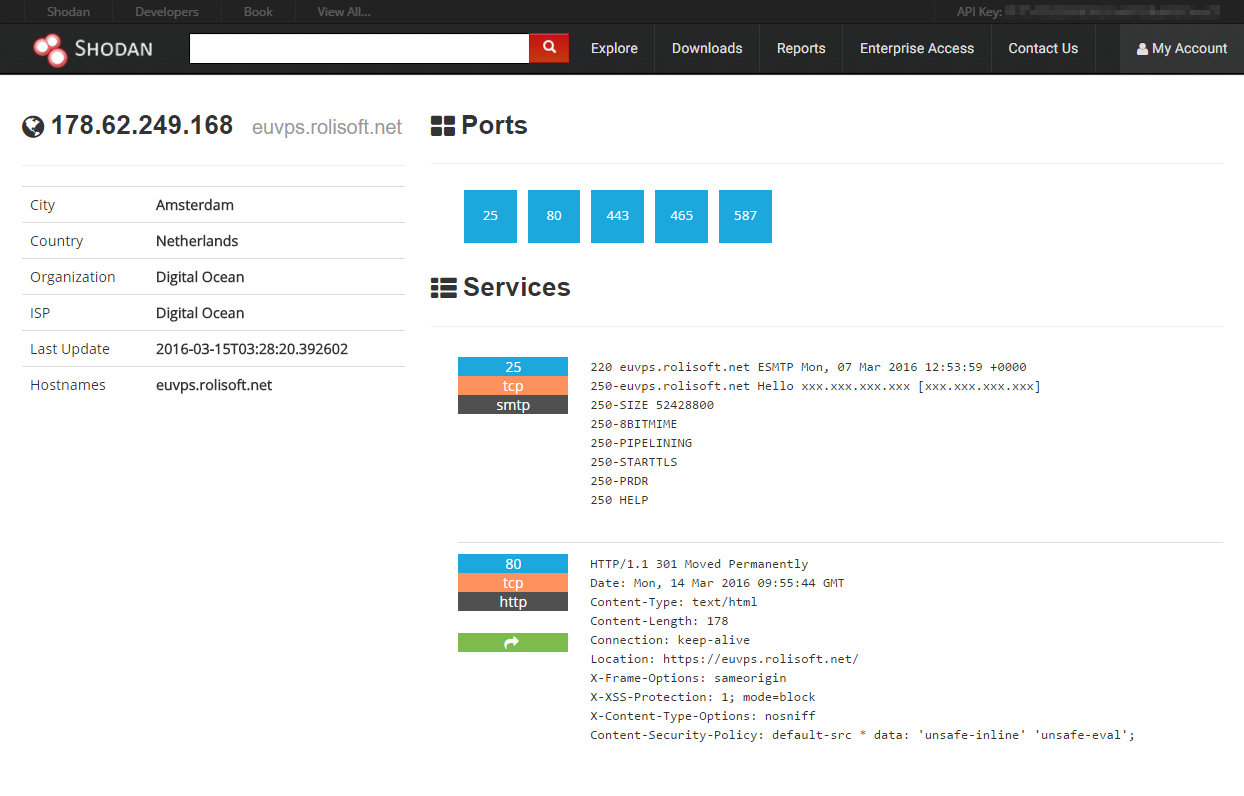
\includegraphics[scale=0.355]{shodan.png}
		\caption{Shodan report on an example IPv4 address}
		\label{shodanscr}
	\end{figure}
	
	In order to use Shodan data in the application developed within the scope of this thesis, the user has to create a free account at \url{https://shodan.io/} and specify the generated API key to the application via the \mintinline{bash}{--shodan-key} argument.
	
	Implementation-wise, the \mintinline{cpp}{ShodanScanner} component takes care of contacting the Shodan JSON API interface and retrieving the data available for the specified IP addresses. This component extends the \mintinline{cpp}{HostScanner} class, and as such it is possible to substitute the default scanner to Shodan data for any scanning needs.

\subsubsection{Censys} \label{censys}
\subsubsectionhu{Censys} \subsubsectionro{Censys}

	Censys\cite{censys15} is a project created and run by the Regents of the University of Michigan. Similarly to the previously discussed service, it also gathers its data by regular Internet-wide scanning efforts. It allows developers and security researchers to initiate structured queries, full-text search queries or raw SQL queries from their web interface or the exposed RESTful API. Figure \ref{censysscr} shows the data readily available on the service for a queried IP address.
	
	\begin{figure}[!htbp]
		\centering
		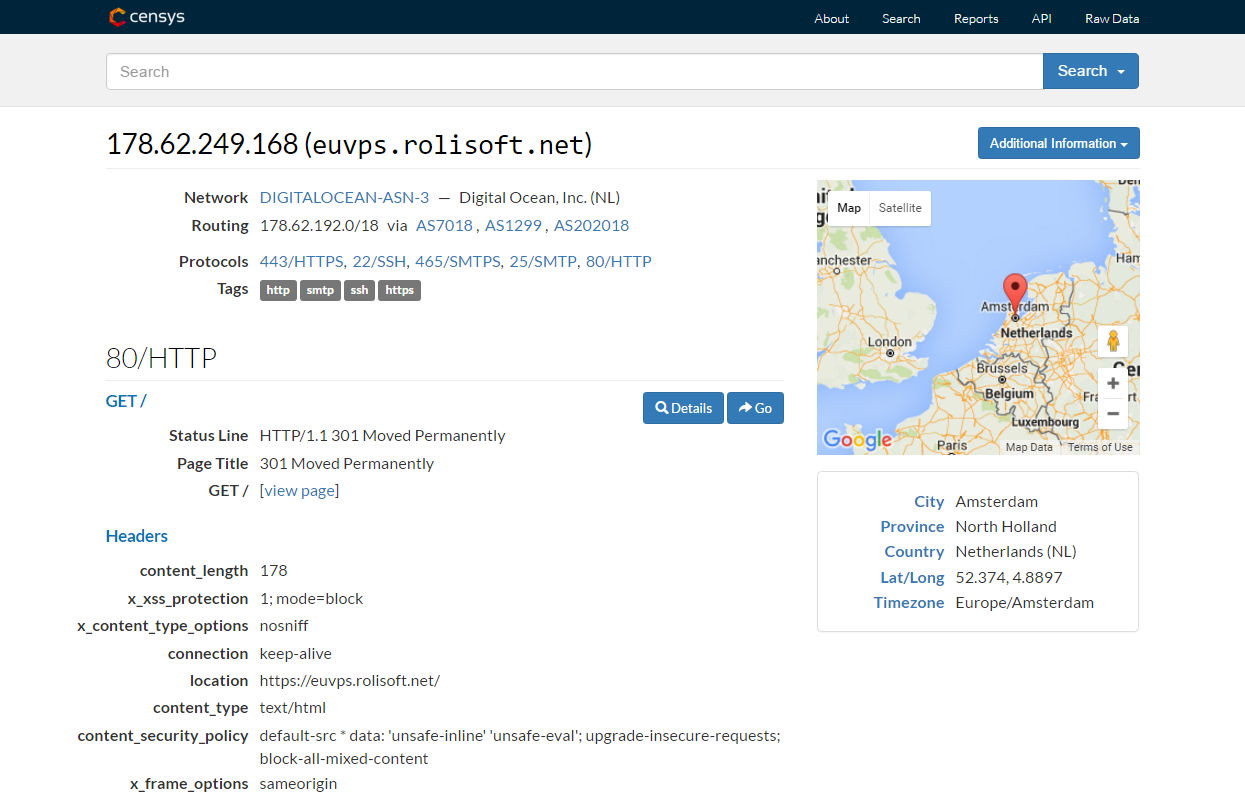
\includegraphics[scale=0.355]{censys.png}
		\caption{Censys report on an example IPv4 address}
		\label{censysscr}
	\end{figure}
	
	The network scanner in use by the service, namely ZMap\cite{zmap13}, and its various components are open-source. The raw data generated by this scanner during an Internet-wide scan is also available for download at the Censys website for anyone to freely consume.
	
	In order to use Censys data in the application developed within the scope of this thesis, the user has to create a free account at \url{https://censys.io/} and specify the generated UID and secret key to the application via the \mintinline{bash}{--censys-key} argument.
		
	Implementation-wise, the \mintinline{cpp}{CensysScanner} component takes care of contacting the Censys JSON API interface and retrieving the data available for the specified IP addresses. Similarly, this component also extends the \mintinline{cpp}{HostScanner} class, and as such it is possible to substitute the default scanner to Censys data for any scanning needs.
	
\subsubsection{Mr Looquer} \label{looquer}
\subsubsectionhu{Mr Looquer} \subsubsectionro{Mr Looquer}

	Mr Looquer\cite{looquer16} is a new open initiative with a focus on IPv6 intelligence, launched by two security researchers in the May of 2016.
	
	\begin{figure}[!htbp]
		\centering
		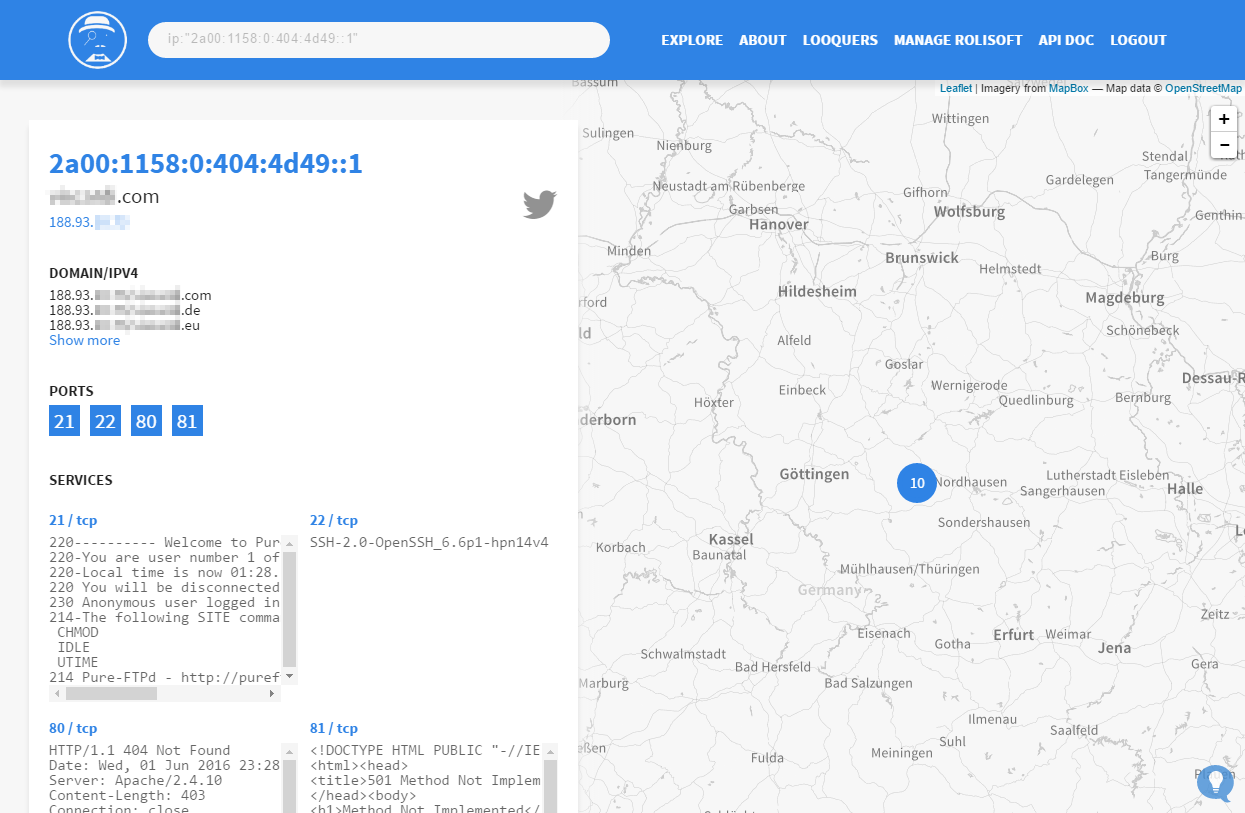
\includegraphics[scale=0.355]{looquer.png}
		\caption{Mr Looquer report on an example IPv6 address}
		\label{looquerscr}
	\end{figure}
	
	IPv6 has a much larger address space of $ 2^{128} $ addresses, as compared to the address space of IPv4 consisting of only $ 2^{32} $ addresses. Due to this increased address space, the technique used by the two aforementioned services (\textit{Shodan} and \textit{Censys}) of scanning the whole IPv4 address space, cannot be used in the case of IPv6. While the creators of \textit{ZMap} claim it is possible to scan the whole IPv4 address space under 5 minutes\cite{zmap13}, this speed would translate to $ 7.537 \cdot 10^{23} $ years for the IPv6 address space.
	
	As such, this service uses various data acquisition techniques to gather publicly used IPv6 addresses. One example would be the registered domain list various top-level domain NICs publish on request, such as Verisign's \textit{TLD Zone File Access Program}\cite{verisign16} for \textit{.com} and \textit{.net} TLDs. With this list, they can perform zone walking and use heuristics to infer relationships between the pointing domains and the reverse domains of both the IPv4 and IPv6 associated addresses.
	
	Similarly to the previously discussed services, it also allows developers and security researchers to initiate structured queries and full-text search queries from their web interface or the exposed RESTful API. Figure \ref{looquerscr} shows the data readily available on the service for a queried IP address.
	
	In order to use Mr Looquer data in the application developed within the scope of this thesis, the user has to create a free account at \url{https://mrlooquer.com/} and specify the generated API key to the application via the \mintinline{bash}{--looquer-key} argument.
		
	Implementation-wise, the \mintinline{cpp}{LooquerScanner} component takes care of contacting the Mr Looquer JSON API interface and retrieving the data available for the specified IP addresses. Similarly, this component also extends the \mintinline{cpp}{HostScanner} class, and as such it is possible to substitute the default scanner to Mr Looquer data for any scanning needs.

\subsubsection{Amalgamation}
\subsubsectionhu{Egyesítés} \subsubsectionro{Amalgamare}

	The \mintinline{cpp}{PassiveScanner} component of the application initiates the requested scan tasks on all three passive components, Shodan (s. \ref{shodan}), Censys (s. \ref{censys}) and Mr Looquer (s. \ref{looquer}), merging the results at the end.
	
	During the development phase of the application it was found that generally most services have had data on a requested IP address, but most of the times one of the services discovered more ports, have done much deeper analysis, or the information is more useful than at the competitor service.
	
	One concrete example would be where one service was somehow identified and banned from indexing an IP address, as shown in listing \ref{shodanban}, yet the other one was able to access it freely and has data available as a result, as shown in listing \ref{censysnoban}.
	
	\begin{listing}[H]
		\begin{minted}[style=pastie]{http}
			HTTP/1.1 403 You are banned from this site.  Please contact via a different client configuration if you believe that this is a mistake.
			Content-Type: text/html; charset=utf-8
			Date: Wed, 16 Mar 2016 01:17:18 GMT
			Retry-After: 5
			Server: Varnish
			X-Varnish: 2115087
			Content-Length: 590
			Connection: keep-alive
		\end{minted}
		\caption{Example response of 54.193.103.xyz for Shodan with a ban message}
		\label{shodanban}
	\end{listing}
		
	\begin{listing}[H]
		\begin{minted}[style=pastie]{http}
			HTTP/1.1 200 OK
			Content-Length: 3770
			Vary: Accept-Encoding
			Server: nginx/1.8.0
			Connection: keep-alive
			Last-Modified: Fri, 28 Aug 2015 19:43:39 GMT
			Content-Type: text/html
			Accept-Ranges: bytes
		\end{minted}
		\vspace{-5pt}
		\begin{minted}[style=borland,firstnumber=9]{html}
			 
			<!DOCTYPE html PUBLIC "-//W3C//DTD XHTML 1.1//EN" "http://www.w3.org/TR/xhtml11/DTD/xhtml11.dtd">
			<html xmlns="http://www.w3.org/1999/xhtml" xml:lang="en">
			<head>
			<!-- rest of the page omitted -->
		\end{minted}
		\caption{Example response of 54.193.103.xyz for Censys without a ban message}
		\label{censysnoban}
	\end{listing}

	It should also be noted that the underlying server software is not exposed to the banned party in listing \ref{shodanban}, but the non-banned party in listing \ref{censysnoban} has their request forwarded from the load-balancer to the backend, revealing itself to be ``nginx 1.8.0,'' a version with at least one \textbf{known remotely-exploitable vulnerability}\cite{nginxcve} at this time.

	In cases where both services return a service banner for a specific port, the longer banner is chosen during the amalgamation phase. One of the reasons for this decision was because ban messages are generally shorter\cite{qualys11} in order to avoid denial of service attacks. The other reason was that a longer banner generally means that the service in question possibly probed the port further (e.g. \mintinline{matlab}{STARTTLS} command sent to SMTP servers by Censys, but not by Shodan) which allows the pattern matching component described in \ref{patternmatch} to have more data available.

\subsection{External Reconnaissance} \label{nmapscan}
\subsectionhu{Külső Feltérképezés} \subsectionro{Scanare Externală}

	This section presents the \mintinline{cpp}{NmapScanner} component of the application which executes an external application in order to scan the requested ports, and then parses the results of the $3^{rd}$-party application for further processing within the $1^{st}$-party application.
	
	While the application implements a broad range of protocol scanners as discussed in sections \ref{icmpping} through \ref{udpscan}, with an unified interface for task parallelization as discussed in section \ref{tasks}, as a measure of redundancy, the users are given the choice of using an external scanner for their reconnaissance purposes.
	
	The component, as its name suggests, supports \textit{nmap} out-of-the-box as an alternative scanner, however, any $3^{rd}$-party application which generates nmap-compatible XML-based reports can be used. One such example is the \textit{masscan} scanner.
	
	In order to use nmap for scanning, the \mintinline{batch}{nmap} executable has to be accessible from within the \mintinline{batch}{PATH} environmental variable.

\newpage
\subsection{Class Hierarchy of Data Reconnaissance Components}
\subsectionhu{Adatszerző Komponensek Osztályhierarchiája} \subsectionro{Ierarhia de Clasă a Componentelor Colectoare de Date}

	\begingroup
	\hypersetup{linkcolor=blue}
	\begin{figure}[!htbp]
		\centering
		\begin{tikzpicture}[scale=0.85,transform shape]
			\node at (0,0) {HostScanner};
			\draw  (-1.5,0.5) rectangle (1.5,-0.5);
			\node at (-2,-3) {InternalScanner};
			\node at (-6,-3) {ArpPinger$^{\ref{arpping}}$};
			\node at (2,-3) {NmapScanner$^{\ref{nmapscan}}$};
			\draw  (-3.75,-2.5) rectangle (-0.25,-3.5);
			\draw  (0.25,-2.5) rectangle (3.75,-3.5);
			\draw  (-7.5,-2.5) rectangle (-4.5,-3.5);
			\node (v3) at (-6,-2.5) {};
			\node (v1) at (0,-0.5) {};
			\node (v2) at (-2,-2.5) {};
			\node (v4) at (2,-2.5) {};
			\draw [es] (v1) edge (v2);
			\draw [es] (v1) edge (v3);
			\draw [es] (v1) edge (v4);
			\node at (6,-3) {PassiveScanner};
			\draw  (4.5,-2.5) rectangle (7.5,-3.5);
			\node (v3_1) at (6,-2.5) {};
			\draw [es] (v1) edge (v3_1);
			\node at (3.5,-6) {ShodanScanner$^{\ref{shodan}}$};
			\draw  (1.5,-5.5) rectangle (5.5,-6.5);
			\node (v3_2) at (3.5,-5.5) {};
			\node at (8.5,-6) {CensysScanner$^{\ref{censys}}$};
			\draw  (6.5,-5.5) rectangle (10.5,-6.5);
			\node (v3_3) at (8.5,-5.5) {};
			\node (v5) at (6,-3.5) {};
			\draw [triangle 60-triangle 60] (v5) edge (v3_2);
			\draw [triangle 60-triangle 60] (v5) edge (v3_3);
			\node at (-2,-6) {ServiceScanner};
			\draw  (-3.75,-5.5) rectangle (-0.25,-6.5);
			\node at (-2,-9) {TcpScanner$^{\ref{tcpscan}}$};
			\node at (-6.25,-9) {IcmpScanner$^{\ref{icmpping}}$};
			\node at (2,-9) {UdpScanner$^{\ref{udpscan}}$};
			\draw  (-3.75,-8.5) rectangle (-0.25,-9.5);
			\draw  (0.25,-8.5) rectangle (3.75,-9.5);
			\draw  (-8,-8.5) rectangle (-4.5,-9.5);
			\node (v3_4) at (-6.25,-8.5) {};
			\node (v1_1) at (-2,-6.5) {};
			\node (v2_1) at (-2,-8.5) {};
			\node (v4_1) at (2,-8.5) {};
			\node (v6) at (-2,-3.5) {};
			\node (v7) at (-2,-5.5) {};
			\draw [dashed,-diamond]  (v6) edge (v7);
			\draw [es] (v1_1) edge (v2_1);
			\draw [es] (v1_1) edge (v3_4);
			\draw [es] (v1_1) edge (v4_1);
			\node at (6,-7.5) {LooquerScanner$^{\ref{looquer}}$};
			\draw  (4,-7) rectangle (8,-8);
			\node (v3_3_1) at (6,-7) {};
			\draw [triangle 60-triangle 60] (v5) edge (v3_3_1);
		\end{tikzpicture}
		\caption{Class Hierarchy of Data Reconnaissance Components}
		\label{classhierdata}
	\end{figure}
	\endgroup
	
\subsection{Multiplexing Task Runner} \label{tasks}
\subsectionhu{Feladatok Párhuzamosítása} \subsectionro{Paralelizarea Sarcinilor}
	
	A ``task'' in this context is defined to be the action of scanning a port on an IP address for a specified protocol. Such tasks mostly consist of sending IP packets back and forth followed by waiting for their acknowledgment or lack thereof.
	
	\begin{figure}[!htbp]
		\centering
		\begin{tikzpicture}
			\draw[color=gray,fill=gray] (0,-0.5) rectangle (-0.5,0);
			\draw[color=gray,fill=gray] (-1,-0.5) rectangle (-1.5,0);
			\draw[color=gray,fill=gray] (-2,-0.5) rectangle (-2.5,0);
			\draw[color=gray,fill=gray] (-3,-0.5) rectangle (-3.5,0);
			\draw[color=gray,fill=gray] (-4,-0.5) rectangle (-4.5,0);
			\draw (-5,0.25) -- (0.5,0.25);
			\draw (-5,-0.75) -- (0.5,-0.75);
			\node at (-2.25,0.75) {Queue of Tasks};
			\node (v1) at (0.5,-0.25) {};
			\draw [es](v1) -- (1.5,-0.25);
			\node at (-3.75,1.75) {Task Producer};
			\node at (-0.85,-2) {Enqueue due to I/O Wait};
			\node at (2.25,-0.25) {\huge \faCogs};
			\node at (2.25,-1.15) {Run Task};
			\node at (-5.6,1.75) {\huge \faPlusCircle};
			\node at (-3.75,-2) {\huge \faHourglassHalf};
			\node (v5) at (3,-0.25) {};
			\draw [es](v5) -- (4,0.75);
			\draw [es] plot[smooth, tension=.7] coordinates {(-4.5,-2) (-5.1,-1.55) (-5.3,-0.85) (-5.15,-0.35)};
			\draw [es] plot[smooth, tension=.7] coordinates {(-4.75,1.25) (-5.2,0.95) (-5.35,0.4) (-5.15,-0.15)};
			\node at (2,1.25) {\huge \faCheck};
			\node at (4.25,1.25) {Finished with Task};
			\draw [es] plot[smooth, tension=.7] coordinates {(3.15,-0.4) (3.55,-1.2) (3.1,-1.8) (1.75,-2)};
		\end{tikzpicture}
		\caption{Consumer-Producer Queue Process for Tasks}
		\label{taskqueue}
	\end{figure}
	
	As such, the parallelization method of using a thread pool and multiple threads is not efficient, since most threads would spend their time sleeping. Given the costly nature of thread spawning and managing, this is not efficient unless more lightweight threads can be spawned, such as `goroutines' in the Go programming language.
	
	The application instead implements a consumer-producer queue for storing and retrieving its tasks during scheduling, as shown in figure \ref{taskqueue}.
	
	\begin{figure}[!htbp]
		\centering
		\begin{tikzpicture}
			\node at (-4.5,1.5) {Send initial payload};
			\node at (0,1.5) {Check for reply};
			\node at (4,1.5) {Read reply};
			\node at (8.25,1.5) {Finish};
			\draw [es](-2.5,1.5) -- (-1.5,1.5);
			\draw [es](1.5,1.5) -- (2.75,1.5);
			\draw [es] plot[smooth, tension=.7] coordinates {(4,2) (3.25,2.5) (0.75,2.5) (0,2)};
			\draw [es](5.25,1.5) -- (7.25,1.5);
			\node at (2,3) {\textit{if no reply}};
			\node[align=center] at (6.25,2.25) {\textit{if wait expired}\\\textit{or got reply}};
			\node at (-4.5,0.25) {\textit{Phase 1}};
			\node at (1.75,0.25) {\textit{Phase 2}};
			\node at (8.25,0.25) {\textit{Phase 3}};
			\draw (-6,0.75) -- (-3,0.75);
			\draw (-1.25,0.75) -- (4.75,0.75);
			\draw (7.5,0.75) -- (9,0.75);
			\draw[color=gray] (-2.75,0.75) -- (-1.5,0.75);
			\draw[color=gray] (5,0.75) -- (7.25,0.75);
			\node[color=gray] at (-2.1,0.25) {I/O Wait};
			\node[color=gray] at (6.2,0.25) {I/O Wait};
		\end{tikzpicture}
		\caption{Phases of an UDP scan as implemented by component in section \ref{udpscan}}
		\label{taskudp}
	\end{figure}
	
	Figure \ref{taskudp} presents the phases of a UDP scan task. Each `phase' shows up in the queue as a different `task.' As a result of this scheduling and task multiplexing, one thread can handle all the scanning tasks needs.
	
	Figure \ref{seqtasks} represents the sequence diagram of the process through which tasks are initiated and placed onto the queue for multiplexed execution.
	
	\begin{figure}[!htbp]
		%	@startuml
		%	Application -> PortScannerFactory: IP:port list to be scanned
		%	PortScannerFactory --> Application: return tasks
		%	Application -> TaskRunner: list of tasks
		%	TaskRunner --> Application: results of tasks
		%	@enduml
		\centering
		\begin{tikzpicture}[yscale=-1]
			\draw[dash pattern=on 5.0pt off 5.0pt] (51pt,39.6094pt) -- (51pt,181.0156pt);
			\draw[dash pattern=on 5.0pt off 5.0pt] (220pt,39.6094pt) -- (220pt,181.0156pt);
			\draw[dash pattern=on 5.0pt off 5.0pt] (351pt,39.6094pt) -- (351pt,181.0156pt);
			\draw (8pt,3pt) rectangle (91pt,34.6094pt);
			\node at (15pt,10pt)[below right]{Application};
			\draw (8pt,180.0156pt) rectangle (91pt,211.625pt);
			\node at (15pt,187.0156pt)[below right]{Application};
			\draw (148pt,3pt) rectangle (289pt,34.6094pt);
			\node at (155pt,10pt)[below right]{PortScannerFactory};
			\draw (148pt,180.0156pt) rectangle (289pt,211.625pt);
			\node at (155pt,187.0156pt)[below right]{PortScannerFactory};
			\draw (303pt,3pt) rectangle (395pt,34.6094pt);
			\node at (310pt,10pt)[below right]{TaskRunner};
			\draw (303pt,180.0156pt) rectangle (395pt,211.625pt);
			\node at (310pt,187.0156pt)[below right]{TaskRunner};
			\draw[fill=black] (208.5pt,67.6094pt) -- (218.5pt,71.6094pt) -- (208.5pt,75.6094pt) -- (212.5pt,71.6094pt) -- cycle;
			\draw (51.5pt,71.6094pt) -- (214.5pt,71.6094pt);
			\node at (58.5pt,53.6094pt)[below right]{IP:port list to be scanned};
			\draw[fill=black] (62.5pt,97.9609pt) -- (52.5pt,101.9609pt) -- (62.5pt,105.9609pt) -- (58.5pt,101.9609pt) -- cycle;
			\draw[dash pattern=on 2.0pt off 2.0pt] (56.5pt,101.9609pt) -- (219.5pt,101.9609pt);
			\node at (68.5pt,83.9609pt)[below right]{return tasks};
			\draw[fill=black] (339pt,128.3125pt) -- (349pt,132.3125pt) -- (339pt,136.3125pt) -- (343pt,132.3125pt) -- cycle;
			\draw (51.5pt,132.3125pt) -- (345pt,132.3125pt);
			\node at (58.5pt,114.3125pt)[below right]{list of tasks};
			\draw[fill=black] (62.5pt,158.6641pt) -- (52.5pt,162.6641pt) -- (62.5pt,166.6641pt) -- (58.5pt,162.6641pt) -- cycle;
			\draw[dash pattern=on 2.0pt off 2.0pt] (56.5pt,162.6641pt) -- (350pt,162.6641pt);
			\node at (68.5pt,144.6641pt)[below right]{results of tasks};
		\end{tikzpicture}
		\caption{Sequence Diagram for Task Instantiation and Multiplexed Execution}
		\label{seqtasks}
	\end{figure}
	
	All tasks are implemented to use their sockets in a non-blocking mode, as such, as soon as one task has sent an IP packet and is about to wait for the results of its I/O operation, it instead goes into the back of the queue.
	
	Once the whole queue has been looped to collect the results of the previously initiated I/O operations, the aforementioned task will have a chance to collect its own operation results.
	
	The multiplexing task runner uses a lock-free thread-safe underlying queue container, namely the concurrent FIFO implementation in Boost, \mintinline{cpp}{boost::lock free::queue<T>}. As a result, for heavy workloads when excessive resources are available, the task runner can theoretically use multiple consumers on the same queue.
	
\subsection{Protocol Tokenization} \label{tokenizer}
\subsectionhu{Protokoll Értelmezés} \subsectionro{Interpretor de Protocoale}
	
	In order to improve the quality of the input for the CPE matcher component (further discussed in \ref{matchcpe}) and thereby minimizing the chances of false positives, the application makes a best effort to try recognizing and tokenizing the extracted service banners.
	
	The server replies are not fully parsed using a protocol-aware parser, instead it aims to either \textit{a)} extract server names, versions and operating system tags, or if that is not possible, \textit{b)} clean any known protocol strings, leaving only implementation-specific strings in the service banner.
	
	Currently, there are two protocol tokenizers implemented, and these are run in order of protocol popularity when a service banner needs to be cleaned. An API is exposed which does this, \mintinline{cpp}{ProtocolTokenizer::AutoTokenize(const std::string& banner)}.
	
	Figure \ref{seqtokenize} represents the sequence diagram of the process through which an unidentified service banner is automatically tokenized via the aforementioned exposed API.
	
	\begin{figure}[!htbp]
		%	@startuml
		%	ProtocolTokenizer -> HttpTokenizer: HTTP service banner
		%	HttpTokenizer --> ProtocolTokenizer: return tokens
		%	ProtocolTokenizer -> ThreeDigitTokenizer: service banner
		%	ThreeDigitTokenizer --> ProtocolTokenizer: return tokens
		%	@enduml
		\centering
		\begin{tikzpicture}[yscale=-1,scale=0.95,every node/.style={scale=0.95}]
			\draw[dash pattern=on 5.0pt off 5.0pt] (74pt,39.6094pt) -- (74pt,181.0156pt);
			\draw[dash pattern=on 5.0pt off 5.0pt] (216.5pt,39.6094pt) -- (216.5pt,181.0156pt);
			\draw[dash pattern=on 5.0pt off 5.0pt] (352.5pt,39.6094pt) -- (352.5pt,181.0156pt);
			\draw (8pt,3pt) rectangle (136pt,34.6094pt);
			\node at (15pt,10pt)[below right]{ProtocolTokenizer};
			\draw (8pt,180.0156pt) rectangle (136pt,211.625pt);
			\node at (15pt,187.0156pt)[below right]{ProtocolTokenizer};
			\draw (164.5pt,3pt) rectangle (265.5pt,34.6094pt);
			\node at (171.5pt,10pt)[below right]{HttpTokenizer};
			\draw (164.5pt,180.0156pt) rectangle (265.5pt,211.625pt);
			\node at (171.5pt,187.0156pt)[below right]{HttpTokenizer};
			\draw (279.5pt,3pt) rectangle (421.5pt,34.6094pt);
			\node at (286.5pt,10pt)[below right]{ThreeDigitTokenizer};
			\draw (279.5pt,180.0156pt) rectangle (421.5pt,211.625pt);
			\node at (286.5pt,187.0156pt)[below right]{ThreeDigitTokenizer};
			\draw[fill=black] (205pt,67.6094pt) -- (215pt,71.6094pt) -- (205pt,75.6094pt) -- (209pt,71.6094pt) -- cycle;
			\draw (74pt,71.6094pt) -- (211pt,71.6094pt);
			\node at (81pt,53.6094pt)[below right]{HTTP service banner};
			\draw[fill=black] (85pt,97.9609pt) -- (75pt,101.9609pt) -- (85pt,105.9609pt) -- (81pt,101.9609pt) -- cycle;
			\draw[dash pattern=on 2.0pt off 2.0pt] (79pt,101.9609pt) -- (216pt,101.9609pt);
			\node at (91pt,83.9609pt)[below right]{return tokens};
			\draw[fill=black] (340.5pt,128.3125pt) -- (350.5pt,132.3125pt) -- (340.5pt,136.3125pt) -- (344.5pt,132.3125pt) -- cycle;
			\draw (74pt,132.3125pt) -- (346.5pt,132.3125pt);
			\node at (81pt,114.3125pt)[below right]{service banner};
			\draw[fill=black] (85pt,158.6641pt) -- (75pt,162.6641pt) -- (85pt,166.6641pt) -- (81pt,162.6641pt) -- cycle;
			\draw[dash pattern=on 2.0pt off 2.0pt] (79pt,162.6641pt) -- (351.5pt,162.6641pt);
			\node at (91pt,144.6641pt)[below right]{return tokens};
		\end{tikzpicture}
		\caption{Sequence Diagram for Protocol-based Tokenization of Service Banners}
		\label{seqtokenize}
	\end{figure}
	
\subsubsection{Hyper-Text Transfer Protocol Tokenizer}
\subsubsectionhu{HTTP Értelmező} \subsubsectionro{Interpretor HTTP}
	
	The first tokenizer is \mintinline{cpp}{HttpTokenizer}, which decides whether the specified service banner contains a valid HTTP header and if so, proceeds to tokenize it. During tokenization, it will try to extract product names and version numbers from the appropriate places.
	
	The HTTP protocol has the `Server' and `X-Powered-By' header fields, which are generally used by software to indicate their name and version number. Unfortunately, the exact listing methodology is not standardized, as such different software may use different separators and notation to indicate their existence, version number, any vendor patches and possibly the operating system. Since these fields may have multiple products listed, the tokenizer makes sure to extract all the product names including any associated version numbers into separate tokens.
	
	\begin{listing}[H]
		\begin{minted}[style=pastie]{http}
			HTTP/1.1 200 OK
			Server: nginx/1.9.12 (Ubuntu)
			X-Powered-By: PHP/5.6.19
			Date: Fri, 11 Mar 2016 16:04:07 GMT
			Connection: close
		\end{minted}
		\caption{Example HTTP service banner}
		\label{httpsvcbnr}
	\end{listing}
	
	The HTTP service banner shown in listing \ref{httpsvcbnr} is produced by nginx 1.9.12 with PHP 5.6.19 installed on an Ubuntu distribution. When processed by the implemented tokenizer, it will produce the elements shown in listing \ref{httpsvcbnrtokens}.
	
	\begin{listing}[H]
		\begin{minted}[style=perldoc]{js}
			[
				// token,           later mapped to,           by component
				"nginx/1.9.12",  // cpe:/a:nginx:nginx:1.9.12, CpeDictionaryMatcher
				"Ubuntu",        // cpe:/o:canonical:ubuntu,   OperatingSystemIdentifier
				"PHP/5.6.19"     // cpe:/a:php:php:5.6.19,     CpeDictionaryMatcher
			]
		\end{minted}
		\caption{Extracted tokens from banner in listing \ref{httpsvcbnr}}
		\label{httpsvcbnrtokens}
	\end{listing}
	
	However, if the service banner being analyzed does not contain a valid HTTP header, the next tokenizer in order of protocol popularity to be tried is the \mintinline{cpp}{ThreeDigitTokenizer}, from now on referred to as the ``SMTP tokenizer'' for simplicity's sake.

\subsubsection{Generic Fallback Tokenizer}
\subsubsectionhu{Generikus Értelmező} \subsubsectionro{Interpretor Generic}
	
	The ``three-digit'' tokenizer is a general purpose solution for parsing protocols which use a three-digit response in their protocol to indicate message type/category of a given server reply. Such protocols include SMTP, NNTP, FTP and a few more. For these protocols, however, unfortunately, there is no standardized way to announce server name and version (like the `Server' header in the HTTP protocol) and as such the server name is generally casually announced in the informational level welcome message part of the service banner. The informational messages are generally within the range of $200-299$, however, this might vary depending on the actual protocol.
	
	\begin{listing}[H]
		\begin{minted}{matlab}
			220 example.com ESMTP Exim 4.87 #2 Fri, 11 Mar 2016 16:05:06 +0000
		\end{minted}
		\caption{Example SMTP service banner}
		\label{smtpsvcbnr}
	\end{listing}
		
	The SMTP service banner shown in listing \ref{smtpsvcbnr} is produced by Exim 4.87 listening on port 25. This banner is sent as a `greeting' as soon as the client connects to the server. This is favorable since no further protocol probes are required to be sent in order to get a processable service banner. When this banner is processed by the implemented tokenizer, it will produce the elements shown in listing \ref{smtpsvcbnrtokens}.
		
	\begin{listing}[H]
		\begin{minted}[style=perldoc]{js}
			[
				// token,                later mapped to,       by component
				"ESMTP Exim 4.87 #2", // cpe:/a:exim:exim:4.87, CpeDictionaryMatcher
			]
		\end{minted}
		\caption{Extracted tokens from banner in listing \ref{smtpsvcbnr}}
		\label{smtpsvcbnrtokens}
	\end{listing}
	
	It should be noted that the ``perfect'' token would be \mintinline{matlab}{Exim 4.87}, however as previously mentioned, the server name and version are not clearly advertised. As such, the processing of the banner starts by removing the protocol-specific strings, namely the response code (\mintinline{matlab}{220}), the host name (\mintinline{py}{example.com}), and the date (\mintinline{matlab}{Fri, 11 Mar 2016 16:05:06 +0000}). This leaves us with the implementation-specific string of \mintinline{matlab}{ESMTP Exim 4.87 #2}.
	
	The tokenizer implementation will try to remove as many non-implementation-specific tokens as possible, however in cases where a specific element cannot be determined with a high degree of certainty whether it is a protocol or implementation-specific string, the tokenizer will instead leave it in. This decision was made in order to ensure that the tokenizer does not remove any elements which are required for the CPE matcher during entry matching. If an element is left in falsely, it does not affect the scoring of the CPE matcher, however, if it was falsely removed, it could completely prevent the matching of that entry.
	
	If all of the implemented tokenizers fail to process a service banner, it will be sent to the next stage of discovery (usually to component described in \ref{matchcpe}) as one token, containing the whole service banner.
	
\subsection{Pattern Matching of Service Banners} \label{patternmatch}
\subsectionhu{Szerverek Minta-alapú Beazonosítása} \subsectionro{Identificare Software pe Bază de Model}

	The purpose of the \mintinline{cpp}{ServiceRegexMatcher} component of the application is to take the original full service banner (without any tokenization) as an input and match it against a database of regular expressions, which in turn are mapped to their own CPE names.

	\begin{listing}[H]
		\begin{minted}{matlab}
			^HTTP/1\.[01] \d{3}.*\r\nServer: nginx(?:/([\d.]+))?
		\end{minted}
		\caption{Example regular expression to match \mintinline{matlab}{cpe:/a:nginx:nginx}}
		\label{nginxregex}
	\end{listing}
	
	The example regular expression in listing \ref{nginxregex} matches against the response headers produced by the HTTP server software ``nginx''. See the service banner in listing \ref{httpsvcbnr} for an example that would be matched. Furthermore, the listed regular expression contains an optional capture group, which captures the version number. If the version number is listed in the service banner, the matcher component will return the CPE name \mintinline{matlab}{cpe:/a:nginx:nginx:1.9.12}, while without a version number listed, it will still return the CPE name \mintinline{matlab}{cpe:/a:nginx:nginx}.
	
	This behavior is different from the matcher described in section \ref{matchcpe}: whereas here a CPE name can be produced with high confidence with or without a known version number, the CPE dictionary-based matcher \textit{requires} a known version number, since it plays a pivotal role in the identifying and scoring process.
	
	Figure \ref{seqregex} represents the sequence diagram for the process of pattern-matching unidentified service banners. The ``BannerProcessor'' component of the sequence diagram acts as an intermediary, making sure to properly merge the returned information from the ``ServiceRegexMatcher'' component into the host object, as the latter class only contains the regular expression matching implementation.
		
	\begin{figure}[!htbp]
		%	@startuml
		%	Application -> BannerProcessor: service banners
		%	BannerProcessor -> ServiceRegexMatcher: match regexes
		%	ServiceRegexMatcher --> BannerProcessor: return CPE
		%	BannerProcessor --> Application: return CPE
		%	@enduml
		\centering
		\begin{tikzpicture}[yscale=-1]
			\draw[dash pattern=on 5.0pt off 5.0pt] (51pt,39.6094pt) -- (51pt,181.0156pt);
			\draw[dash pattern=on 5.0pt off 5.0pt] (169pt,39.6094pt) -- (169pt,181.0156pt);
			\draw[dash pattern=on 5.0pt off 5.0pt] (321pt,39.6094pt) -- (321pt,181.0156pt);
			\draw (8pt,3pt) rectangle (91pt,34.6094pt);
			\node at (15pt,10pt)[below right]{Application};
			\draw (8pt,180.0156pt) rectangle (91pt,211.625pt);
			\node at (15pt,187.0156pt)[below right]{Application};
			\draw (105pt,3pt) rectangle (229pt,34.6094pt);
			\node at (112pt,10pt)[below right]{BannerProcessor};
			\draw (105pt,180.0156pt) rectangle (229pt,211.625pt);
			\node at (112pt,187.0156pt)[below right]{BannerProcessor};
			\draw (243pt,3pt) rectangle (395pt,34.6094pt);
			\node at (250pt,10pt)[below right]{ServiceRegexMatcher};
			\draw (243pt,180.0156pt) rectangle (395pt,211.625pt);
			\node at (250pt,187.0156pt)[below right]{ServiceRegexMatcher};
			\draw[fill=black] (157pt,67.6094pt) -- (167pt,71.6094pt) -- (157pt,75.6094pt) -- (161pt,71.6094pt) -- cycle;
			\draw (51.5pt,71.6094pt) -- (163pt,71.6094pt);
			\node at (58.5pt,53.6094pt)[below right]{service banners};
			\draw[fill=black] (309pt,97.9609pt) -- (319pt,101.9609pt) -- (309pt,105.9609pt) -- (313pt,101.9609pt) -- cycle;
			\draw (169pt,101.9609pt) -- (315pt,101.9609pt);
			\node at (176pt,83.9609pt)[below right]{match regexes};
			\draw[fill=black] (180pt,128.3125pt) -- (170pt,132.3125pt) -- (180pt,136.3125pt) -- (176pt,132.3125pt) -- cycle;
			\draw[dash pattern=on 2.0pt off 2.0pt] (174pt,132.3125pt) -- (320pt,132.3125pt);
			\node at (186pt,114.3125pt)[below right]{return CPE};
			\draw[fill=black] (62.5pt,158.6641pt) -- (52.5pt,162.6641pt) -- (62.5pt,166.6641pt) -- (58.5pt,162.6641pt) -- cycle;
			\draw[dash pattern=on 2.0pt off 2.0pt] (56.5pt,162.6641pt) -- (168pt,162.6641pt);
			\node at (68.5pt,144.6641pt)[below right]{return CPE};
		\end{tikzpicture}
		\caption{Sequence Diagram for Pattern-based Matching of Service Banners}
		\label{seqregex}
	\end{figure}
	
\subsubsection{Inferring Products Without Express Announcement}
\subsubsectionhu{Identitás Kikövetkeztetése Névhírdetés Nélkül} \subsubsectionro{Deducerea Identității fără Anunțul cu Nume}
	
	While the example presented in listing \ref{nginxregex} is rather straight-forward, the pattern matcher method can be used in a more subtle way, for example, to match software which are not advertising their name or version number.
	
	\begin{listing}[H]
		\begin{minted}{matlab}
			^554 SMTP synchronization error\r\n
		\end{minted}
		\caption{Example regular expression to match \mintinline{matlab}{cpe:/a:exim:exim}}
		\label{eximregex}
	\end{listing}
	
	The example presented in listing \ref{eximregex} is a regular expression which matches an error message produced by the SMTP server software ``exim''. The reason why it is possible to determine this fact with high confidence is that exim is the only software returning this exact error message verbatim. Other SMTP servers will have a similar error message for this problem, with the same error code, but not with this same exact error message, as the messages themselves are not standardized byte-by-byte.
	
	\begin{multicols}{2}
		\begin{listing}[H]
			\begin{minted}{matlab}
				220 example-1.com ESMTP Sat, 12 Mar 2016 17:14:06 +0000
				EHLO client-1.com
				250-example-1.com Hello client-1.com [2a02:2f07:d18d:1100::cake]
				250-SIZE 52428800
				250-8BITMIME
				250-PIPELINING
				250-STARTTLS
				250-PRDR
				250 HELP
			\end{minted}
			\caption{Exim $\ge 4.83$}
			\label{eximwiprdr}
		\end{listing}
		\begin{listing}[H]
			\begin{minted}{matlab}
				220 example-2.com ESMTP Sat, 12 Mar 2016 16:12:25 +0000
				EHLO client-2.com
				250-example-2.com Hello client-2.com [2a02:2f07:d18d:1100::cake]
				250-SIZE 20971520
				250-8BITMIME
				250-PIPELINING
				250-AUTH PLAIN LOGIN
				250-STARTTLS
				250 HELP
			\end{minted}
			\caption{Exim $< 4.83$}
			\label{eximwoprdr}
		\end{listing}
	\end{multicols}
	
	It is even possible to associate a version number to the software behind the port. For example, exim has implemented ``SMTP Service Extension for Per-Recipient Data Responses'' in version 4.83, and it advertises this capability as `PRDR' after the handshake, as seen in listing \ref{eximwiprdr} versus the handshake of an older version in listing \ref{eximwoprdr}.
	
	A regular expression can be written to inspect the advertised capability list, and make an educated guess stating that the version of the software is 4.83 or older. This can be further improved by creating a pattern which matches a change which only applies to versions 4.86 and older, at which point it can be deduced that the inspected service banner was produced by exim between the versions of $4.83-4.86$.
	
	For open-source software, it is possible to compare the source between different releases and check which publicly visible string changed, in order to write a pattern for detecting that range of versions. Building such a database of patterns, however, is beyond the scope of this project, and would be more suited for a community-sourced project.
	
\subsection{Matching of CPE Tokens in Service Banners} \label{matchcpe}
\subsectionhu{Szerverek CPE-alapú Beazonosítása} \subsectionro{Identificare Software pe Bază de CPE}

	As discussed in \ref{vulndbs}, the \textit{National Institute of Standards and Technology} runs a \textit{National Vulnerability Database}. The \mintinline{cpp}{CpeDictionaryMatcher} component presented within this section makes use of the publicly distributed, freely available and daily updated \textit{Common Platform Enumeration Dictionary}.
	
	The \textit{CPE} is a naming scheme for hardware, software and operating systems\cite{cpe22}. Its v2.2 format is \mintinline{matlab}{cpe:/type:vendor:product:version:update:edition:language} where the `type' component can be \mintinline{matlab}{h} for `hardware', \mintinline{matlab}{o} for `operating system' and \mintinline{matlab}{a} for `application', while the rest of the components are self-explanatory.
	
	For example, the CPE name for ``nginx 1.3.9'' is \mintinline{matlab}{cpe:/a:igor_sysoev:nginx:1.3.9}.
	
	The aforementioned \textit{CPE dictionary} is a list of CPE names aggregated and maintained by NIST which are known to be vulnerable, i.e. have associated entries in the \textit{CVE database}.
	
	In listing \ref{nginxcpe} an excerpt is shown, presenting an entry from the dictionary for the ``nginx 1.9.9'' software.
	
	\begin{listing}[H]
		\begin{minted}[style=borland]{xml}
			<cpe-item name="cpe:/a:nginx:nginx:1.9.9">
				<title xml:lang="en-US">Nginx 1.9.9</title>
				<references>
					<reference href="http://nginx.org/">Product</reference>
					<reference href="http://nginx.org/en/CHANGES">Change Log</reference>
				</references>
				<cpe-23:cpe23-item name="cpe:2.3:a:nginx:nginx:1.9.9:*:*:*:*:*:*:*"/>
			</cpe-item>
		\end{minted}
		\caption{CPE entry for nginx 1.9.9}
		\label{nginxcpe}
	\end{listing}
	
	Unfortunately, the CPE names are not advertised in the service banners, nor is there a direct standard to map CPE names to service banners, or any other straight-forward solution on mapping them. In paper \cite{shovat15}, the authors have tackled the same issue of processing and mapping the entries to service banners. The method presented within the paper was the basis for the implementation of the CPE matcher component in the application developed within the scope of this thesis.
	
\subsubsection{Implementation Overview}
\subsubsectionhu{Kivitelezés Áttekintése} \subsubsectionro{Prezentare Generală}
	
	The current implementation of the CPE matcher component loads a preprocessed version of the CPE dictionary into its memory, where the CPE names are tokenized, and irrelevant data (such as product links) are stripped for memory efficiency. Listing \ref{ciscotokens} presents the tokens loaded into memory for an example CPE name. For the exact implementation, see the structures within the header file of the \mintinline{cpp}{CpeDictionaryMatcher} class.
	
	\begin{listing}[H]
		\begin{minted}[style=perldoc]{js}
			CpeEntry {
				// cpe:/o:cisco:ios
				"ProductSpecificTokens": ["cisco", "ios"],
				"Versions": [
					CpeVersionEntry {
						// cpe:/o:cisco:ios:12.2sxi
						"VersionNumber": "12.2",
						"VersionSpecificTokens": ["sxi"]
					},
					CpeVersionEntry {
						// cpe:/o:cisco:ios:12.2sxh
						"VersionNumber": "12.2",
						"VersionSpecificTokens": ["sxh"]
					}
					// [further versions omitted]
				]
			}
		\end{minted}
		\caption{Approximate internal representation of tokens for \mintinline{matlab}{cpe:/o:cisco:ios:12.2sxi}}
		\label{ciscotokens}
	\end{listing}
	
	During the tokenization process, the `vendor' and `product' components of the CPE name are matched against the regular expression \mintinline{matlab}{([a-z][a-z0-9]+)} in order to extract all words individually, ignoring one character words and those starting with a number.
	
	Doing so, the resulting array will end up looking like \mintinline[style=vs]{js}{["apache", "tomcat"]} for the example CPE name \mintinline{matlab}{cpe:/a:apache:tomcat:4.1.36}.
	
	The version component of the CPE contains in some cases irrelevant characters or non-standard version notation. In order to work around this, the version number is extracted from the component using the regular expression \mintinline{matlab}{\d+\.(?:\d+\.)*\d+}, which requires at least two numbers separated by a dot.
	
	If the version number contains any words, these are extracted with the aforementioned regular expression in the tokenization phase. As such, in the case of the CPE name \mintinline{matlab}{cpe:/o:cisco:ios:12.2sxi}, there will be an array of `version-specific tokens' consisting of the word \mintinline[style=vs]{js}{["sxi"]}.
	
	During CPE matching, the entries are iterated, checking to see if the product-specific tokens match. If all of the tokens match, the entry-specific versions are iterated, checking to see if any of the version numbers are present in the input. If so, version-specific tokens are checked as well. A version is not considered a match if the version number matches, but even just one of the version-specific tokens do not.
	
	There are entries where multiple versions may match within the same product, such edge cases are discussed in subsection \ref{cpeedges}. In situations like these, a single version number is selected as the winner, which is determined by the distance of the tokens to the version number. The further a token is from the version number, the lesser it is considered to be relevant.
	
	For product names, however, if multiple products (including their complete version numbers with tokens) match, all of the matches will be returned. The reason for this decision is because a service banner may name multiple software in use, but not multiple versions of the same software to be in use. In listing \ref{httpsvcbnr}, the service banner reveals the existence of three products, namely ``nginx 1.9.12,'' ``PHP 5.6.19'' and ``Ubuntu.''
	
	Figure \ref{seqtoken} represents the sequence diagram of the process through which an unidentified service banner is tokenized and matched against the database of known tokens. The ``ProtocolTokenizer'' component of the sequence diagram has its own sequence diagram visible in figure \ref{seqtokenize}. The ``BannerProcessor'' component acts as an intermediary, making sure to properly merge the returned information from the ``CpeDictionaryMatcher'' component into the host object, as the latter class only contains the token matching implementation.
	
	\begin{figure}[!htbp]
		%	@startuml
		%	Application -> BannerProcessor: service banners
		%	BannerProcessor -> ProtocolTokenizer: service banner
		%	ProtocolTokenizer -> BannerProcessor: return tokens
		%	BannerProcessor -> CpeDictionaryMatcher: extracted tokens
		%	CpeDictionaryMatcher --> BannerProcessor: return CPE
		%	BannerProcessor --> Application: return CPE
		%	@enduml
		\centering
		\begin{tikzpicture}[yscale=-1,scale=0.8,every node/.style={scale=0.8}]
			\draw[dash pattern=on 5.0pt off 5.0pt] (51pt,39.6094pt) -- (51pt,241.7188pt);
			\draw[dash pattern=on 5.0pt off 5.0pt] (169pt,39.6094pt) -- (169pt,241.7188pt);
			\draw[dash pattern=on 5.0pt off 5.0pt] (309pt,39.6094pt) -- (309pt,241.7188pt);
			\draw[dash pattern=on 5.0pt off 5.0pt] (464pt,39.6094pt) -- (464pt,241.7188pt);
			\draw (8pt,3pt) rectangle (91pt,34.6094pt);
			\node at (15pt,10pt)[below right]{Application};
			\draw (8pt,240.7188pt) rectangle (91pt,272.3281pt);
			\node at (15pt,247.7188pt)[below right]{Application};
			\draw (105pt,3pt) rectangle (229pt,34.6094pt);
			\node at (112pt,10pt)[below right]{BannerProcessor};
			\draw (105pt,240.7188pt) rectangle (229pt,272.3281pt);
			\node at (112pt,247.7188pt)[below right]{BannerProcessor};
			\draw (243pt,3pt) rectangle (371pt,34.6094pt);
			\node at (250pt,10pt)[below right]{ProtocolTokenizer};
			\draw (243pt,240.7188pt) rectangle (371pt,272.3281pt);
			\node at (250pt,247.7188pt)[below right]{ProtocolTokenizer};
			\draw (385pt,3pt) rectangle (539pt,34.6094pt);
			\node at (392pt,10pt)[below right]{CpeDictionaryMatcher};
			\draw (385pt,240.7188pt) rectangle (539pt,272.3281pt);
			\node at (392pt,247.7188pt)[below right]{CpeDictionaryMatcher};
			\draw[fill=black] (157pt,67.6094pt) -- (167pt,71.6094pt) -- (157pt,75.6094pt) -- (161pt,71.6094pt) -- cycle;
			\draw (51.5pt,71.6094pt) -- (163pt,71.6094pt);
			\node at (58.5pt,53.6094pt)[below right]{service banners};
			\draw[fill=black] (297pt,97.9609pt) -- (307pt,101.9609pt) -- (297pt,105.9609pt) -- (301pt,101.9609pt) -- cycle;
			\draw (169pt,101.9609pt) -- (303pt,101.9609pt);
			\node at (176pt,83.9609pt)[below right]{service banner};
			\draw[fill=black] (180pt,128.3125pt) -- (170pt,132.3125pt) -- (180pt,136.3125pt) -- (176pt,132.3125pt) -- cycle;
			\draw (174pt,132.3125pt) -- (308pt,132.3125pt);
			\node at (186pt,114.3125pt)[below right]{return tokens};
			\draw[fill=black] (452pt,158.6641pt) -- (462pt,162.6641pt) -- (452pt,166.6641pt) -- (456pt,162.6641pt) -- cycle;
			\draw (169pt,162.6641pt) -- (458pt,162.6641pt);
			\node at (176pt,144.6641pt)[below right]{extracted tokens};
			\draw[fill=black] (180pt,189.0156pt) -- (170pt,193.0156pt) -- (180pt,197.0156pt) -- (176pt,193.0156pt) -- cycle;
			\draw[dash pattern=on 2.0pt off 2.0pt] (174pt,193.0156pt) -- (463pt,193.0156pt);
			\node at (186pt,175.0156pt)[below right]{return CPE};
			\draw[fill=black] (62.5pt,219.3672pt) -- (52.5pt,223.3672pt) -- (62.5pt,227.3672pt) -- (58.5pt,223.3672pt) -- cycle;
			\draw[dash pattern=on 2.0pt off 2.0pt] (56.5pt,223.3672pt) -- (168pt,223.3672pt);
			\node at (68.5pt,205.3672pt)[below right]{return CPE};
		\end{tikzpicture}
		\caption{Sequence Diagram for CPE Token-based Matching of Service Banners}
		\label{seqtoken}
	\end{figure}
	
\subsubsection{Handling of Edge Cases} \label{cpeedges}
\subsubsectionhu{Élesetek Kezelése} \subsubsectionro{Soluționarea Cazurilor de Margine}

	The now-defunct \textit{Sun Microsystems} vendor identifier is ``sun'', resulting in CPE names such as \mintinline{matlab}{cpe:/a:sun:jre}, \mintinline{matlab}{cpe:/a:sun:jdk} and \mintinline{matlab}{cpe:/o:sun:solaris:10.0}. The problematic part with this token is that most protocols, such as SMTP and HTTP, return the current date in the RFC 1123 format\cite{rfc2616}, which looks like this: ``Sun, 14 Mar 2016 16:33:02 GMT''.
	
	The first component of the date is the shortened three-letter English name of the day, which on Sundays is ``Sun''. This introduces a `random' element into the equation, as the scoring system of the CPE matcher would rank CPEs from the \textit{Sun Microsystems} vendor higher, as the ``sun'' token is now present in the service banner.
	
	\begin{listing}[H]
		\begin{minted}{matlab}
			Cisco IOS Software, s72033_rp Software (s72033_rp-IPSERVICESK9_WAN-M), Version 12.2(33)SXI3, RELEASE SOFTWARE (fc2)
			Technical Support: http://www.cisco.com/techsupport
			Copyright (c) 1986-2009 by Cisco Systems, Inc.
			Compiled Tue 27-Oct-09 11:12 by prod_
		\end{minted}
		\caption{Example telnet service banner of Cisco routers}
		\label{ciscosvcbnr}
	\end{listing}

	Another example would be Cisco's version numbering and their telnet service banners. In listing \ref{ciscosvcbnr}, the service banner of \mintinline{matlab}{cpe:/o:cisco:ios:12.2sxi3} is shown. The problematic part arises from the fact that Cisco has the same version number $12.2$ with the patch level specified as ``by'': \mintinline{matlab}{cpe:/o:cisco:ios:12.2by}.
	
	If one were to tokenize the two CPE names, they would get two arrays which would look like these: \mintinline[style=vs]{js}{["cisco", "ios", "sxi"]} and \mintinline[style=vs]{js}{["cisco", "ios", "by"]}. The version number and the first two tokens from both arrays would match, however so would both ``sxi'' and ``by''. On lines 3 and 4 of \ref{ciscosvcbnr} the copyright and compilation notices both contain the word/token ``by''.

	The aforementioned ShoVAT\cite{shovat15} paper solved this issue by weighing tokens around the version number more than those further from the version number, which solution is ultimately what the application written within the scope of this thesis has also settled with on one hand.
	
	However, a different solution was also implemented to combat this. The protocol tokenizer component discussed in \ref{tokenizer} was developed for the express purpose of extracting product names and versions from a service banner, or if that is not possible, then removing irrelevant parts, such as dates and non-informational messages.
	
\subsection{Identification of Operating Systems} \label{opsysmatcher}
\subsectionhu{Operációs Rendszerek Beazonosítása} \subsectionro{Identificarea Sistemelor de Operare}

	The techniques discussed in the sections \ref{patternmatch} and \ref{matchcpe} cannot be used to identify the operating system of the scanned host, as in most of the cases, these services do not advertise the underlying operating system the server software is running on.
	
	The application implemented within the scope of this thesis supports the identification of \textbf{Debian}, \textbf{Ubuntu}, \textbf{Red Hat}, \textbf{CentOS} and \textbf{Fedora} Linux distributions. For these distributions, the exact version number of the installed operating system can be deduced as well, not just the name.
	
	After successful identification, the CPE names and CVE vulnerabilities discovered on the system can be traced back to a specific package in the distribution's package manager, thus allowing \textit{vulnerability validation} (further discussed in \ref{vulnvalid}) by checking with the vendor, whether the discovered vulnerability actually affects the active installation or not.
	
	Support for \textbf{Windows} is currently limited: the operating system itself can be identified, however due to the lack of a centralized package manager, the CPE to package name and vulnerability validation functions are not available for scanned hosts running such operating systems.
	
	Identification of the operating systems based on the gathered results are done by separate \mintinline{cpp}{*Identifier} classes, where one implementation exists for each operating system, and they are invoked in order of popularity until a certain hit is produced.
	
	A common theme within these identifier implementations is analyzing the discovered SSH server, as the SSH protocol requires every server to identify themselves accurately for compatibility reasons.
	
	While most server software have an option to decrease the verbosity of the announced software information (such as name, version, patch level and operating system) due to the aforementioned protocol requirements, no SSH server (at least on the supported Linux distributions) allows silencing the information contained within the service banner of the SSH service.
	
	In Debian or Debian-based (such as Ubuntu) distributions, the \mintinline{matlab}{openssh} package is modified to further increase the amount of information announced, as its service banner also contains the installed security patch version number as well. This behavior can be turned off using the \mintinline{matlab}{DebianBanner} configuration option, however, it is on by default, and it is not common practice to turn it off after a fresh installation.
	
	If the extended version information announcement is not turned off, the distribution can be deduced from that, otherwise, the SSH server version number can be looked up against the list of bundled OpenSSH packages in each distribution generation, as shown in table \ref{debsshvers} for Debian or table \ref{ubnsshvers} for Ubuntu.
	
	The ``Enterprise Linux'' distributions do not suffer from this, however, due to the nature of the release lifecycle of these distributions, multiple years may pass between the versions, and as such the SSH server version number will increase in the newer versions, but stay the same in the current generation ones.
	
	As a result, if the software is otherwise certain that the host is actually running one of these distributions, it is possible to tell the exact version number of a host running Red Hat or CentOS, by matching the version number of the discovered SSH service to the list of the version numbers of the SSH packages as shipped between different versions of the specific operating system distribution, as shown in table \ref{elsshvers}.
	
	\begin{table}[H]
		\centering
		\begin{tabular}{|rl|}
			\hline
			\textbf{Debian} & \textbf{OpenSSH} \\ \hline
			Stretch (9) & 7.2p2 \\
			Jessie (8) & 6.7p1 \\
			Wheezy (7) & 6.6p1 -- 6.0p1 \\
			Squeeze (6) & 5.5p1 \\
			Lenny (5) & 5.1p1 \\
			Etch (4) & 4.3p2 \\
			Sarge (3.1) & 3.8.1p1 \\
			Woody (3) & 3.4p1 \\ \hline
		\end{tabular}
		\caption{Bundled OpenSSH packages in each Debian distribution}
		\label{debsshvers}
	\end{table}
		
	\begin{table}[H]
		\centering
		\begin{tabular}{|rl|}
			\hline
			\textbf{Ubuntu} & \textbf{OpenSSH} \\ \hline
			Xenial (16.04) & 7.2p2 \\
			Wily (15.10) & 6.9p1 \\
			Vivid (15.04) & 6.7p1 \\
			Utpic (14.10) & 6.6p1 \\
			Trusty (14.04.4) & 6.6.1p1 \\
			Trusty (14.04) & 5.9p1 \\
			Lucid (10.04) & 5.3p1 \\
			Hardy (8.04) & 4.7p1 \\
			Dapper (6.06) & 4.2p1 \\ \hline
		\end{tabular}
		\caption{Bundled OpenSSH packages in each Ubuntu distribution}
		\label{ubnsshvers}
	\end{table}
			
	\begin{table}[H]
		\centering
		\begin{tabular}{|rl|}
			\hline
			\textbf{E.L.} & \textbf{OpenSSH} \\ \hline
			7 & 6.6.1p1 \\
			6 & 6.6p1, 5.3, 5.2p1 \\
			5 & 4.3 \\
			4 & 3.9 \\ \hline
		\end{tabular}
		\caption{Bundled OpenSSH packages in each Red Hat/CentOS distribution}
		\label{elsshvers}
	\end{table}
	
	Tables \ref{debsshvers}, \ref{ubnsshvers} and \ref{elsshvers} were compiled manually, by navigating to the web interface of each distribution's package manager, and looking up historical release information for the ``openssh'' package. This list is hard-coded into the application, as it is not bound to change anymore.
	
	For operating systems where only identification is supported, without further interactions, such as Windows, the identification is achieved by analyzing the discovered service banners for various tokens unique to the platform. For example, the Windows identifier will look for ``Cygwin'' or ``Win32'' in the SSH banner, or the existence of platform-exclusive server software, such as an HTTP server identify itself as ``Microsoft IIS''.
	
	Figure \ref{seqos} represents the sequence diagram for the process through which a collection of service banners are processed on a per-host basis, in order to determine the operating system and version of the host. The ``*Identifier'' component of the sequence diagram represents all the implemented operating system identifier classes, which are enumerated in order of popularity until an implementation successfully returns.
	
	\begin{figure}[!htbp]
		%	@startuml
		%	Application -> OperatingSystemIdentifier: service banners of host
		%	OperatingSystemIdentifier -> _Identifier: service banners of host
		%	_Identifier --> OperatingSystemIdentifier: return OS CPE
		%	OperatingSystemIdentifier --> Application: return OS CPE
		%	@enduml
		\centering
		\begin{tikzpicture}[yscale=-1]
			\draw[dash pattern=on 5.0pt off 5.0pt] (51pt,39.6094pt) -- (51pt,181.0156pt);
			\draw[dash pattern=on 5.0pt off 5.0pt] (208pt,39.6094pt) -- (208pt,181.0156pt);
			\draw[dash pattern=on 5.0pt off 5.0pt] (365.5pt,39.6094pt) -- (365.5pt,181.0156pt);
			\draw (8pt,3pt) rectangle (91pt,34.6094pt);
			\node at (15pt,10pt)[below right]{Application};
			\draw (8pt,180.0156pt) rectangle (91pt,211.625pt);
			\node at (15pt,187.0156pt)[below right]{Application};
			\draw (118pt,3pt) rectangle (295pt,34.6094pt);
			\node at (125pt,10pt)[below right]{OperatingSystemIdentifier};
			\draw (118pt,180.0156pt) rectangle (295pt,211.625pt);
			\node at (125pt,187.0156pt)[below right]{OperatingSystemIdentifier};
			\draw (325.5pt,3pt) rectangle (401.5pt,34.6094pt);
			\node at (332.5pt,10pt)[below right]{*Identifier};
			\draw (325.5pt,180.0156pt) rectangle (401.5pt,211.625pt);
			\node at (332.5pt,187.0156pt)[below right]{*Identifier};
			\draw[fill=black] (196.5pt,67.6094pt) -- (206.5pt,71.6094pt) -- (196.5pt,75.6094pt) -- (200.5pt,71.6094pt) -- cycle;
			\draw (51.5pt,71.6094pt) -- (202.5pt,71.6094pt);
			\node at (58.5pt,53.6094pt)[below right]{service banners of host};
			\draw[fill=black] (353.5pt,97.9609pt) -- (363.5pt,101.9609pt) -- (353.5pt,105.9609pt) -- (357.5pt,101.9609pt) -- cycle;
			\draw (208.5pt,101.9609pt) -- (359.5pt,101.9609pt);
			\node at (215.5pt,83.9609pt)[below right]{service banners of host};
			\draw[fill=black] (219.5pt,128.3125pt) -- (209.5pt,132.3125pt) -- (219.5pt,136.3125pt) -- (215.5pt,132.3125pt) -- cycle;
			\draw[dash pattern=on 2.0pt off 2.0pt] (213.5pt,132.3125pt) -- (364.5pt,132.3125pt);
			\node at (225.5pt,114.3125pt)[below right]{return OS CPE};
			\draw[fill=black] (62.5pt,158.6641pt) -- (52.5pt,162.6641pt) -- (62.5pt,166.6641pt) -- (58.5pt,162.6641pt) -- cycle;
			\draw[dash pattern=on 2.0pt off 2.0pt] (56.5pt,162.6641pt) -- (207.5pt,162.6641pt);
			\node at (68.5pt,144.6641pt)[below right]{return OS CPE};
		\end{tikzpicture}
		\caption{Sequence Diagram for Operating System Identification}
		\label{seqos}
	\end{figure}
	
\subsection{Vulnerability Lookup}
\subsectionhu{Sebezhetőségek Lekérdezése} \subsectionro{Căutarea Vulnerabilităților}
	
	This section presents the methodology which allows the application to find the vulnerabilities of an identified CPE name.
	
	The vulnerability database in used by the application is \textit{NIST}'s \textit{National Vulnerability Database}, as discussed in section \ref{vulndbs}, which is an XML file containing \textit{CVE} entries. A CVE entry represents a single vulnerability, containing its description, \textit{CVSS} scoring (as discussed in \ref{cvss}), and a list of the affected CPE names (as briefly mentioned in \ref{matchcpe}).
	
	When searching for vulnerabilities, the application traverses the list of CVE entries, and checks if any of the CVE entries' \mintinline{xml}{<vulnerable-software-list />} contains the CPE name in question.
	
	When comparing CPE entries, all components of the CPE have to match in order to declare the application vulnerable. It should be noted, that fields which do not have a value are considered to be wildcard components, and match to any value.
	
	For example, \mintinline{matlab}{cpe:/o:microsoft:windows:10} refers to \textit{Windows 10}, while the \textit{Hungarian} version of Windows 10 is referred to as \mintinline{matlab}{cpe:/o:microsoft:windows:10:::hu}. When referred specifically, it means that the other language versions of the same product are not affected. However, if a CVE entry only refers to \mintinline{matlab}{cpe:/o:microsoft:windows:10}, it is assumed that other fields are set to \mintinline{matlab}{*}, being equal to \mintinline{matlab}{cpe:/o:microsoft:windows:10:*:*:*}, and therefore making the Hungarian version of the product affected as well.
	
	Figure \ref{seqnvd} presents the sequence diagram of the process through which CPE names are resolved to CVE entries within the application. The ``Database'' component of the diagram represents the aforementioned National Vulnerability Database, however, the application itself is not querying the published XML file directly, it instead is querying a SQLite database, which is filled with the relevant fields of the published XML file. This is done in order to increase performance and lower memory consumption of each lookup request.
	
	\begin{figure}[!htbp]
		%	@startuml
		%	Application -> VulnerabilityLookup: CPEs w/ version
		%	VulnerabilityLookup -> Database: find affected
		%	Database -> VulnerabilityLookup: raw CVE entries
		%	VulnerabilityLookup -> Application: return processed CVEs
		%	@enduml
		\centering
		\begin{tikzpicture}[yscale=-1]
			\draw[dash pattern=on 5.0pt off 5.0pt] (51pt,39.6094pt) -- (51pt,181.0156pt);
			\draw[dash pattern=on 5.0pt off 5.0pt] (210.5pt,39.6094pt) -- (210.5pt,181.0156pt);
			\draw[dash pattern=on 5.0pt off 5.0pt] (330.5pt,39.6094pt) -- (330.5pt,181.0156pt);
			\draw (8pt,3pt) rectangle (91pt,34.6094pt);
			\node at (15pt,10pt)[below right]{Application};
			\draw (8pt,180.0156pt) rectangle (91pt,211.625pt);
			\node at (15pt,187.0156pt)[below right]{Application};
			\draw (139.5pt,3pt) rectangle (277.5pt,34.6094pt);
			\node at (146.5pt,10pt)[below right]{VulnerabilityLookup};
			\draw (139.5pt,180.0156pt) rectangle (277.5pt,211.625pt);
			\node at (146.5pt,187.0156pt)[below right]{VulnerabilityLookup};
			\draw (291.5pt,3pt) rectangle (366.5pt,34.6094pt);
			\node at (298.5pt,10pt)[below right]{Database};
			\draw (291.5pt,180.0156pt) rectangle (366.5pt,211.625pt);
			\node at (298.5pt,187.0156pt)[below right]{Database};
			\draw[fill=black] (198.5pt,67.6094pt) -- (208.5pt,71.6094pt) -- (198.5pt,75.6094pt) -- (202.5pt,71.6094pt) -- cycle;
			\draw (51.5pt,71.6094pt) -- (204.5pt,71.6094pt);
			\node at (58.5pt,53.6094pt)[below right]{CPEs w/ version};
			\draw[fill=black] (319pt,97.9609pt) -- (329pt,101.9609pt) -- (319pt,105.9609pt) -- (323pt,101.9609pt) -- cycle;
			\draw (210.5pt,101.9609pt) -- (325pt,101.9609pt);
			\node at (217.5pt,83.9609pt)[below right]{find affected};
			\draw[fill=black] (221.5pt,128.3125pt) -- (211.5pt,132.3125pt) -- (221.5pt,136.3125pt) -- (217.5pt,132.3125pt) -- cycle;
			\draw (215.5pt,132.3125pt) -- (330pt,132.3125pt);
			\node at (227.5pt,114.3125pt)[below right]{raw CVE entries};
			\draw[fill=black] (62.5pt,158.6641pt) -- (52.5pt,162.6641pt) -- (62.5pt,166.6641pt) -- (58.5pt,162.6641pt) -- cycle;
			\draw (56.5pt,162.6641pt) -- (209.5pt,162.6641pt);
			\node at (68.5pt,144.6641pt)[below right]{return processed CVEs};
		\end{tikzpicture}
		\caption{Sequence Diagram for Vulnerability Lookup}
		\label{seqnvd}
	\end{figure}
	
	Section \ref{matchcpe} briefly introduces the CPE notation, giving an example to ``nginx 1.9.9'' in listing \ref{nginxcpe}. Continuing this example, listing \ref{nginxcve} presents the raw XML entry for the CVE item ``CVE-2016-0742'', which affects the aforementioned server software by having its CPE name in the list of vulnerable software.
	
	\begin{listing}[H]
		\begin{minted}[style=borland]{xml}
			<entry id="CVE-2016-0742">
				<summary>The resolver in nginx before 1.8.1 and 1.9.x before 1.9.10 allows remote attackers to cause a denial of service (invalid pointer dereference and worker process crash) via a crafted UDP DNS response.</summary>
				<vulnerable-software-list>
					<product>cpe:/a:nginx:nginx:1.9.9</product>
					<product>cpe:/a:nginx:nginx:1.9.8</product>
					<product>cpe:/a:nginx:nginx:1.9.7</product>
					<product>cpe:/a:nginx:nginx:1.9.6</product>
					<!-- [several other versions omitted] -->
				</vulnerable-software-list>
				<cvss>
					<base_metrics>
						<score>5.0</score>
						<access-vector>NETWORK</access-vector>
						<access-complexity>LOW</access-complexity>
						<authentication>NONE</authentication>
						<confidentiality-impact>NONE</confidentiality-impact>
						<integrity-impact>NONE</integrity-impact>
						<availability-impact>PARTIAL</availability-impact>
						<source>http://nvd.nist.gov</source>
					</base_metrics>
				</cvss>
				<references xml:lang="en" reference_type="UNKNOWN">
					<source>CONFIRM</source>
					<reference href="https://bugzilla.redhat.com/show_bug.cgi?id=1302587" xml:lang="en">Bug 1302587</reference>
				</references>
				<references xml:lang="en" reference_type="UNKNOWN">
					<source>DEBIAN</source>
					<reference href="http://www.debian.org/security/2016/dsa-3473" xml:lang="en">DSA-3473</reference>
				</references>
				<!-- [several other references omitted] -->
				<published-datetime>2016-02-15T14:59:00.107-05:00</published-datetime>
				<last-modified-datetime>2016-02-29T18:40:11.667-05:00</last-modified-datetime>
			</entry>
		\end{minted}
		\caption{CVE-2016-0742 entry affecting nginx 1.9.9}
		\label{nginxcve}
	\end{listing}
	
\subsection{Vulnerability Validation} \label{vulnvalid}
\subsectionhu{Sebezhetőségek Érvényesítése} \subsectionro{Validarea Vulnerabilităților}

	The act of vulnerability validation is the phase in which the discovered vulnerabilities are checked whether they actually affect the discovered service or not.
	
	One obvious way to validate a vulnerability is by exploiting it. If the exploitation was successful, then the service is vulnerable. This, however, is unfeasible, as the vulnerability database (NVD) does not contain enough information in order to automatically generate and launch an exploitation attempt against a described vulnerability.
	
	Alternatively, even if it was possible to do so, in production environments it may not be desirable to launch exploits, as in case they may succeed, they may ultimately end up affecting the normal operation of the service, causing minor to major inconveniences on the public-facing service.
	
	However, in such enterprise settings, homogeneous environments are preferred, where the operating system's official package manager is used to install and update server software. This has the added advantage, of having information about the exact installed package, in case the operating system was successfully identified and is supported.
	
	For the operating systems listed as fully supported in section \ref{opsysmatcher}, regarding the identification of the various Linux distributions and their versions, the application supports querying the distributions' package repository, miscellaneous build system or dedicated security tracker for any CPE names or CVE vulnerabilities, in order to determine whether they are affected and whether a security fix is available.
	
	After querying an authoritative source, the application can discard vulnerabilities which do not affect the discovered operating system and package combination (e.g. \mintinline{matlab}{NOT-FOR-US} tag on the Debian Security Tracker) or otherwise check if the proper security update which addresses the vulnerability was applied or not.
	
	Just like in section \ref{opsysmatcher}, the package lookup functionality is laid out in separate \mintinline{cpp}{*Lookup} classes, having one implementation for each supported operating system. These classes are also the ones responsible for identifying the specific names of the packages, and generating the command line instructions which apply the specific software upgrades.
	
	Figure \ref{seqvuln} presents the sequence diagram of the process through which an identified CVE vulnerability is validated for a host with an identified and supported operating system through its package manager.
	
	\begin{figure}[!htbp]
		%	@startuml
		%	Application -> VendorLookupFactory: identified OS
		%	VendorLookupFactory --> Application: lookup instance
		%	Application -> VendorPackageLookup: query CVE
		%	VendorPackageLookup --> Application: return metadata
		%	@enduml
		\centering
		\begin{tikzpicture}[yscale=-1,scale=0.95,every node/.style={scale=0.95}]
			\draw[dash pattern=on 5.0pt off 5.0pt] (51pt,39.6094pt) -- (51pt,181.0156pt);
			\draw[dash pattern=on 5.0pt off 5.0pt] (184pt,39.6094pt) -- (184pt,181.0156pt);
			\draw[dash pattern=on 5.0pt off 5.0pt] (357pt,39.6094pt) -- (357pt,181.0156pt);
			\draw (8pt,3pt) rectangle (91pt,34.6094pt);
			\node at (15pt,10pt)[below right]{Application};
			\draw (8pt,180.0156pt) rectangle (91pt,211.625pt);
			\node at (15pt,187.0156pt)[below right]{Application};
			\draw (105pt,3pt) rectangle (260pt,34.6094pt);
			\node at (112pt,10pt)[below right]{VendorLookupFactory};
			\draw (105pt,180.0156pt) rectangle (260pt,211.625pt);
			\node at (112pt,187.0156pt)[below right]{VendorLookupFactory};
			\draw (274pt,3pt) rectangle (436pt,34.6094pt);
			\node at (281pt,10pt)[below right]{VendorPackageLookup};
			\draw (274pt,180.0156pt) rectangle (436pt,211.625pt);
			\node at (281pt,187.0156pt)[below right]{VendorPackageLookup};
			\draw[fill=black] (172.5pt,67.6094pt) -- (182.5pt,71.6094pt) -- (172.5pt,75.6094pt) -- (176.5pt,71.6094pt) -- cycle;
			\draw (51.5pt,71.6094pt) -- (178.5pt,71.6094pt);
			\node at (58.5pt,53.6094pt)[below right]{identified OS};
			\draw[fill=black] (62.5pt,97.9609pt) -- (52.5pt,101.9609pt) -- (62.5pt,105.9609pt) -- (58.5pt,101.9609pt) -- cycle;
			\draw[dash pattern=on 2.0pt off 2.0pt] (56.5pt,101.9609pt) -- (183.5pt,101.9609pt);
			\node at (68.5pt,83.9609pt)[below right]{lookup instance};
			\draw[fill=black] (345pt,128.3125pt) -- (355pt,132.3125pt) -- (345pt,136.3125pt) -- (349pt,132.3125pt) -- cycle;
			\draw (51.5pt,132.3125pt) -- (351pt,132.3125pt);
			\node at (58.5pt,114.3125pt)[below right]{query CVE};
			\draw[fill=black] (62.5pt,158.6641pt) -- (52.5pt,162.6641pt) -- (62.5pt,166.6641pt) -- (58.5pt,162.6641pt) -- cycle;
			\draw[dash pattern=on 2.0pt off 2.0pt] (56.5pt,162.6641pt) -- (356pt,162.6641pt);
			\node at (68.5pt,144.6641pt)[below right]{return metadata};
		\end{tikzpicture}
		\caption{Sequence Diagram for Package Manager-based Vulnerability Validation}
		\label{seqvuln}
	\end{figure}
	
\subsection{Estimation of the Last System Upgrade Date}
\subsectionhu{Utolsó Frissítési Dátum Megbecslése} \subsectionro{Estimarea Datei de Ultima Actualizare al Sistemului}

	Some software, besides the regular application name and version number in the service banner (e.g. \mintinline{matlab}{PHP/5.5.12}) also announce the specific vendor patch level (e.g. \mintinline{matlab}{PHP/5.5.12-2ubuntu4.4}) which can be used to identify whether a security fix was applied to the software, or not.
	
	The components discussed in sections \ref{opsysmatcher} and \ref{vulnvalid} can work together in order to download the changelog of the identified package from the identified operating system's package manager.
	
	Since these changelogs contain the list of all minor and major releases with their associated dates, it is possible to estimate the date of the last system update of the host to some degree of accuracy, by starting the date range from the date when the installed patch was initially released, and ending the range right before the next patch was released. It can be assumed, that the last system update was initiated in this date range, as this security patch was the last one available for installation at the actual update time.
	
	If multiple packages can be identified to the patch level, the date range can be significantly reduced, thus increasing the accuracy of vulnerability validation on services whose exact patch level is not known.
	
	Continuing the example above, the mentioned security update was released on the April 17th of 2015, while the next security update under the version of \mintinline{matlab}{5.5.12-2ubuntu4.6} was released on July 6th of 2015. This information can be easily obtained from the published changelog of the ``php5'' package in the online interface of the Ubuntu package manager: \url{https://launchpad.net/ubuntu/utopic/+source/php5/+changelog}
	
	The estimation of the last system update is a useful functionality, as it can provide vulnerability validation for services whose exact patch level is not known. If by the start of the guesstimated update date range, a partially identified service already had a security update for an identified vulnerability, it can be freely discarded, as the corresponding security update was most likely applied later in the date range during the update.
	
	This functionality is, of course, only guesswork, and can be freely turned off in order to avoid false negatives during validation.

\section{User Guide}
\sectionhu{Használati Útmutató} \sectionro{Ghid de Utilizare}

	This section presents how to acquire, build and use the application developed within the scope of this thesis.
	
\subsection{Build Instructions}
\subsectionhu{Fordítási Utasítások} \subsectionro{Instrucțiuni pentru Compilare}
	
	The source code for the application is available under the link presented in section \ref{impl}, and can be freely used, modified and redistributed under the terms of the GNU General Public License version 3\cite{gplv3}.
	
	To compile and run the application, the dependencies must first be installed, which can be done with the following command lines, depending on the operating system the application is being compiled on:
	
	\vspace{-0.1in}
	\paragraph*{Debian/Ubuntu/Kali} Install the following packages:
	
	\begin{listing}[H]
	\begin{minted}[linenos=false]{matlab}
		apt install build-essential cmake libcurl4-openssl-dev libsqlite3-dev libboost-all-dev libz-dev
	\end{minted}
	\end{listing}
		
	\vspace{-0.4in}
	\paragraph*{RHEL/CentOS/Fedora} Install the following packages:
	
	\begin{listing}[H]
	\begin{minted}[linenos=false]{matlab}
		yum install gcc-c++ make cmake libcurl-devel sqlite-devel boost-devel-static zlib-devel
	\end{minted}
	\end{listing}
		
	\vspace{-0.4in}
	\paragraph*{FreeBSD} Install the following packages:
	
	\begin{listing}[H]
	\begin{minted}[linenos=false]{matlab}
		pkg install cmake curl sqlite3 boost-libs
	\end{minted}
	\end{listing}
		
	\vspace{-0.4in}
	\paragraph*{Mac OS X} Install the following packages using \textit{Homebrew}\footnote{\url{http://brew.sh/}}:
	
	\begin{listing}[H]
	\begin{minted}[linenos=false]{matlab}
		xcode-select --install && brew install cmake curl sqlite boost
	\end{minted}
	\end{listing}
		
	\vspace{-0.4in}
	\paragraph*{Windows} Install the following packages from the project root using \textit{Conan}\footnote{\url{https://conan.io/}}:
	
	\begin{listing}[H]
	\begin{minted}[linenos=false]{matlab}
		conan install --build=missing
	\end{minted}
	\end{listing}
	
	\vspace{-0.1in}
	After the dependencies have been installed, the repository can be checked out and compiled with the following commands:
	
	\begin{listing}[H]
		\begin{minted}{matlab}
			git clone https://github.com/RoliSoft/Host-Scanner.git
			cd Host-Scanner/build
			cmake ..
			make
		\end{minted}
		\caption{Instructions to checkout and build the source}
		\label{clonebuild}
	\end{listing}
	
	If the compilation was successful, it can be run with the \mintinline{matlab}{./HostScanner} command. Unit tests are also available, they may be run through \mintinline{matlab}{make test} or directly, by executing \mintinline{matlab}{./TestScanner} if the \mintinline{matlab}{TestScanner} target was included in the compilation.
	
	The \mintinline{matlab}{distrib} folder contains Docker container scripts (\mintinline{matlab}{Dockerfile}) to bake fresh \mintinline{matlab}{deb} and \mintinline{matlab}{rpm} files. However, since this is not part of the regular build workflow, instructions will not be included here and users wishing to go down this route should instead read the \mintinline{matlab}{distrib/README} file for more instructions.
	
\subsection{Usage Examples}
\subsectionhu{Használati Példák} \subsectionro{Exemple de Utilizare}
	
	This section presents various copy-pasteable use cases of the application. More information regarding the command line options can be found in section \ref{cliopts}.

	\vspace{-0.1in}
	\paragraph*{Active Scan} Scan a network for hosts responding on the top 100 TCP ports and known UDP ports using the internal active scanners, then identify all the services and check them for vulnerabilities:

	\begin{listing}[H]
	\begin{minted}[linenos=false]{matlab}
		./HostScanner -p t -u t 192.168.1.0/24
	\end{minted}
	\end{listing}

	\vspace{-0.4in}
	\paragraph*{Passive Scan} Scan an IP address or range, using the internal passive scanners, which amalgamate data from \textit{Shodan}, \textit{Censys} and \textit{Mr Looquer}:

	\begin{listing}[H]
	\begin{minted}[linenos=false]{matlab}
		./HostScanner -x 178.62.192.0/18
	\end{minted}
	\end{listing}

	\vspace{-0.4in}
	\paragraph*{XML Import} Perform service identification and vulnerability analysis on an earlier XML output of \textit{nmap}:

	\begin{listing}[H]
	\begin{minted}[linenos=false]{matlab}
		./HostScanner -s nmap -f report.xml
	\end{minted}
	\end{listing}
	
	\vspace{-0.4in}
	\paragraph*{Package Identification} Scan the specified targets, then determine the operating system running behind the hosts, identify the services, perform vulnerability analysis, and resolve to a list of packages which are vulnerable on each individual host:

	\begin{listing}[H]
	\begin{minted}[linenos=false]{matlab}
		./HostScanner -r 192.168.1.66 192.168.1.71
	\end{minted}
	\end{listing}

	\vspace{-0.25in}
	Using the command line above, the application will scan the TCP ports of the listed targets, identifies the exposed services, and then tries to perform operating system identification, as discussed in section \ref{opsysmatcher}. If the services and the OS have been successfully identified, any discovered vulnerability will be checked against the OS's package manager, as discussed in section \ref{vulnvalid}. Vulnerabilities found to be valid with a known fix will end up listed in a command line generated on a per-host basis, which when run, applies the security updates on the vulnerable hosts. An example output fragment of such a session can be found in listing \ref{pkgupdt}.

	\begin{listing}[H]
		\begin{minted}{matlab}
		[*] 192.168.1.66 is running cpe:/o:debian:debian_linux:8
		[*] 192.168.1.71 is running cpe:/o:redhat:enterprise_linux:7
		  ...
		[*] 192.168.1.66 -> sudo apt-get install --only-upgrade apache2 php5 python2.7
		[*] 192.168.1.71 -> sudo yum update httpd php python27-python
		\end{minted}
		\caption{Generated command line to update the vulnerable packages on the host}
		\label{pkgupdt}
	\end{listing}

	\vspace{-0.25in}
	\paragraph*{\LaTeX\ Report} Generate a \LaTeX\ report after the scan, which contains all the information that has been gathered during the scan, including open ports, service and operating system identification results, discovered vulnerabilities, and when applicable, the command line generated to be run on a per-host basis to update the vulnerable packages:

	\begin{listing}[H]
	\begin{minted}[linenos=false]{matlab}
		./HostScanner -o report.tex -r 192.168.1.66 192.168.1.71
	\end{minted}
	\end{listing}

	\begin{figure}[!htbp]
		\centering
		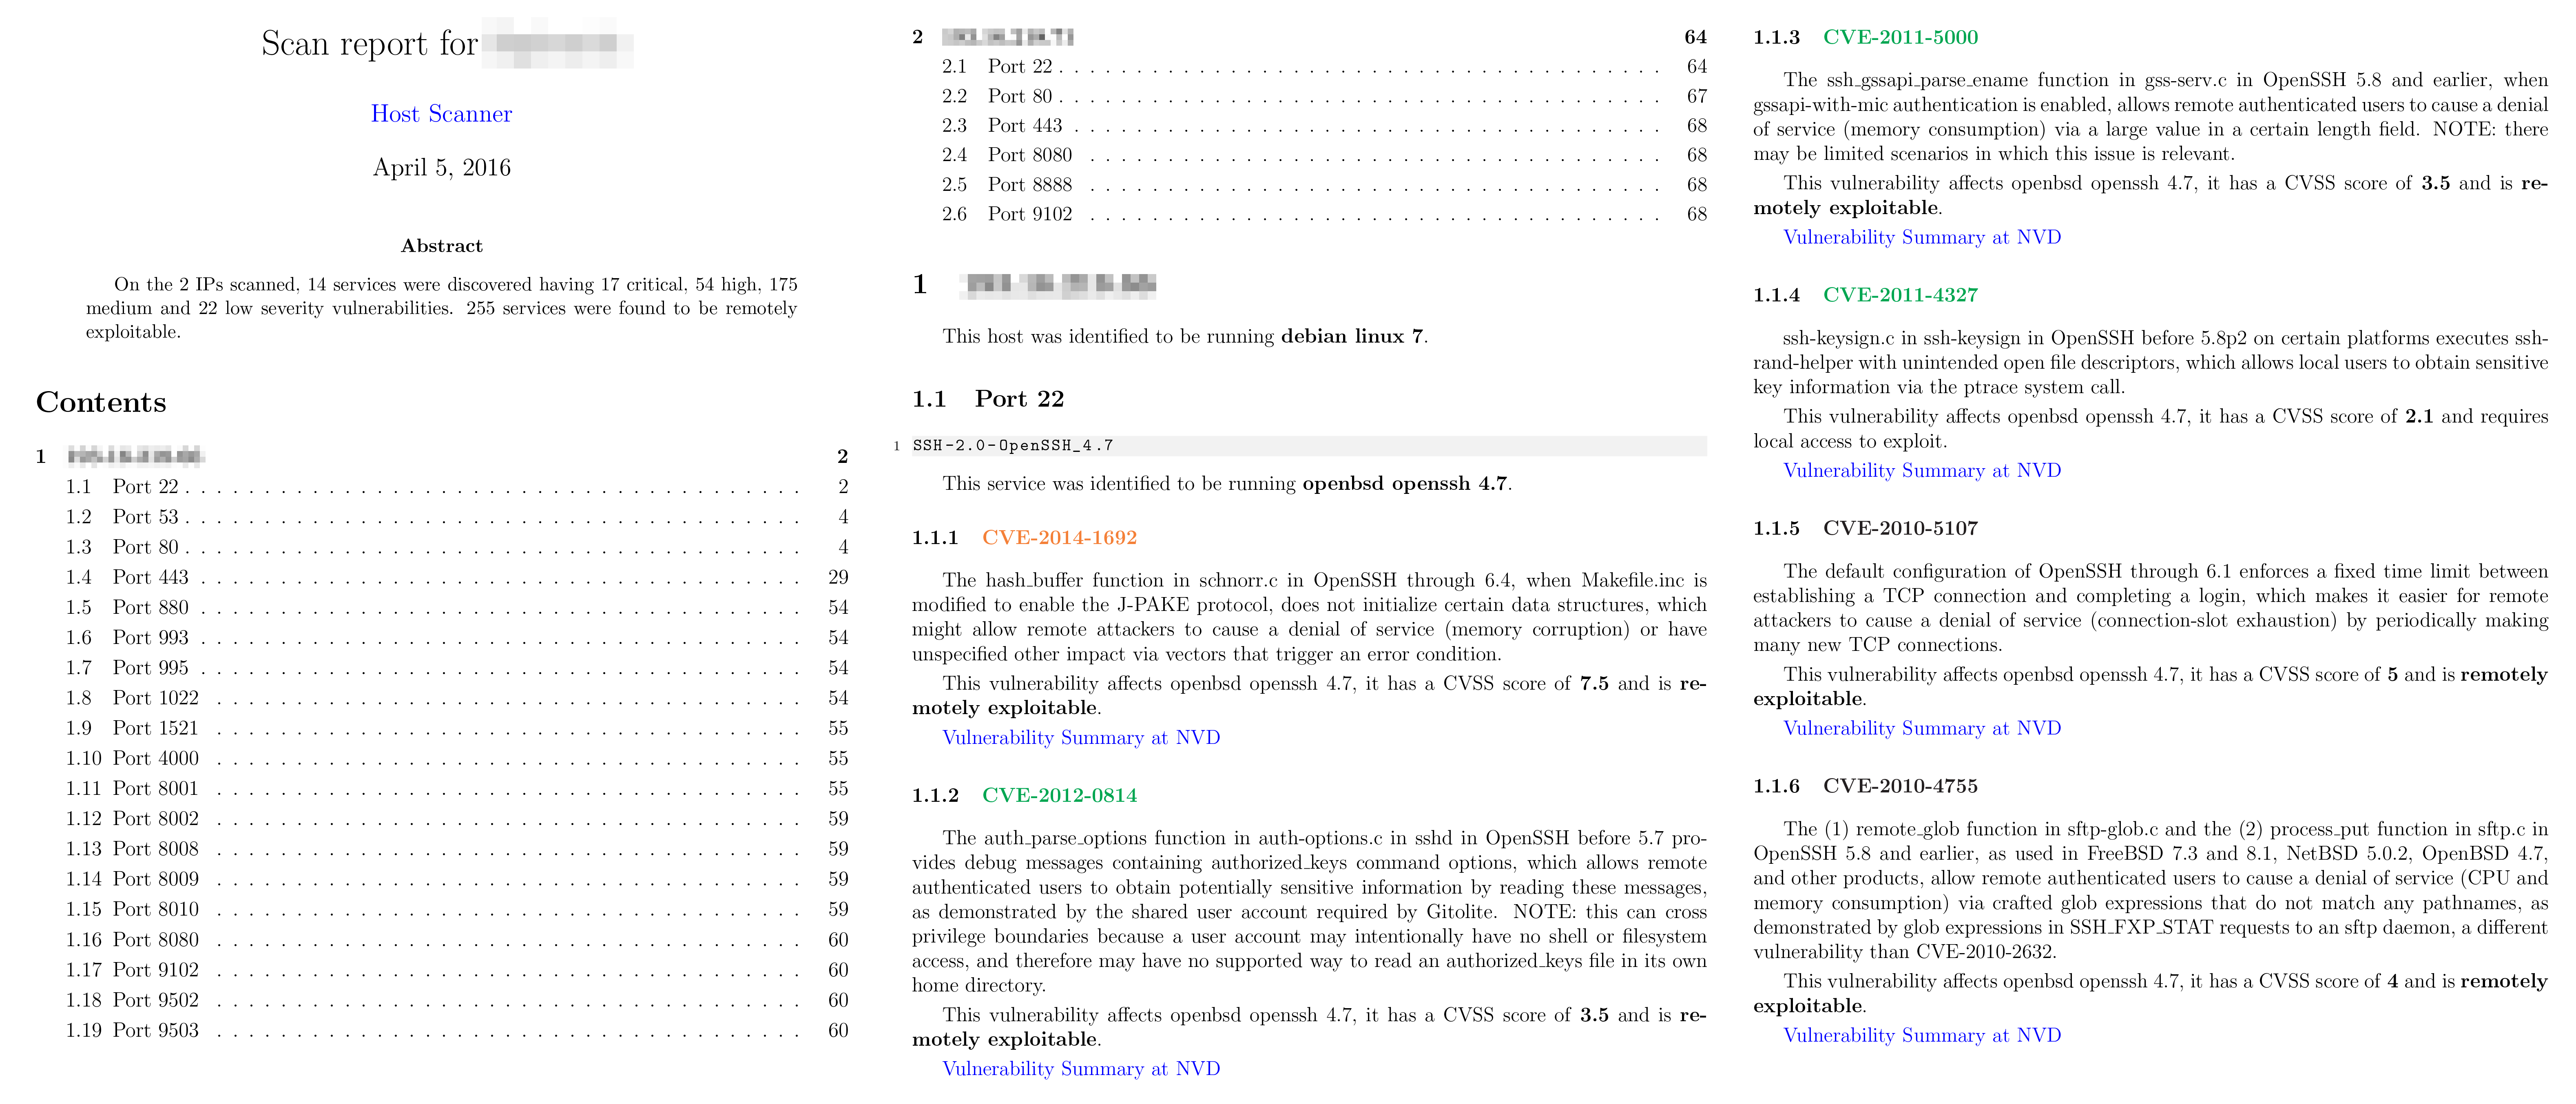
\includegraphics[scale=0.07]{reportcap.png}
		\caption{\LaTeX\ report generated after a scan session}
		\label{latexrep}
	\end{figure}
	
\subsection{Command Line Options} \label{cliopts}
\subsectionhu{Parancssori Opciók} \subsectionro{Opțiuni ale Interfeței CLI}

	\begin{minted}[linenos=false,bgcolor=]{mathematica}
usage:		HostScanner.exe [args] targets
arguments:

-t [ --target ] arg

  List of targets to scan:
    Each can be a hostname, IP address, IP range or CIDR.
    E.g. `192.168.1.1/24` is equivalent to `192.168.1.0-192.168.1.255`.

-p [ --port ] arg

  TCP ports to scan:
    Can be a single port (80), a list (22,80) or a range (1-1024).
    Range can be unbounded from either sides, simultaneously.
    E.g. `1024-` will scan ports 1024-65535. `-` will scan all ports.
    Specifying `top` or `t` will scan the top 100 most popular ports.

-u [ --udp-port ] arg

  UDP ports to scan:
    Supports the same values as --port, with the difference that
    specifying `top` will scan all of the ports with known payloads.

-s [ --scanner ] arg

  Scanner instance to use:
    internal - Uses the built-in scanner. (active)
    nmap     - Uses 3rd-party application Nmap. (active)
    shodan   - Uses data from Shodan. (passive; requires API key)
    censys   - Uses data from Censys. (passive; requires API key)
    looquer  - Uses data from Mr Looquer. (passive; requires API key)
    shosys   - Uses data from Shodan, Censys and Mr Looquer. (passive)

--shodan-key arg

  Specifies an API key for Shodan.

--shodan-uri arg

  Overrides the API endpoint used for Shodan. You may specify an URI
    starting with file:// pointing to a directory containing previously
    downloaded JSON responses.
      Default: https://api.shodan.io/shodan

--censys-key arg

  Specifies an API key for Censys in the `uid:secret` format.

--censys-uri arg

  Overrides the API endpoint used for Censys. You may specify an URI
    starting with file:// pointing to a directory containing previously
    downloaded JSON responses.
      Default: https://censys.io/api/v1

--looquer-key arg

  Specifies an API key for Mr Looquer.

--looquer-uri arg

  Overrides the API endpoint used for Mr Looquer. You may specify an URI
    starting with file:// pointing to a directory containing previously
    downloaded JSON responses.
      Default: https://mrlooquer.com/api/v1

-f [ --input-file ] arg

  Process an input file with the selected scanner.
    E.g. the nmap scanner can parse XML reports.

-d [ --delay ] arg

  Delay between packets sent to the same host. Default is 3 for 100ms.
    Possible values are 0..6, which have the same effect as nmap's -T:
      0 - 5m, 1 - 15s, 2 - 400ms, 3 - 100ms, 4 - 10ms, 5 - 5ms,
      6 - no delay

-r [ --resolve ]

  Resolves vulnerable CPE names to their actual package names depending
    on the automatically detected operating system of the host.

-o [ --output-latex ] arg

  Exports the scan results into a LaTeX file, with all the available
    information gathered during the scan.

-x [ --passive ]

  Globally disables active reconnaissance. Functionality using active
    scanning will break, but ensures no accidental active scans will be
    initiated, which might get construed as hostile.

-l [ --logging ] arg

  Logging level to use:
    i, int - All messages.
    d, dbg - All debug messages and up.
    v, vrb - Enable verbosity, but don't overdo it.
    m, msg - Print only regular messages. (default)
    e, err - Print only error messages to stderr.

-q [ --no-logo ]

  Suppresses the ASCII logo.

-v [ --version ]

  Display version information.

-h [ --help ]

  Displays this message.
	\end{minted}
	\vspace{-0.3in}
	\begin{listing}[H]
		\caption{Command line interface options}
		\label{clihelp}
	\end{listing}

\section{Results}
\sectionhu{Eredmények} \sectionro{Rezultate}

	The application was tested against three higher education institutions with both active and passive scanning methods. After these tests have concluded, another one was conducted with only passive scanning against five randomly selected leading\footnote{Based on amount of assets held as per their individual performance reports for the year 2015.} banking institutions, which I would have expected to represent the ``gold standard'' in the test.

	\begin{table}[H]
		\centering
		\begin{tabular}{r|ccc|ccc|ccccc|}
			\cline{2-12}
			\multicolumn{1}{l|}{}                         & \multicolumn{3}{c|}{\textbf{Active Scan}} & \multicolumn{8}{c|}{\textbf{Passive Scan}}                                                             \\ \hline
			\multicolumn{1}{|r|}{\textbf{Institution}}      & \textbf{$u_1$}    & \textbf{$u_2$}    & \textbf{$u_3$}   & \textbf{$u_1$} & \textbf{$u_2$} & \textbf{$u_3$} & \textbf{$b_1$} & \textbf{$b_2$} & \textbf{$b_3$} & \textbf{$b_4$} & \textbf{$b_5$} \\ \hline
			\multicolumn{1}{|r|}{\textbf{Services}} & 165            & 178            & 455           & 201         & 269         & 623         & 41          & 19          & 69          & 31          & 11          \\
			\multicolumn{1}{|r|}{\textbf{Identifiable}} & 143            & 145            & 402           & 112         & 148         & 352         & 24          & 8           & 58          & 9           & 9           \\
			\multicolumn{1}{|r|}{\textbf{Identified}}   & 140            & 137            & 394           & 109         & 139         & 348         & 24          & 8           & 58          & 9           & 9           \\ \hline
		\end{tabular}
		\caption{Identifiable services and the number of CPE names identified by the application}
		\label{cpeids}
	\end{table}
	
	Table \ref{cpeids} presents the number of services discovered at the tested institutions for each scanning attempt. The ``Services'' row represents an \textit{open port}. The ``Identifiable'' row represents the services which have replied with a service banner, and at the same time that service banner contains enough information for the service to be properly identified under normal conditions, such as its software name and version number. This number was determined through manual verification of the service banners for this test. The ``Identified'' row represents the number of services correctly identified by the software.
	
	Out of the \textbf{1,410} identifiable service banners, \textbf{1,374} services were correctly identified by the application, resulting in a success rate of \textbf{97.45\%}.
	
	\begin{table}[H]
		\centering
		\begin{tabular}{r|ccc|ccc|ccccc|}
			\cline{2-12}
			\multicolumn{1}{l|}{}                         & \multicolumn{3}{c|}{\textbf{Active Scan}} & \multicolumn{8}{c|}{\textbf{Passive Scan}}                                                             \\ \hline
			\multicolumn{1}{|r|}{\textbf{Institution}}      & \textbf{$u_1$}    & \textbf{$u_2$}    & \textbf{$u_3$}   & \textbf{$u_1$} & \textbf{$u_2$} & \textbf{$u_3$} & \textbf{$b_1$} & \textbf{$b_2$} & \textbf{$b_3$} & \textbf{$b_4$} & \textbf{$b_5$} \\
			\multicolumn{1}{|r|}{\textbf{Services}} & 165            & 178            & 455           & 201         & 269         & 623         & 41          & 19          & 69          & 31          & 11          \\ \hline
			\multicolumn{1}{|r|}{\textbf{Critical}}       & 183            & 121            & 160           & 161         & 131         & 230         & 8           & 0           & 30          & 6           & 6           \\
			\multicolumn{1}{|r|}{\textbf{High}}          & 675            & 414            & 645           & 583         & 446         & 826         & 7           & 0           & 67          & 21          & 5           \\
			\multicolumn{1}{|r|}{\textbf{Medium}}        & 2545           & 1441           & 2775          & 2308        & 1589        & 3247        & 19          & 0           & 299         & 133         & 9           \\
			\multicolumn{1}{|r|}{\textbf{Low}}       & 231            & 151            & 275           & 195         & 170         & 335         & 7           & 0           & 26          & 13          & 4           \\
			\multicolumn{1}{|r|}{\textbf{AV:N}}           & 3296           & 1970           & 3493          & 2961        & 2173        & 4248        & 40          & 0           & 393         & 153         & 22          \\ \hline
		\end{tabular}
		\caption{Discovered vulnerabilities of the services identified by the application}
		\label{cpevulns}
	\end{table}
	
	Table \ref{cpevulns} presents the number of vulnerabilities found on the services which have been discovered and successfully identified. The ``Critical,'' ``High,'' ``Medium'' and ``Low'' rows represent the number of vulnerabilities discovered for each severity level, while the ``AV:N'' row presents the number of vulnerabilities which can be remotely exploited over a network connection. (This information is available from the \textit{CVSS} scoring system presented in section \ref{cvss}, where the ``Access Vector'' field has the ``Network'' level associated to it.)
	
	The number of vulnerabilities discovered in the IP ranges of the banking institutions is unfortunately not surprising, as with a related project\footnote{\url{https://github.com/RoliSoft/Bank-Security-Audit}} of mine, I measured the response time of various banks to patching newly discovered critical vulnerabilities (such as Heartbleed, Shellshock, POODLE) and I've come to the conclusion, that some banks require up to 3 months in order to apply a security update for a critical vulnerability.
	
	\begin{table}[H]
		\centering
		\begin{tabular}{|r|l|}
			\hline
			\multicolumn{1}{|c|}{\textbf{Software}} & \multicolumn{1}{c|}{\textbf{CVE\#}} \\ \hline
			\textit{Host Scanner\footnotemark{}}                   & 166                                 \\
			OpenVAS                                 & 107                                 \\
			Nessus                                  & 68                                  \\
			Nexpose                                 & 311                                 \\ \hline
		\end{tabular}
		\caption{Comparison of identified vulnerabilities by competing software}
		\label{foundvulns}
	\end{table}
	\footnotetext{Name of the application developed within the scope of this thesis.}
	
	As a second test, the application was compared to the commercial tools discussed in section \ref{comtools}. Since these applications make a lot of noise (as in, network traffic) plus might take too much time to complete besides potentially overloading the services, not to mention potential licensing issues (most of them only allow home use for the free/community editions, defined as scanning one private $/24$ IP range), rescanning the institutions in table \ref{cpevulns} would not be feasible.
	
	The scan targets were instead comprised of virtual machines on a virtual network, compiled of vulnerable machines which were made for the express purpose of CTF (``Capture the Flag'') style wargames, such as \textit{Metasploitable} and \textit{VulnOS}. These VM images were gathered from VulnHub\footnote{\url{https://www.vulnhub.com/}}, as suggested in article \cite{penintro15} and paper \cite{secgen15}, a website whose aim is to provide downloadable VM images which simulate a real-world vulnerable infrastructure in order to allow interested parties to practice and gain hands-on penetration testing experience without breaking the law.
	
	The weak results of ``OpenVAS'' and ``Nessus'' can be explain with the fact that their extension-based architecture failed to identify various obscure services on these hosts, as they did not have an extension written for them, and failing to identify some crucial services resulted in a decreased CVE count.
	
	On the other side of the spectrum, ``Nexpose'' exploited one of the discovered vulnerabilities, and using the acquired shell access, enumerated the list of installed packages using the operating system's package manager, gaining a clear advantage, as the other three testing applications only analyzed the vulnerability status of public-facing network-accessible servers, without having access to the full list of installed software on the host.
	
	It should be noted, that exploitation of the discovered vulnerabilities is out of the scope of this application, as it may not be desirable in live production environments, and straight-up illegal for security researchers without a prior agreement. In the application, vulnerability validation is instead performed without penetration, by gathering environmental information, identifying the operating system, and then using the operating system distribution's package manager to check whether the discovered package is affected by the vulnerability, as described in section \ref{vulnvalid}.

\newpage
\section{Bibliography}
\sectionhu{Bibliográfia} \sectionro{Bibliografie}

	\begingroup
	\renewcommand{\section}[2]{}
	\renewcommand{\markboth}[2]{}
		\bibliography{thesis}
		\bibliographystyle{thesis}
	\endgroup

	\vfill

	\begin{wrapfigure}{r}{0.22\textwidth}
		\vspace{-22pt}
		\begin{flushright}
			{\Huge \ccbysa}
		\end{flushright}
	\end{wrapfigure}

	\noindent This thesis is licensed under the \textit{Creative Commons Attribution-ShareAlike 4.0 International License}. To view a copy of this license, visit \url{http://creativecommons.org/licenses/by-sa/4.0/}.

\end{document}
